\documentclass[12pt,english,nohyper]{tufte-handout}\usepackage[]{graphicx}\usepackage[]{color}
%% maxwidth is the original width if it is less than linewidth
%% otherwise use linewidth (to make sure the graphics do not exceed the margin)
\makeatletter
\def\maxwidth{ %
  \ifdim\Gin@nat@width>\linewidth
    \linewidth
  \else
    \Gin@nat@width
  \fi
}
\makeatother

\definecolor{fgcolor}{rgb}{0.345, 0.345, 0.345}
\newcommand{\hlnum}[1]{\textcolor[rgb]{0.686,0.059,0.569}{#1}}%
\newcommand{\hlstr}[1]{\textcolor[rgb]{0.192,0.494,0.8}{#1}}%
\newcommand{\hlcom}[1]{\textcolor[rgb]{0.678,0.584,0.686}{\textit{#1}}}%
\newcommand{\hlopt}[1]{\textcolor[rgb]{0,0,0}{#1}}%
\newcommand{\hlstd}[1]{\textcolor[rgb]{0.345,0.345,0.345}{#1}}%
\newcommand{\hlkwa}[1]{\textcolor[rgb]{0.161,0.373,0.58}{\textbf{#1}}}%
\newcommand{\hlkwb}[1]{\textcolor[rgb]{0.69,0.353,0.396}{#1}}%
\newcommand{\hlkwc}[1]{\textcolor[rgb]{0.333,0.667,0.333}{#1}}%
\newcommand{\hlkwd}[1]{\textcolor[rgb]{0.737,0.353,0.396}{\textbf{#1}}}%

\usepackage{framed}
\makeatletter
\newenvironment{kframe}{%
 \def\at@end@of@kframe{}%
 \ifinner\ifhmode%
  \def\at@end@of@kframe{\end{minipage}}%
  \begin{minipage}{\columnwidth}%
 \fi\fi%
 \def\FrameCommand##1{\hskip\@totalleftmargin \hskip-\fboxsep
 \colorbox{shadecolor}{##1}\hskip-\fboxsep
     % There is no \\@totalrightmargin, so:
     \hskip-\linewidth \hskip-\@totalleftmargin \hskip\columnwidth}%
 \MakeFramed {\advance\hsize-\width
   \@totalleftmargin\z@ \linewidth\hsize
   \@setminipage}}%
 {\par\unskip\endMakeFramed%
 \at@end@of@kframe}
\makeatother

\definecolor{shadecolor}{rgb}{.97, .97, .97}
\definecolor{messagecolor}{rgb}{0, 0, 0}
\definecolor{warningcolor}{rgb}{1, 0, 1}
\definecolor{errorcolor}{rgb}{1, 0, 0}
\newenvironment{knitrout}{}{} % an empty environment to be redefined in TeX

\usepackage{alltt}
\usepackage[T1]{fontenc}
\usepackage[utf8]{inputenc}
\usepackage{longtable}
\usepackage{wrapfig}
\usepackage{hyperref}
\usepackage{graphicx}
\usepackage[space]{grffile}
\usepackage{enumitem}

%\usepackage[letterpaper]{geometry}
%\geometry{verbose,tmargin=4cm,bmargin=4.5cm,lmargin=3.2cm,rmargin=3.5cm}
%\usepackage{setspace}
%\usepackage{fullpage}
%\usepackage{tikz}
%\onehalfspacing

\makeatletter
%%%%%%%%%%%%%%%%%%%%%%%%%%%%%% Textclass specific LaTeX commands.
\newcommand{\Rcode}[1]{{\texttt{#1}}}
\newcommand{\Robject}[1]{{\texttt{#1}}}
\newcommand{\Rcommand}[1]{{\texttt{#1}}}
\newcommand{\Rfunction}[1]{{\texttt{#1}}}
\newcommand{\Rfunarg}[1]{{\textit{#1}}}
\newcommand{\Rpackage}[1]{{\textit{#1}}}
\newcommand{\Rmethod}[1]{{\textit{#1}}}
\newcommand{\Rclass}[1]{{\textit{#1}}}
\makeatother
\IfFileExists{upquote.sty}{\usepackage{upquote}}{}
\begin{document}

% Font of caption must be specified, otherwise gray
\setcaptionfont{
  \normalfont\footnotesize
  \color{black}
}





\centerline{\Large\bf Introductory Statistics Homework Analysis}


\section{Overview}
The file name with student responses and scores is Topic03.AB.csv. 50 students submitted the homework assignment.

Full credit for this homework assignment is 35. Each student was given 31 questions and this homework assignment contains a total of 86 questions.  

The mean score of the 50 students who submited the homework assignment is 8.33. The lowest and highest scores are 0 and 31, respectively.

The histogram and summary statistics for the scores are given by Figure \ref{mar:histScore} and Table \ref{tab:summary}.

\begin{knitrout}
\definecolor{shadecolor}{rgb}{0.969, 0.969, 0.969}\color{fgcolor}\begin{marginfigure}
\includegraphics[width=0.98\linewidth]{/private/var/folders/vn/lhzbs8ds6xbg965nnfcj6ftm0000gn/T/Rtmp9RBshrhistScore-1} \caption[Histogram of scores]{Histogram of scores.}\label{mar:histScore}
\end{marginfigure}


\end{knitrout}

% latex table generated in R 3.2.2 by xtable 1.8-0 package
% Fri Nov 27 10:29:24 2015
\begin{longtable}{rrlrrrrr}
  \hline
Mean & Std.dev &   & Min & Q1 & Median & Q3 & Max \\ 
  \hline
8.33 & 6.56 &  & 0.00 & 5.00 & 6.00 & 8.00 & 31.00 \\ 
   \hline
\hline
\caption{Summary statistics of the scores} 
\label{tab:summary}
\end{longtable}


\clearpage
\newpage{}
\section{Topic Learning Outcomes}

\bigskip{}

\begin{fullwidth}
\begin{enumerate}[label=\Alph*.,itemsep=-\parsep,leftmargin=*]
  \item
Identify a quantitative variable.
\item Identify appropriate displays of a quantitative variable.
\item Identify and interpret components of a histogram.
\item Describe the shape of the distribution of a quantitative variable using a histogram or stem-and-leaf display.
\item Identify important characteristics of the distribution of a quantitative variable using a histogram or stem-and-leaf display.
\item Identify potential outliers in a distribution using a histogram or stem-and-leaf display.
\item Report the 5-number summary for a quantitative variable.
\item Calculate the 5-number summary for a quantitative variable.
\item Describe the important characteristics of the 5-number summary.
\item Report the values of the mean and standard deviation for a quantitative variable.
\item Calculate the mean and standard deviation for a quantitative variable.
\item Describe the important characteristics of the mean and standard deviation.
\item Compare and contrast the median and the mean as numerical summaries of the center of the distribution of a quantitative variable.
\item Compare and contrast the range, interquartile range and the standard deviation as numerical summaries of the variability of the distribution of a quantitative variable.
\item Identify the most appropriate measures of center and variability to use for a particular quantitative variable.

\end{enumerate}
\end{fullwidth}

\newpage{}

Table \ref{tab:LearningObj_summary} and Figure \ref{mar:LearningObjSummary} show the summary of percentage scores by learning outcome.
Among all learning outcomes, Outcome
M
has the highest correct percentage, while Outcome
K
has the lowest.



\begin{knitrout}
\definecolor{shadecolor}{rgb}{0.969, 0.969, 0.969}\color{fgcolor}\begin{marginfigure}
\includegraphics[width=0.98\linewidth]{/private/var/folders/vn/lhzbs8ds6xbg965nnfcj6ftm0000gn/T/Rtmp9RBshrLearningObjSummary-1} \caption[Side-by-side boxplots of the correct percentages by learning outcome]{Side-by-side boxplots of the correct percentages by learning outcome.}\label{mar:LearningObjSummary}
\end{marginfigure}


\end{knitrout}

% latex table generated in R 3.2.2 by xtable 1.8-0 package
% Fri Nov 27 10:29:25 2015
\begin{longtable}{rrrllrrr}
  \hline
 & Mean & Std.dev &   &   & Min & Median & Max \\ 
  \hline
M & 36.50 & 30.39 &  &  & 0.00 & 25.00 & 100.00 \\ 
  O & 35.00 & 39.45 &  &  & 0.00 & 25.00 & 100.00 \\ 
  F & 34.00 & 47.85 &  &  & 0.00 & 0.00 & 100.00 \\ 
  D & 30.00 & 37.80 &  &  & 0.00 & 0.00 & 100.00 \\ 
  C & 28.80 & 26.85 &  &  & 0.00 & 20.00 & 100.00 \\ 
  L & 28.00 & 27.96 &  &  & 0.00 & 25.00 & 100.00 \\ 
  H & 26.00 & 44.31 &  &  & 0.00 & 0.00 & 100.00 \\ 
  N & 22.00 & 30.57 &  &  & 0.00 & 0.00 & 100.00 \\ 
  I & 20.50 & 36.31 &  &  & 0.00 & 0.00 & 100.00 \\ 
  A & 20.00 & 40.41 &  &  & 0.00 & 0.00 & 100.00 \\ 
  B & 20.00 & 40.41 &  &  & 0.00 & 0.00 & 100.00 \\ 
  E & 18.67 & 26.22 &  &  & 0.00 & 0.00 & 100.00 \\ 
  J & 6.50 & 15.82 &  &  & 0.00 & 0.00 & 50.00 \\ 
  G & 6.00 & 23.99 &  &  & 0.00 & 0.00 & 100.00 \\ 
  K & 0.00 & 0.00 &  &  & 0.00 & 0.00 & 0.00 \\ 
   \hline
\hline
\caption{Summary statistics of the student percentage correct scores on the topic learning outcomes. The table is sorted from the highest mean to the lowest.} 
\label{tab:LearningObj_summary}
\end{longtable}






To analyze the students' performance on different learning outcomes, we consider the generalized mixed effects model:
\[
g(E[Y_{ij}|u_{j}])= \tau_{i}+u_{j}
\]
where $i=1,...,$15 learning outcomes;
$j=1,...,$50 students. $Y_{ij}$ is the score (scaled in $[0,1]$) of
the $j$th student in the $i$th learning outcome. $\tau_i$ is the fixed effect,
which represents the actual level of the learning outcome $i$.
$u_j$ is the random effect from the students with
$u_{j} \sim N(0,\sigma_{u}^{2})$.

Since $Y_{ij} \in [0,1]$, and most of $y_{ij}$ take the value 1
(see Figure \ref{mar:crtpctHist}), it is not easy to find an appropriate model.
Beta distribution is possible if 0 and 1 are not in the range of $Y_{ij}$.
Binomial distribution is another possibility if we do not scale the scores.
Hence we assume that $Y$ is binomial with the logit link function,
then the results are in Table \ref{tab:lme_fixed} and Figure \ref{mar:lmeCoef}.

\begin{knitrout}
\definecolor{shadecolor}{rgb}{0.969, 0.969, 0.969}\color{fgcolor}\begin{marginfigure}
\includegraphics[width=0.99\linewidth]{/private/var/folders/vn/lhzbs8ds6xbg965nnfcj6ftm0000gn/T/Rtmp9RBshrcrtpctHist-1} \caption[Histogram of the scaled scores by learning outcome]{Histogram of the scaled scores by learning outcome.}\label{mar:crtpctHist}
\end{marginfigure}


\end{knitrout}

% latex table generated in R 3.2.2 by xtable 1.8-0 package
% Fri Nov 27 10:29:27 2015
\begin{longtable}{rrlrr}
  \hline
 & est. &    & lower & upper \\ 
  \hline
(Intercept) & -0.55 &  & -1.05 & -0.06 \\ 
  ObjectiveO & -0.07 &  & -0.66 & 0.51 \\ 
  ObjectiveF & -0.12 &  & -0.71 & 0.46 \\ 
  ObjectiveD & -0.33 &  & -0.93 & 0.26 \\ 
  ObjectiveC & -0.40 &  & -1.00 & 0.20 \\ 
  ObjectiveL & -0.44 &  & -1.05 & 0.16 \\ 
  ObjectiveH & -0.56 &  & -1.17 & 0.05 \\ 
  ObjectiveN & -0.81 &  & -1.44 & -0.18 \\ 
  ObjectiveI & -0.91 &  & -1.55 & -0.27 \\ 
  ObjectiveA & -0.95 &  & -1.59 & -0.30 \\ 
  ObjectiveB & -0.95 &  & -1.59 & -0.30 \\ 
  ObjectiveE & -1.05 &  & -1.70 & -0.39 \\ 
  ObjectiveJ & -2.37 &  & -3.25 & -1.49 \\ 
  ObjectiveG & -2.46 &  & -3.36 & -1.56 \\ 
  ObjectiveK & -4.64 &  & -6.58 & -2.70 \\ 
   \hline
\hline
\caption{95\% confidence intervals of the fixed effects} 
\label{tab:lme_fixed}
\end{longtable}


It shows that M is the best understood learning outcome.
Outcomes K,G,J,E,B,A,I,N,M are
significantly worse than M.



\begin{knitrout}
\definecolor{shadecolor}{rgb}{0.969, 0.969, 0.969}\color{fgcolor}\begin{marginfigure}
\includegraphics[width=0.99\linewidth]{/private/var/folders/vn/lhzbs8ds6xbg965nnfcj6ftm0000gn/T/Rtmp9RBshrlmeCoef-1} \caption[95\% confidence intervals of the fixed effects coefficients]{95\% confidence intervals of the fixed effects coefficients}\label{mar:lmeCoef}
\end{marginfigure}


\end{knitrout}

Nevertheless, the assumption is probably incorrect, as we could check the residuals in
Figure \ref{fig:lmeQQNorm}.

\begin{knitrout}
\definecolor{shadecolor}{rgb}{0.969, 0.969, 0.969}\color{fgcolor}\begin{figure}

{\centering \includegraphics[width=0.98\linewidth]{/private/var/folders/vn/lhzbs8ds6xbg965nnfcj6ftm0000gn/T/Rtmp9RBshrlmeQQNorm-1} 

}

\caption[QQ-plot of the residuals by the generalized mixed effects model]{QQ-plot of the residuals by the generalized mixed effects model}\label{fig:lmeQQNorm}
\end{figure}


\end{knitrout}

\clearpage
\newpage{}
\subsection{Question Sets}

Table \ref{tab:QuestionSet_summary} and Figure \ref{mar:questionSetBoxplot} shows the summary statistics of the percentage correct score by question for each question set. Percentage correct scores for questions in the same question set should have small variability.
%As is shown, Question Set colnames(sumry2$SetCorrectPct)[which.max(sumry2$SetCorrectPct[1,])] has the highest mean correct percentage and question set colnames(sumry2$SetCorrectPct)[which.min(sumry2$SetCorrectPct[1,])] has the lowest mean.


% latex table generated in R 3.2.2 by xtable 1.8-0 package
% Fri Nov 27 10:29:28 2015
\begin{longtable}{cc|ccc|ccc}
  \hline
Qset & LO & \# & Mean & Std.dev & Min & Median & Max \\ 
  \hline
AA & O &   2 & 41.23 & 21.63 & 25.93 & 41.23 & 56.52 \\ 
  L & H &   4 & 28.87 & 17.83 & 7.14 & 29.16 & 50.00 \\ 
  B & B &   2 & 21.27 & 14.93 & 10.71 & 21.27 & 31.82 \\ 
  J & F &   4 & 34.04 & 14.71 & 15.38 & 35.38 & 50.00 \\ 
  U & M &   2 & 42.45 & 14.40 & 32.26 & 42.45 & 52.63 \\ 
  C & C &   3 & 37.87 & 13.09 & 29.41 & 31.25 & 52.94 \\ 
  AB & O &   3 & 30.06 & 11.99 & 21.43 & 25.00 & 43.75 \\ 
  V & M &   3 & 42.26 & 11.21 & 29.41 & 47.37 & 50.00 \\ 
  G & C &   4 & 19.26 & 10.54 & 8.33 & 17.69 & 33.33 \\ 
  T & L &   3 & 30.54 & 8.94 & 22.22 & 29.41 & 40.00 \\ 
  M & I &   3 & 20.61 & 8.53 & 11.11 & 23.08 & 27.63 \\ 
  S & L &   3 & 18.32 & 7.21 & 10.00 & 22.22 & 22.73 \\ 
  H & D &   4 & 30.13 & 6.82 & 23.08 & 29.15 & 39.13 \\ 
  W & M &   3 & 42.67 & 6.71 & 36.84 & 41.18 & 50.00 \\ 
  D & C &   3 & 23.30 & 6.39 & 16.67 & 23.81 & 29.41 \\ 
  A & A &   4 & 18.73 & 5.73 & 14.29 & 17.14 & 26.32 \\ 
  K & G &   4 & 6.16 & 4.53 & 0.00 & 7.32 & 10.00 \\ 
  F & C &   4 & 27.31 & 4.42 & 22.22 & 27.88 & 31.25 \\ 
  N & J &   4 & 6.55 & 4.27 & 1.79 & 6.44 & 11.54 \\ 
  I & E &   6 & 18.73 & 4.09 & 13.64 & 18.23 & 23.53 \\ 
  Z & N &   3 & 26.02 & 3.35 & 22.22 & 27.27 & 28.57 \\ 
  E & C &   3 & 34.12 & 1.37 & 33.33 & 33.33 & 35.71 \\ 
  O & K &   4 & 0.00 & 0.00 & 0.00 & 0.00 & 0.00 \\ 
  P & K &   4 & 0.00 & 0.00 & 0.00 & 0.00 & 0.00 \\ 
  Q & L &   1 & 32.00 & 0.00 & 32.00 & 32.00 & 32.00 \\ 
  R & L &   1 & 30.00 & 0.00 & 30.00 & 30.00 & 30.00 \\ 
  X & M &   1 & 22.00 & 0.00 & 22.00 & 22.00 & 22.00 \\ 
  Y & N &   1 & 18.00 & 0.00 & 18.00 & 18.00 & 18.00 \\ 
   \hline
\hline
\caption{Summary statistics of the percentage correct score by question for each question sets. The table is sorted from the largest standard deviation to the smallest.} 
\label{tab:QuestionSet_summary}
\end{longtable}


\begin{knitrout}
\definecolor{shadecolor}{rgb}{0.969, 0.969, 0.969}\color{fgcolor}\begin{marginfigure}

{\centering \includegraphics[width=0.99\linewidth]{/private/var/folders/vn/lhzbs8ds6xbg965nnfcj6ftm0000gn/T/Rtmp9RBshrquestionSetBoxplot-1} 

}

\caption[Side-by-side boxplots of the question correct percentage score for each question set]{Side-by-side boxplots of the question correct percentage score for each question set}\label{fig:questionSetBoxplot}
\end{marginfigure}


\end{knitrout}

\clearpage
\newpage{}
\subsection{Questions}

Table \ref{tab:summary_question} compares the performance on each question.



% latex table generated in R 3.2.2 by xtable 1.8-0 package
% Fri Nov 27 10:29:30 2015
\begin{longtable}{cccl|cccc|ccccc|l}
  \hline
ID & LO & Qset & Name & Type & FullPt & QinSet & N & CrtPct & Count & NA's & Mean & Std & Flag \\ 
  \hline
\hyperlink{T03.A.A.04.1.1.MU.1.2}{1} & A & A & 1 & MU &   1 &   1 &   4 & 20.00 &  10 &  40 & 0.20 & 0.42 &  \\ 
  \hyperlink{T03.A.A.04.1.1.MU.2.2}{2} & A & A & 2 & MU &   1 &   1 &   4 & 26.32 &  19 &  31 & 0.26 & 0.45 &  \\ 
  \hyperlink{T03.A.A.04.1.1.MU.3.2}{3} & A & A & 3 & MU &   1 &   1 &   4 & 14.29 &   7 &  43 & 0.14 & 0.38 &  \\ 
  \hyperlink{T03.A.A.04.1.1.MU.4.2}{4} & A & A & 4 & MU &   1 &   1 &   4 & 14.29 &  14 &  36 & 0.14 & 0.36 &  \\ 
  \hyperlink{T03.B.B.02.1.1.MC.salaries1.2}{5} & B & B & salaries1 & MC &   1 &   1 &   2 & 31.82 &  22 &  28 & 0.32 & 0.48 & * \\ 
  \hyperlink{T03.B.B.02.1.1.MC.salaries2.2}{6} & B & B & salaries2 & MC &   1 &   1 &   2 & 10.71 &  28 &  22 & 0.11 & 0.31 & * \\ 
   &  &  &  &  &  &  &  &  &  &  &  &  &  \\ 
  \hyperlink{T03.C.C.03.1.1.MC.horizontal.2}{7} & C & C & horizontal & MC &   1 &   1 &   3 & 29.41 &  17 &  33 & 0.29 & 0.47 & * \\ 
  \hyperlink{T03.C.C.03.1.1.MC.horizontal2.2}{8} & C & C & horizontal2 & MC &   1 &   1 &   3 & 31.25 &  16 &  34 & 0.31 & 0.48 & * \\ 
  \hyperlink{T03.C.C.03.1.1.MC.horizontal3.2}{9} & C & C & horizontal3 & MC &   1 &   1 &   3 & 52.94 &  17 &  33 & 0.53 & 0.51 & * \\ 
   &  &  &  &  &  &  &  &  &  &  &  &  &  \\ 
  \hyperlink{T03.C.D.03.1.1.MC.vertical.2}{10} & C & D & vertical & MC &   1 &   1 &   3 & 23.81 &  21 &  29 & 0.24 & 0.44 &  \\ 
  \hyperlink{T03.C.D.03.1.1.MC.vertical2.2}{11} & C & D & vertical2 & MC &   1 &   1 &   3 & 29.41 &  17 &  33 & 0.29 & 0.47 &  \\ 
  \hyperlink{T03.C.D.03.1.1.MC.vertical3.2}{12} & C & D & vertical3 & MC &   1 &   1 &   3 & 16.67 &  12 &  38 & 0.17 & 0.39 &  \\ 
   &  &  &  &  &  &  &  &  &  &  &  &  &  \\ 
  \hyperlink{T03.C.E.03.1.1.MC.tips.2}{13} & C & E & tips & MC &   1 &   1 &   3 & 35.71 &  14 &  36 & 0.36 & 0.50 &  \\ 
  \hyperlink{T03.C.E.03.1.1.MC.tips2.2}{14} & C & E & tips2 & MC &   1 &   1 &   3 & 33.33 &  15 &  35 & 0.33 & 0.49 &  \\ 
  \hyperlink{T03.C.E.03.1.1.MC.tips3.2}{15} & C & E & tips3 & MC &   1 &   1 &   3 & 33.33 &  21 &  29 & 0.33 & 0.48 &  \\ 
   &  &  &  &  &  &  &  &  &  &  &  &  &  \\ 
  \hyperlink{T03.C.F.04.1.1.MC.flights1.2}{16} & C & F & flights1 & MC &   1 &   1 &   4 & 31.25 &  16 &  34 & 0.31 & 0.48 &  \\ 
  \hyperlink{T03.C.F.04.1.1.MC.flights2.2}{17} & C & F & flights2 & MC &   1 &   1 &   4 & 30.77 &  13 &  37 & 0.31 & 0.48 &  \\ 
  \hyperlink{T03.C.F.04.1.1.MC.flights3.2}{18} & C & F & flights3 & MC &   1 &   1 &   4 & 22.22 &   9 &  41 & 0.22 & 0.44 &  \\ 
  \hyperlink{T03.C.F.04.1.1.MC.flights4.2}{19} & C & F & flights4 & MC &   1 &   1 &   4 & 25.00 &  12 &  38 & 0.25 & 0.45 &  \\ 
   &  &  &  &  &  &  &  &  &  &  &  &  &  \\ 
  \hyperlink{T03.C.G.04.1.1.MC.flights5.2}{20} & C & G & flights5 & MC &   1 &   1 &   4 & 15.38 &  13 &  37 & 0.15 & 0.38 & * \\ 
  \hyperlink{T03.C.G.04.1.1.MC.flights6.2}{21} & C & G & flights6 & MC &   1 &   1 &   4 & 20.00 &  10 &  40 & 0.20 & 0.42 &  \\ 
  \hyperlink{T03.C.G.04.1.1.MC.flights7.2}{22} & C & G & flights7 & MC &   1 &   1 &   4 & 8.33 &  12 &  38 & 0.08 & 0.29 & * \\ 
  \hyperlink{T03.C.G.04.1.1.MC.flights8.2}{23} & C & G & flights8 & MC &   1 &   1 &   4 & 33.33 &  15 &  35 & 0.33 & 0.49 & * \\ 
   &  &  &  &  &  &  &  &  &  &  &  &  &  \\ 
  \hyperlink{T03.D.H.04.2.1.MC.random1.2}{24} & D & H & random1 & MC &   1 &   2 &   4 & 31.03 &  29 &  21 & 0.31 & 0.47 &  \\ 
  \hyperlink{T03.D.H.04.2.1.MC.random2.2}{25} & D & H & random2 & MC &   1 &   2 &   4 & 39.13 &  23 &  27 & 0.39 & 0.50 & * \\ 
  \hyperlink{T03.D.H.04.2.1.MC.random3.2}{26} & D & H & random3 & MC &   1 &   2 &   4 & 23.08 &  26 &  24 & 0.23 & 0.43 & * \\ 
  \hyperlink{T03.D.H.04.2.1.MC.random4.2}{27} & D & H & random4 & MC &   1 &   2 &   4 & 27.27 &  22 &  28 & 0.27 & 0.46 &  \\ 
   &  &  &  &  &  &  &  &  &  &  &  &  &  \\ 
  \hyperlink{T03.E.I.06.3.1.MC.blowhole.2}{28} & E & I & blowhole & MC &   1 &   3 &   6 & 13.64 &  22 &  28 & 0.14 & 0.35 &  \\ 
  \hyperlink{T03.E.I.06.3.1.MC.FEV.2}{29} & E & I & FEV & MC &   1 &   3 &   6 & 19.23 &  26 &  24 & 0.19 & 0.40 &  \\ 
  \hyperlink{T03.E.I.06.3.1.MC.diamonds.2}{30} & E & I & diamonds & MC &   1 &   3 &   6 & 15.38 &  26 &  24 & 0.15 & 0.37 &  \\ 
  \hyperlink{T03.E.I.06.3.1.MC.amps.2}{31} & E & I & amps & MC &   1 &   3 &   6 & 23.33 &  30 &  20 & 0.23 & 0.43 &  \\ 
  \hyperlink{T03.E.I.06.3.1.MC.lowtemp.2}{32} & E & I & lowtemp & MC &   1 &   3 &   6 & 17.24 &  29 &  21 & 0.17 & 0.38 &  \\ 
  \hyperlink{T03.E.I.06.3.1.MC.musicCDs.2}{33} & E & I & musicCDs & MC &   1 &   3 &   6 & 23.53 &  17 &  33 & 0.24 & 0.44 &  \\ 
   &  &  &  &  &  &  &  &  &  &  &  &  &  \\ 
  \hyperlink{T03.F.J.04.1.1.MC.blowhole.2}{34} & F & J & blowhole & MC &   1 &   1 &   4 & 15.38 &  13 &  37 & 0.15 & 0.38 & * \\ 
  \hyperlink{T03.F.J.04.1.1.MC.FEV.2}{35} & F & J & FEV & MC &   1 &   1 &   4 & 30.77 &  13 &  37 & 0.31 & 0.48 & * \\ 
  \hyperlink{T03.F.J.04.1.1.MC.amps.2}{36} & F & J & amps & MC &   1 &   1 &   4 & 50.00 &  14 &  36 & 0.50 & 0.52 & * \\ 
  \hyperlink{T03.F.J.04.1.1.MC.random2.2}{37} & F & J & random2 & MC &   1 &   1 &   4 & 40.00 &  10 &  40 & 0.40 & 0.52 & * \\ 
   &  &  &  &  &  &  &  &  &  &  &  &  &  \\ 
  \hyperlink{T03.G.K.04.1.1.MU.1.2}{38} & G & K & 1 & MU &   1 &   1 &   4 & 5.56 &  18 &  32 & 0.06 & 0.24 &  \\ 
  \hyperlink{T03.G.K.04.1.1.MU.2.2}{39} & G & K & 2 & MU &   1 &   1 &   4 & 10.00 &  10 &  40 & 0.10 & 0.32 &  \\ 
  \hyperlink{T03.G.K.04.1.1.MU.3.2}{40} & G & K & 3 & MU &   1 &   1 &   4 & 9.09 &  11 &  39 & 0.09 & 0.30 &  \\ 
  \hyperlink{T03.G.K.04.1.1.MU.4.2}{41} & G & K & 4 & MU &   1 &   1 &   4 & 0.00 &  11 &  39 & 0.00 & 0.00 &  \\ 
   &  &  &  &  &  &  &  &  &  &  &  &  &  \\ 
  \hyperlink{T03.H.L.04.1.1.MC.birthwt.2}{42} & H & L & birthwt & MC &   1 &   1 &   4 & 7.14 &  14 &  36 & 0.07 & 0.27 & * \\ 
  \hyperlink{T03.H.L.04.1.1.MC.heartrate.2}{43} & H & L & heartrate & MC &   1 &   1 &   4 & 25.00 &  16 &  34 & 0.25 & 0.45 & * \\ 
  \hyperlink{T03.H.L.04.1.1.MC.babe.2}{44} & H & L & babe & MC &   1 &   1 &   4 & 50.00 &   8 &  42 & 0.50 & 0.53 & * \\ 
  \hyperlink{T03.H.L.04.1.1.MC.hightemps.2}{45} & H & L & hightemps & MC &   1 &   1 &   4 & 33.33 &  12 &  38 & 0.33 & 0.49 & * \\ 
   &  &  &  &  &  &  &  &  &  &  &  &  &  \\ 
  \hyperlink{T03.I.M.03.1.4.FB.five1.2}{46} & I & M & five1 & FB &   4 &   1 &   3 & 23.08 &  13 &  37 & 0.92 & 1.75 &  \\ 
  \hyperlink{T03.I.M.03.1.4.FB.five2.2}{47} & I & M & five2 & FB &   4 &   1 &   3 & 27.63 &  19 &  31 & 1.11 & 1.70 & * \\ 
  \hyperlink{T03.I.M.03.1.4.FB.five3.2}{48} & I & M & five3 & FB &   4 &   1 &   3 & 11.11 &  18 &  32 & 0.44 & 0.78 & * \\ 
   &  &  &  &  &  &  &  &  &  &  &  &  &  \\ 
  \hyperlink{T03.J.N.04.1.2.FB.amps.2}{49} & J & N & amps & FB &   2 &   1 &   4 & 4.55 &  11 &  39 & 0.09 & 0.30 &  \\ 
  \hyperlink{T03.J.N.04.1.2.FB.FEV.2}{50} & J & N & FEV & FB &   2 &   1 &   4 & 1.79 &  14 &  36 & 0.04 & 0.13 &  \\ 
  \hyperlink{T03.J.N.04.1.2.FB.birthwt.2}{51} & J & N & birthwt & FB &   2 &   1 &   4 & 8.33 &  12 &  38 & 0.17 & 0.39 &  \\ 
  \hyperlink{T03.J.N.04.1.2.FB.heartrate.2}{52} & J & N & heartrate & FB &   2 &   1 &   4 & 11.54 &  13 &  37 & 0.23 & 0.39 &  \\ 
   &  &  &  &  &  &  &  &  &  &  &  &  &  \\ 
  \hyperlink{T03.K.O.04.1.1.FB.mean1.2}{53} & K & O & mean1 & FB &   1 &   1 &   4 & 0.00 &  12 &  38 & 0.00 & 0.00 &  \\ 
  \hyperlink{T03.K.O.04.1.1.FB.mean2.2}{54} & K & O & mean2 & FB &   1 &   1 &   4 & 0.00 &   9 &  41 & 0.00 & 0.00 &  \\ 
  \hyperlink{T03.K.O.04.1.1.FB.mean3.2}{55} & K & O & mean3 & FB &   1 &   1 &   4 & 0.00 &  15 &  35 & 0.00 & 0.00 &  \\ 
  \hyperlink{T03.K.O.04.1.1.FB.mean4.2}{56} & K & O & mean4 & FB &   1 &   1 &   4 & 0.00 &  14 &  36 & 0.00 & 0.00 &  \\ 
   &  &  &  &  &  &  &  &  &  &  &  &  &  \\ 
  \hyperlink{T03.K.P.04.1.1.FB.sd1.2}{57} & K & P & sd1 & FB &   1 &   1 &   4 & 0.00 &   8 &  42 & 0.00 & 0.00 &  \\ 
  \hyperlink{T03.K.P.04.1.1.FB.sd2.2}{58} & K & P & sd2 & FB &   1 &   1 &   4 & 0.00 &  13 &  37 & 0.00 & 0.00 &  \\ 
  \hyperlink{T03.K.P.04.1.1.FB.sd3.2}{59} & K & P & sd3 & FB &   1 &   1 &   4 & 0.00 &  13 &  37 & 0.00 & 0.00 &  \\ 
  \hyperlink{T03.K.P.04.1.1.FB.sd4.2}{60} & K & P & sd4 & FB &   1 &   1 &   4 & 0.00 &  16 &  34 & 0.00 & 0.00 &  \\ 
   &  &  &  &  &  &  &  &  &  &  &  &  &  \\ 
  \hyperlink{T03.L.Q.01.1.1.MC.mean.2}{61} & L & Q & mean & MC &   1 &   1 &   1 & 32.00 &  50 &   0 & 0.32 & 0.47 &  \\ 
   &  &  &  &  &  &  &  &  &  &  &  &  &  \\ 
  \hyperlink{T03.L.R.01.1.1.MC.stdev.2}{62} & L & R & stdev & MC &   1 &   1 &   1 & 30.00 &  50 &   0 & 0.30 & 0.46 &  \\ 
   &  &  &  &  &  &  &  &  &  &  &  &  &  \\ 
  \hyperlink{T03.L.S.03.1.1.MC.height.2}{63} & L & S & height & MC &   1 &   1 &   3 & 10.00 &  10 &  40 & 0.10 & 0.32 &  \\ 
  \hyperlink{T03.L.S.03.1.1.MC.weight.2}{64} & L & S & weight & MC &   1 &   1 &   3 & 22.22 &  18 &  32 & 0.22 & 0.43 &  \\ 
  \hyperlink{T03.L.S.03.1.1.MC.neck.2}{65} & L & S & neck & MC &   1 &   1 &   3 & 22.73 &  22 &  28 & 0.23 & 0.43 &  \\ 
   &  &  &  &  &  &  &  &  &  &  &  &  &  \\ 
  \hyperlink{T03.L.T.03.1.1.MC.grades.2}{66} & L & T & grades & MC &   1 &   1 &   3 & 40.00 &  15 &  35 & 0.40 & 0.51 & * \\ 
  \hyperlink{T03.L.T.03.1.1.MC.distance.2}{67} & L & T & distance & MC &   1 &   1 &   3 & 29.41 &  17 &  33 & 0.29 & 0.47 &  \\ 
  \hyperlink{T03.L.T.03.1.1.MC.exercise.2}{68} & L & T & exercise & MC &   1 &   1 &   3 & 22.22 &  18 &  32 & 0.22 & 0.43 & * \\ 
   &  &  &  &  &  &  &  &  &  &  &  &  &  \\ 
  \hyperlink{T03.M.U.02.1.1.MC.lowtemp.2}{69} & M & U & lowtemp & MC &   1 &   1 &   2 & 32.26 &  31 &  19 & 0.32 & 0.48 & * \\ 
  \hyperlink{T03.M.U.02.1.1.MC.hist1.2}{70} & M & U & hist1 & MC &   1 &   1 &   2 & 52.63 &  19 &  31 & 0.53 & 0.51 & * \\ 
   &  &  &  &  &  &  &  &  &  &  &  &  &  \\ 
  \hyperlink{T03.M.V.03.1.1.MC.FEV.2}{71} & M & V & FEV & MC &   1 &   1 &   3 & 29.41 &  17 &  33 & 0.29 & 0.47 & * \\ 
  \hyperlink{T03.M.V.03.1.1.MC.amps.2}{72} & M & V & amps & MC &   1 &   1 &   3 & 50.00 &  14 &  36 & 0.50 & 0.52 & * \\ 
  \hyperlink{T03.M.V.03.1.1.MC.HW.2}{73} & M & V & HW & MC &   1 &   1 &   3 & 47.37 &  19 &  31 & 0.47 & 0.51 & * \\ 
   &  &  &  &  &  &  &  &  &  &  &  &  &  \\ 
  \hyperlink{T03.M.W.03.1.1.MC.blowhole.2}{74} & M & W & blowhole & MC &   1 &   1 &   3 & 50.00 &  14 &  36 & 0.50 & 0.52 &  \\ 
  \hyperlink{T03.M.W.03.1.1.MC.CDs.2}{75} & M & W & CDs & MC &   1 &   1 &   3 & 41.18 &  17 &  33 & 0.41 & 0.51 &  \\ 
  \hyperlink{T03.M.W.03.1.1.MC.HW.2}{76} & M & W & HW & MC &   1 &   1 &   3 & 36.84 &  19 &  31 & 0.37 & 0.50 &  \\ 
   &  &  &  &  &  &  &  &  &  &  &  &  &  \\ 
  \hyperlink{T03.M.X.01.1.1.MC.change.2}{77} & M & X & change & MC &   1 &   1 &   1 & 22.00 &  50 &   0 & 0.22 & 0.42 &  \\ 
   &  &  &  &  &  &  &  &  &  &  &  &  &  \\ 
  \hyperlink{T03.N.Y.01.1.1.MC.add.2}{78} & N & Y & add & MC &   1 &   1 &   1 & 18.00 &  50 &   0 & 0.18 & 0.39 &  \\ 
   &  &  &  &  &  &  &  &  &  &  &  &  &  \\ 
  \hyperlink{T03.N.Z.03.1.1.MC.blowhole.2}{79} & N & Z & blowhole & MC &   1 &   1 &   3 & 22.22 &  18 &  32 & 0.22 & 0.43 &  \\ 
  \hyperlink{T03.N.Z.03.1.1.MC.CDs.2}{80} & N & Z & CDs & MC &   1 &   1 &   3 & 28.57 &  21 &  29 & 0.29 & 0.46 &  \\ 
  \hyperlink{T03.N.Z.03.1.1.MC.HW.2}{81} & N & Z & HW & MC &   1 &   1 &   3 & 27.27 &  11 &  39 & 0.27 & 0.47 &  \\ 
  \hyperlink{T03.O.AA.02.1.1.MC.lowtemp.2}{82} & O & AA & lowtemp & MC &   1 &   1 &   2 & 25.93 &  27 &  23 & 0.26 & 0.45 & * \\ 
  \hyperlink{T03.O.AA.02.1.1.MC.random3.2}{83} & O & AA & random3 & MC &   1 &   1 &   2 & 56.52 &  23 &  27 & 0.57 & 0.51 & * \\ 
   &  &  &  &  &  &  &  &  &  &  &  &  &  \\ 
  \hyperlink{T03.O.AB.03.1.1.MC.FEV.2}{84} & O & AB & FEV & MC &   1 &   1 &   3 & 25.00 &  20 &  30 & 0.25 & 0.44 & * \\ 
  \hyperlink{T03.O.AB.03.1.1.MC.blowhole.2}{85} & O & AB & blowhole & MC &   1 &   1 &   3 & 21.43 &  14 &  36 & 0.21 & 0.43 & * \\ 
  \hyperlink{T03.O.AB.03.1.1.MC.random2.2}{86} & O & AB & random2 & MC &   1 &   1 &   3 & 43.75 &  16 &  34 & 0.44 & 0.51 & * \\ 
   \hline
\hline
\caption{Summary statistics of each question} 
\label{tab:summary_question}
\end{longtable}


\clearpage
\newpage{}
\section{Students}
The percentages correct by learning outcome and total for each student, sorted by the highest to lowest total are displayed in Table \ref{tab:LearningObj_data}. And the ranks in percentage are given in Table \ref{tab:LearningObj_rank}. Figure \ref{fig:LearningObj_rank} shows the percent rank of the students.

% latex table generated in R 3.2.2 by xtable 1.8-0 package
% Fri Nov 27 10:29:30 2015
\begin{longtable}{rrrrrrrrrrr}
  \hline
 & Total & K & G & J & E & B & A & I & N & H \\ 
  \hline
w.introstat40 & 88.57 & 0.00 & 100.00 & 50.00 & 100.00 & 100.00 & 100.00 & 100.00 & 100.00 & 0.00 \\ 
  w.introstat70 & 85.71 & 0.00 & 100.00 & 50.00 & 100.00 & 100.00 & 100.00 & 100.00 & 100.00 & 100.00 \\ 
  w.introstat49 & 80.00 & 0.00 & 100.00 & 50.00 & 33.33 & 100.00 & 100.00 & 100.00 & 100.00 & 0.00 \\ 
  w.introstat42 & 61.43 & 0.00 & 0.00 & 25.00 & 0.00 & 100.00 & 100.00 & 100.00 & 50.00 & 0.00 \\ 
   &  &  &  &  &  &  &  &  &  &  \\ 
  w.introstat41 & 45.71 & 0.00 & 0.00 & 50.00 & 0.00 & 0.00 & 100.00 & 100.00 & 50.00 & 0.00 \\ 
  w.introstat43 & 42.86 & 0.00 & 0.00 & 50.00 & 0.00 & 0.00 & 0.00 & 100.00 & 50.00 & 0.00 \\ 
  w.introstat44 & 38.57 & 0.00 & 0.00 & 25.00 & 0.00 & 0.00 & 100.00 & 50.00 & 0.00 & 100.00 \\ 
  w.introStat56 & 31.43 & 0.00 & 0.00 & 0.00 & 33.33 & 0.00 & 0.00 & 0.00 & 50.00 & 100.00 \\ 
  w.introstat60 & 31.43 & 0.00 & 0.00 & 0.00 & 0.00 & 0.00 & 0.00 & 100.00 & 50.00 & 0.00 \\ 
  w.introstat31 & 28.57 & 0.00 & 0.00 & 0.00 & 66.67 & 0.00 & 0.00 & 0.00 & 0.00 & 0.00 \\ 
  w.introstat46 & 27.14 & 0.00 & 0.00 & 25.00 & 0.00 & 0.00 & 0.00 & 75.00 & 50.00 & 0.00 \\ 
  w.introstat23 & 22.86 & 0.00 & 0.00 & 0.00 & 66.67 & 0.00 & 0.00 & 50.00 & 0.00 & 0.00 \\ 
  w.introstat30 & 22.86 & 0.00 & 0.00 & 0.00 & 0.00 & 0.00 & 0.00 & 0.00 & 0.00 & 0.00 \\ 
  w.introstat45 & 22.86 & 0.00 & 0.00 & 0.00 & 0.00 & 0.00 & 0.00 & 0.00 & 0.00 & 0.00 \\ 
  w.introstat48 & 22.86 & 0.00 & 0.00 & 0.00 & 33.33 & 0.00 & 0.00 & 0.00 & 50.00 & 100.00 \\ 
  w.introStat59 & 22.86 & 0.00 & 0.00 & 0.00 & 33.33 & 0.00 & 100.00 & 0.00 & 50.00 & 0.00 \\ 
  w.introstat61 & 22.86 & 0.00 & 0.00 & 0.00 & 33.33 & 100.00 & 0.00 & 0.00 & 0.00 & 0.00 \\ 
  w.introstat66 & 22.86 & 0.00 & 0.00 & 0.00 & 0.00 & 100.00 & 0.00 & 25.00 & 50.00 & 0.00 \\ 
  w.introstat21 & 20.00 & 0.00 & 0.00 & 0.00 & 33.33 & 0.00 & 0.00 & 25.00 & 50.00 & 0.00 \\ 
  w.introstat28 & 20.00 & 0.00 & 0.00 & 0.00 & 0.00 & 0.00 & 0.00 & 25.00 & 0.00 & 0.00 \\ 
  w.introstat36 & 20.00 & 0.00 & 0.00 & 0.00 & 0.00 & 0.00 & 0.00 & 50.00 & 50.00 & 100.00 \\ 
  w.introstat47 & 20.00 & 0.00 & 0.00 & 0.00 & 0.00 & 0.00 & 100.00 & 0.00 & 0.00 & 0.00 \\ 
  w.introStat52 & 20.00 & 0.00 & 0.00 & 0.00 & 0.00 & 0.00 & 0.00 & 0.00 & 50.00 & 0.00 \\ 
  w.introstat22 & 17.14 & 0.00 & 0.00 & 0.00 & 33.33 & 0.00 & 0.00 & 0.00 & 0.00 & 0.00 \\ 
  w.introstat25 & 17.14 & 0.00 & 0.00 & 0.00 & 0.00 & 0.00 & 0.00 & 0.00 & 0.00 & 0.00 \\ 
  w.introstat34 & 17.14 & 0.00 & 0.00 & 0.00 & 0.00 & 0.00 & 0.00 & 0.00 & 0.00 & 0.00 \\ 
  w.introstat37 & 17.14 & 0.00 & 0.00 & 0.00 & 33.33 & 0.00 & 0.00 & 0.00 & 0.00 & 0.00 \\ 
  w.introstat39 & 17.14 & 0.00 & 0.00 & 0.00 & 33.33 & 0.00 & 0.00 & 0.00 & 0.00 & 0.00 \\ 
  w.introStat50 & 17.14 & 0.00 & 0.00 & 0.00 & 33.33 & 100.00 & 0.00 & 0.00 & 0.00 & 100.00 \\ 
  w.introStat51 & 17.14 & 0.00 & 0.00 & 0.00 & 66.67 & 100.00 & 0.00 & 0.00 & 0.00 & 0.00 \\ 
  w.introStat53 & 17.14 & 0.00 & 0.00 & 0.00 & 0.00 & 100.00 & 0.00 & 0.00 & 0.00 & 0.00 \\ 
  w.introStat54 & 17.14 & 0.00 & 0.00 & 0.00 & 0.00 & 0.00 & 0.00 & 0.00 & 0.00 & 100.00 \\ 
  w.introStat55 & 17.14 & 0.00 & 0.00 & 0.00 & 0.00 & 0.00 & 0.00 & 0.00 & 50.00 & 100.00 \\ 
  w.introStat57 & 17.14 & 0.00 & 0.00 & 0.00 & 0.00 & 0.00 & 100.00 & 0.00 & 0.00 & 100.00 \\ 
  w.introStat58 & 17.14 & 0.00 & 0.00 & 0.00 & 0.00 & 0.00 & 0.00 & 0.00 & 0.00 & 0.00 \\ 
  w.introstat69 & 17.14 & 0.00 & 0.00 & 0.00 & 0.00 & 0.00 & 0.00 & 0.00 & 0.00 & 0.00 \\ 
  w.introstat29 & 14.29 & 0.00 & 0.00 & 0.00 & 0.00 & 0.00 & 0.00 & 0.00 & 0.00 & 0.00 \\ 
  w.introstat32 & 14.29 & 0.00 & 0.00 & 0.00 & 33.33 & 0.00 & 0.00 & 0.00 & 50.00 & 0.00 \\ 
  w.introstat65 & 14.29 & 0.00 & 0.00 & 0.00 & 0.00 & 0.00 & 0.00 & 0.00 & 0.00 & 0.00 \\ 
  w.introstat68 & 14.29 & 0.00 & 0.00 & 0.00 & 33.33 & 0.00 & 100.00 & 0.00 & 0.00 & 0.00 \\ 
  w.introstat24 & 11.43 & 0.00 & 0.00 & 0.00 & 33.33 & 0.00 & 0.00 & 25.00 & 0.00 & 100.00 \\ 
  w.introstat26 & 11.43 & 0.00 & 0.00 & 0.00 & 33.33 & 0.00 & 0.00 & 0.00 & 0.00 & 0.00 \\ 
  w.introstat33 & 11.43 & 0.00 & 0.00 & 0.00 & 0.00 & 0.00 & 0.00 & 0.00 & 0.00 & 100.00 \\ 
  w.introstat35 & 11.43 & 0.00 & 0.00 & 0.00 & 33.33 & 0.00 & 0.00 & 0.00 & 0.00 & 100.00 \\ 
  w.introstat62 & 11.43 & 0.00 & 0.00 & 0.00 & 33.33 & 100.00 & 0.00 & 0.00 & 0.00 & 0.00 \\ 
  w.introstat67 & 11.43 & 0.00 & 0.00 & 0.00 & 0.00 & 0.00 & 0.00 & 0.00 & 50.00 & 100.00 \\ 
  w.introstat63 & 8.57 & 0.00 & 0.00 & 0.00 & 0.00 & 0.00 & 0.00 & 0.00 & 50.00 & 0.00 \\ 
  w.introstat27 & 5.71 & 0.00 & 0.00 & 0.00 & 0.00 & 0.00 & 0.00 & 0.00 & 0.00 & 0.00 \\ 
  w.introstat38 & 5.71 & 0.00 & 0.00 & 0.00 & 0.00 & 0.00 & 0.00 & 0.00 & 0.00 & 0.00 \\ 
  w.introstat64 & 0.00 & 0.00 & 0.00 & 0.00 & 0.00 & 0.00 & 0.00 & 0.00 & 0.00 & 0.00 \\ 
   \hline
\hline
\caption{Sorted learning outcomes sets and total correct percentages} 
\label{tab:LearningObj_data}
\end{longtable}
% latex table generated in R 3.2.2 by xtable 1.8-0 package
% Fri Nov 27 10:29:30 2015
\begin{longtable}{rrrrrrr}
  \hline
 & L & C & D & F & O & M \\ 
  \hline
w.introstat40 & 100.00 & 100.00 & 100.00 & 100.00 & 100.00 & 100.00 \\ 
  w.introstat70 & 50.00 & 100.00 & 100.00 & 100.00 & 100.00 & 100.00 \\ 
  w.introstat49 & 100.00 & 80.00 & 100.00 & 100.00 & 100.00 & 100.00 \\ 
  w.introstat42 & 50.00 & 100.00 & 50.00 & 0.00 & 100.00 & 100.00 \\ 
   &  &  &  &  &  &  \\ 
  w.introstat41 & 75.00 & 20.00 & 0.00 & 100.00 & 50.00 & 75.00 \\ 
  w.introstat43 & 50.00 & 0.00 & 50.00 & 100.00 & 100.00 & 75.00 \\ 
  w.introstat44 & 25.00 & 40.00 & 50.00 & 100.00 & 100.00 & 50.00 \\ 
  w.introStat56 & 100.00 & 40.00 & 0.00 & 0.00 & 0.00 & 50.00 \\ 
  w.introstat60 & 50.00 & 0.00 & 0.00 & 100.00 & 0.00 & 75.00 \\ 
  w.introstat31 & 50.00 & 20.00 & 0.00 & 100.00 & 0.00 & 100.00 \\ 
  w.introstat46 & 25.00 & 60.00 & 0.00 & 0.00 & 0.00 & 25.00 \\ 
  w.introstat23 & 25.00 & 0.00 & 50.00 & 0.00 & 0.00 & 50.00 \\ 
  w.introstat30 & 50.00 & 40.00 & 0.00 & 0.00 & 100.00 & 50.00 \\ 
  w.introstat45 & 50.00 & 20.00 & 100.00 & 100.00 & 0.00 & 50.00 \\ 
  w.introstat48 & 25.00 & 20.00 & 0.00 & 0.00 & 50.00 & 50.00 \\ 
  w.introStat59 & 0.00 & 20.00 & 0.00 & 0.00 & 50.00 & 75.00 \\ 
  w.introstat61 & 50.00 & 40.00 & 50.00 & 100.00 & 0.00 & 0.00 \\ 
  w.introstat66 & 0.00 & 20.00 & 50.00 & 0.00 & 50.00 & 50.00 \\ 
  w.introstat21 & 25.00 & 20.00 & 0.00 & 0.00 & 50.00 & 25.00 \\ 
  w.introstat28 & 0.00 & 0.00 & 100.00 & 100.00 & 100.00 & 25.00 \\ 
  w.introstat36 & 25.00 & 0.00 & 0.00 & 100.00 & 0.00 & 25.00 \\ 
  w.introstat47 & 25.00 & 40.00 & 100.00 & 100.00 & 0.00 & 0.00 \\ 
  w.introStat52 & 0.00 & 20.00 & 100.00 & 100.00 & 50.00 & 25.00 \\ 
  w.introstat22 & 25.00 & 60.00 & 0.00 & 0.00 & 50.00 & 0.00 \\ 
  w.introstat25 & 25.00 & 40.00 & 100.00 & 100.00 & 0.00 & 0.00 \\ 
  w.introstat34 & 0.00 & 40.00 & 50.00 & 100.00 & 50.00 & 25.00 \\ 
  w.introstat37 & 50.00 & 20.00 & 0.00 & 0.00 & 50.00 & 25.00 \\ 
  w.introstat39 & 75.00 & 0.00 & 0.00 & 100.00 & 0.00 & 25.00 \\ 
  w.introStat50 & 0.00 & 20.00 & 0.00 & 0.00 & 50.00 & 25.00 \\ 
  w.introStat51 & 25.00 & 0.00 & 0.00 & 0.00 & 50.00 & 25.00 \\ 
  w.introStat53 & 0.00 & 60.00 & 50.00 & 0.00 & 0.00 & 25.00 \\ 
  w.introStat54 & 25.00 & 0.00 & 50.00 & 0.00 & 50.00 & 50.00 \\ 
  w.introStat55 & 0.00 & 20.00 & 0.00 & 0.00 & 100.00 & 25.00 \\ 
  w.introStat57 & 25.00 & 40.00 & 0.00 & 0.00 & 0.00 & 25.00 \\ 
  w.introStat58 & 25.00 & 40.00 & 0.00 & 0.00 & 50.00 & 50.00 \\ 
  w.introstat69 & 50.00 & 40.00 & 50.00 & 0.00 & 0.00 & 25.00 \\ 
  w.introstat29 & 0.00 & 20.00 & 0.00 & 0.00 & 100.00 & 50.00 \\ 
  w.introstat32 & 25.00 & 0.00 & 50.00 & 0.00 & 0.00 & 25.00 \\ 
  w.introstat65 & 0.00 & 60.00 & 50.00 & 0.00 & 50.00 & 0.00 \\ 
  w.introstat68 & 25.00 & 0.00 & 0.00 & 0.00 & 0.00 & 50.00 \\ 
  w.introstat24 & 0.00 & 0.00 & 50.00 & 0.00 & 0.00 & 0.00 \\ 
  w.introstat26 & 0.00 & 20.00 & 0.00 & 0.00 & 50.00 & 25.00 \\ 
  w.introstat33 & 0.00 & 40.00 & 0.00 & 0.00 & 0.00 & 25.00 \\ 
  w.introstat35 & 0.00 & 40.00 & 0.00 & 0.00 & 0.00 & 0.00 \\ 
  w.introstat62 & 25.00 & 0.00 & 0.00 & 0.00 & 0.00 & 25.00 \\ 
  w.introstat67 & 0.00 & 20.00 & 0.00 & 0.00 & 0.00 & 25.00 \\ 
  w.introstat63 & 25.00 & 20.00 & 0.00 & 0.00 & 0.00 & 0.00 \\ 
  w.introstat27 & 25.00 & 20.00 & 0.00 & 0.00 & 0.00 & 0.00 \\ 
  w.introstat38 & 0.00 & 20.00 & 50.00 & 0.00 & 0.00 & 0.00 \\ 
  w.introstat64 & 0.00 & 0.00 & 0.00 & 0.00 & 0.00 & 0.00 \\ 
   \hline
\hline
\end{longtable}
% latex table generated in R 3.2.2 by xtable 1.8-0 package
% Fri Nov 27 10:29:30 2015
\begin{longtable}{rrrrrrrrrrr}
  \hline
 & Total & K & G & J & E & B & A & I & N & H \\ 
  \hline
w.introstat40 & 0.00 & 0.00 & 0.00 & 0.00 & 0.00 & 0.00 & 0.00 & 0.00 & 0.00 & 26.00 \\ 
  w.introstat70 & 2.00 & 0.00 & 0.00 & 0.00 & 0.00 & 0.00 & 0.00 & 0.00 & 0.00 & 0.00 \\ 
  w.introstat49 & 4.00 & 0.00 & 0.00 & 0.00 & 10.00 & 0.00 & 0.00 & 0.00 & 0.00 & 26.00 \\ 
  w.introstat42 & 6.00 & 0.00 & 6.00 & 10.00 & 42.00 & 0.00 & 0.00 & 0.00 & 6.00 & 26.00 \\ 
  w.introstat41 & 8.00 & 0.00 & 6.00 & 0.00 & 42.00 & 20.00 & 0.00 & 0.00 & 6.00 & 26.00 \\ 
  w.introstat43 & 10.00 & 0.00 & 6.00 & 0.00 & 42.00 & 20.00 & 20.00 & 0.00 & 6.00 & 26.00 \\ 
  w.introstat44 & 12.00 & 0.00 & 6.00 & 10.00 & 42.00 & 20.00 & 0.00 & 16.00 & 38.00 & 0.00 \\ 
  w.introStat56 & 14.00 & 0.00 & 6.00 & 16.00 & 10.00 & 20.00 & 20.00 & 30.00 & 6.00 & 0.00 \\ 
  w.introstat60 & 14.00 & 0.00 & 6.00 & 16.00 & 42.00 & 20.00 & 20.00 & 0.00 & 6.00 & 26.00 \\ 
  w.introstat31 & 18.00 & 0.00 & 6.00 & 16.00 & 4.00 & 20.00 & 20.00 & 30.00 & 38.00 & 26.00 \\ 
  w.introstat46 & 20.00 & 0.00 & 6.00 & 10.00 & 42.00 & 20.00 & 20.00 & 14.00 & 6.00 & 26.00 \\ 
  w.introstat23 & 22.00 & 0.00 & 6.00 & 16.00 & 4.00 & 20.00 & 20.00 & 16.00 & 38.00 & 26.00 \\ 
  w.introstat30 & 22.00 & 0.00 & 6.00 & 16.00 & 42.00 & 20.00 & 20.00 & 30.00 & 38.00 & 26.00 \\ 
  w.introstat45 & 22.00 & 0.00 & 6.00 & 16.00 & 42.00 & 20.00 & 20.00 & 30.00 & 38.00 & 26.00 \\ 
  w.introstat48 & 22.00 & 0.00 & 6.00 & 16.00 & 10.00 & 20.00 & 20.00 & 30.00 & 6.00 & 0.00 \\ 
  w.introStat59 & 22.00 & 0.00 & 6.00 & 16.00 & 10.00 & 20.00 & 0.00 & 30.00 & 6.00 & 26.00 \\ 
  w.introstat61 & 22.00 & 0.00 & 6.00 & 16.00 & 10.00 & 0.00 & 20.00 & 30.00 & 38.00 & 26.00 \\ 
  w.introstat66 & 22.00 & 0.00 & 6.00 & 16.00 & 42.00 & 0.00 & 20.00 & 22.00 & 6.00 & 26.00 \\ 
  w.introstat21 & 36.00 & 0.00 & 6.00 & 16.00 & 10.00 & 20.00 & 20.00 & 22.00 & 6.00 & 26.00 \\ 
  w.introstat28 & 36.00 & 0.00 & 6.00 & 16.00 & 42.00 & 20.00 & 20.00 & 22.00 & 38.00 & 26.00 \\ 
  w.introstat36 & 36.00 & 0.00 & 6.00 & 16.00 & 42.00 & 20.00 & 20.00 & 16.00 & 6.00 & 0.00 \\ 
  w.introstat47 & 36.00 & 0.00 & 6.00 & 16.00 & 42.00 & 20.00 & 0.00 & 30.00 & 38.00 & 26.00 \\ 
  w.introStat52 & 36.00 & 0.00 & 6.00 & 16.00 & 42.00 & 20.00 & 20.00 & 30.00 & 6.00 & 26.00 \\ 
  w.introstat22 & 46.00 & 0.00 & 6.00 & 16.00 & 10.00 & 20.00 & 20.00 & 30.00 & 38.00 & 26.00 \\ 
  w.introstat25 & 46.00 & 0.00 & 6.00 & 16.00 & 42.00 & 20.00 & 20.00 & 30.00 & 38.00 & 26.00 \\ 
  w.introstat34 & 46.00 & 0.00 & 6.00 & 16.00 & 42.00 & 20.00 & 20.00 & 30.00 & 38.00 & 26.00 \\ 
  w.introstat37 & 46.00 & 0.00 & 6.00 & 16.00 & 10.00 & 20.00 & 20.00 & 30.00 & 38.00 & 26.00 \\ 
  w.introstat39 & 46.00 & 0.00 & 6.00 & 16.00 & 10.00 & 20.00 & 20.00 & 30.00 & 38.00 & 26.00 \\ 
  w.introStat50 & 46.00 & 0.00 & 6.00 & 16.00 & 10.00 & 0.00 & 20.00 & 30.00 & 38.00 & 0.00 \\ 
  w.introStat51 & 46.00 & 0.00 & 6.00 & 16.00 & 4.00 & 0.00 & 20.00 & 30.00 & 38.00 & 26.00 \\ 
  w.introStat53 & 46.00 & 0.00 & 6.00 & 16.00 & 42.00 & 0.00 & 20.00 & 30.00 & 38.00 & 26.00 \\ 
  w.introStat54 & 46.00 & 0.00 & 6.00 & 16.00 & 42.00 & 20.00 & 20.00 & 30.00 & 38.00 & 0.00 \\ 
  w.introStat55 & 46.00 & 0.00 & 6.00 & 16.00 & 42.00 & 20.00 & 20.00 & 30.00 & 6.00 & 0.00 \\ 
  w.introStat57 & 46.00 & 0.00 & 6.00 & 16.00 & 42.00 & 20.00 & 0.00 & 30.00 & 38.00 & 0.00 \\ 
  w.introStat58 & 46.00 & 0.00 & 6.00 & 16.00 & 42.00 & 20.00 & 20.00 & 30.00 & 38.00 & 26.00 \\ 
  w.introstat69 & 46.00 & 0.00 & 6.00 & 16.00 & 42.00 & 20.00 & 20.00 & 30.00 & 38.00 & 26.00 \\ 
  w.introstat29 & 72.00 & 0.00 & 6.00 & 16.00 & 42.00 & 20.00 & 20.00 & 30.00 & 38.00 & 26.00 \\ 
  w.introstat32 & 72.00 & 0.00 & 6.00 & 16.00 & 10.00 & 20.00 & 20.00 & 30.00 & 6.00 & 26.00 \\ 
  w.introstat65 & 72.00 & 0.00 & 6.00 & 16.00 & 42.00 & 20.00 & 20.00 & 30.00 & 38.00 & 26.00 \\ 
  w.introstat68 & 72.00 & 0.00 & 6.00 & 16.00 & 10.00 & 20.00 & 0.00 & 30.00 & 38.00 & 26.00 \\ 
  w.introstat24 & 80.00 & 0.00 & 6.00 & 16.00 & 10.00 & 20.00 & 20.00 & 22.00 & 38.00 & 0.00 \\ 
  w.introstat26 & 80.00 & 0.00 & 6.00 & 16.00 & 10.00 & 20.00 & 20.00 & 30.00 & 38.00 & 26.00 \\ 
  w.introstat33 & 80.00 & 0.00 & 6.00 & 16.00 & 42.00 & 20.00 & 20.00 & 30.00 & 38.00 & 0.00 \\ 
  w.introstat35 & 80.00 & 0.00 & 6.00 & 16.00 & 10.00 & 20.00 & 20.00 & 30.00 & 38.00 & 0.00 \\ 
  w.introstat62 & 80.00 & 0.00 & 6.00 & 16.00 & 10.00 & 0.00 & 20.00 & 30.00 & 38.00 & 26.00 \\ 
  w.introstat67 & 80.00 & 0.00 & 6.00 & 16.00 & 42.00 & 20.00 & 20.00 & 30.00 & 6.00 & 0.00 \\ 
  w.introstat63 & 92.00 & 0.00 & 6.00 & 16.00 & 42.00 & 20.00 & 20.00 & 30.00 & 6.00 & 26.00 \\ 
  w.introstat27 & 94.00 & 0.00 & 6.00 & 16.00 & 42.00 & 20.00 & 20.00 & 30.00 & 38.00 & 26.00 \\ 
  w.introstat38 & 94.00 & 0.00 & 6.00 & 16.00 & 42.00 & 20.00 & 20.00 & 30.00 & 38.00 & 26.00 \\ 
  w.introstat64 & 98.00 & 0.00 & 6.00 & 16.00 & 42.00 & 20.00 & 20.00 & 30.00 & 38.00 & 26.00 \\ 
   \hline
\hline
\caption{Rank of the students by the total and learning outcome scores. The percentages are the proportion of students in this section who got a higher score in the corresponding column.} 
\label{tab:LearningObj_rank}
\end{longtable}
% latex table generated in R 3.2.2 by xtable 1.8-0 package
% Fri Nov 27 10:29:30 2015
\begin{longtable}{rrrrrrr}
  \hline
 & L & C & D & F & O & M \\ 
  \hline
w.introstat40 & 0.00 & 0.00 & 0.00 & 0.00 & 0.00 & 0.00 \\ 
  w.introstat70 & 10.00 & 0.00 & 0.00 & 0.00 & 0.00 & 0.00 \\ 
  w.introstat49 & 0.00 & 6.00 & 0.00 & 0.00 & 0.00 & 0.00 \\ 
  w.introstat42 & 10.00 & 0.00 & 16.00 & 34.00 & 0.00 & 0.00 \\ 
  w.introstat41 & 6.00 & 40.00 & 44.00 & 0.00 & 20.00 & 10.00 \\ 
  w.introstat43 & 10.00 & 74.00 & 16.00 & 0.00 & 0.00 & 10.00 \\ 
  w.introstat44 & 30.00 & 16.00 & 16.00 & 0.00 & 0.00 & 18.00 \\ 
  w.introStat56 & 0.00 & 16.00 & 44.00 & 34.00 & 50.00 & 18.00 \\ 
  w.introstat60 & 10.00 & 74.00 & 44.00 & 0.00 & 50.00 & 10.00 \\ 
  w.introstat31 & 10.00 & 40.00 & 44.00 & 0.00 & 50.00 & 0.00 \\ 
  w.introstat46 & 30.00 & 8.00 & 44.00 & 34.00 & 50.00 & 40.00 \\ 
  w.introstat23 & 30.00 & 74.00 & 16.00 & 34.00 & 50.00 & 18.00 \\ 
  w.introstat30 & 10.00 & 16.00 & 44.00 & 34.00 & 0.00 & 18.00 \\ 
  w.introstat45 & 10.00 & 40.00 & 0.00 & 0.00 & 50.00 & 18.00 \\ 
  w.introstat48 & 30.00 & 40.00 & 44.00 & 34.00 & 20.00 & 18.00 \\ 
  w.introStat59 & 66.00 & 40.00 & 44.00 & 34.00 & 20.00 & 10.00 \\ 
  w.introstat61 & 10.00 & 16.00 & 16.00 & 0.00 & 50.00 & 78.00 \\ 
  w.introstat66 & 66.00 & 40.00 & 16.00 & 34.00 & 20.00 & 18.00 \\ 
  w.introstat21 & 30.00 & 40.00 & 44.00 & 34.00 & 20.00 & 40.00 \\ 
  w.introstat28 & 66.00 & 74.00 & 0.00 & 0.00 & 0.00 & 40.00 \\ 
  w.introstat36 & 30.00 & 74.00 & 44.00 & 0.00 & 50.00 & 40.00 \\ 
  w.introstat47 & 30.00 & 16.00 & 0.00 & 0.00 & 50.00 & 78.00 \\ 
  w.introStat52 & 66.00 & 40.00 & 0.00 & 0.00 & 20.00 & 40.00 \\ 
  w.introstat22 & 30.00 & 8.00 & 44.00 & 34.00 & 20.00 & 78.00 \\ 
  w.introstat25 & 30.00 & 16.00 & 0.00 & 0.00 & 50.00 & 78.00 \\ 
  w.introstat34 & 66.00 & 16.00 & 16.00 & 0.00 & 20.00 & 40.00 \\ 
  w.introstat37 & 10.00 & 40.00 & 44.00 & 34.00 & 20.00 & 40.00 \\ 
  w.introstat39 & 6.00 & 74.00 & 44.00 & 0.00 & 50.00 & 40.00 \\ 
  w.introStat50 & 66.00 & 40.00 & 44.00 & 34.00 & 20.00 & 40.00 \\ 
  w.introStat51 & 30.00 & 74.00 & 44.00 & 34.00 & 20.00 & 40.00 \\ 
  w.introStat53 & 66.00 & 8.00 & 16.00 & 34.00 & 50.00 & 40.00 \\ 
  w.introStat54 & 30.00 & 74.00 & 16.00 & 34.00 & 20.00 & 18.00 \\ 
  w.introStat55 & 66.00 & 40.00 & 44.00 & 34.00 & 0.00 & 40.00 \\ 
  w.introStat57 & 30.00 & 16.00 & 44.00 & 34.00 & 50.00 & 40.00 \\ 
  w.introStat58 & 30.00 & 16.00 & 44.00 & 34.00 & 20.00 & 18.00 \\ 
  w.introstat69 & 10.00 & 16.00 & 16.00 & 34.00 & 50.00 & 40.00 \\ 
  w.introstat29 & 66.00 & 40.00 & 44.00 & 34.00 & 0.00 & 18.00 \\ 
  w.introstat32 & 30.00 & 74.00 & 16.00 & 34.00 & 50.00 & 40.00 \\ 
  w.introstat65 & 66.00 & 8.00 & 16.00 & 34.00 & 20.00 & 78.00 \\ 
  w.introstat68 & 30.00 & 74.00 & 44.00 & 34.00 & 50.00 & 18.00 \\ 
  w.introstat24 & 66.00 & 74.00 & 16.00 & 34.00 & 50.00 & 78.00 \\ 
  w.introstat26 & 66.00 & 40.00 & 44.00 & 34.00 & 20.00 & 40.00 \\ 
  w.introstat33 & 66.00 & 16.00 & 44.00 & 34.00 & 50.00 & 40.00 \\ 
  w.introstat35 & 66.00 & 16.00 & 44.00 & 34.00 & 50.00 & 78.00 \\ 
  w.introstat62 & 30.00 & 74.00 & 44.00 & 34.00 & 50.00 & 40.00 \\ 
  w.introstat67 & 66.00 & 40.00 & 44.00 & 34.00 & 50.00 & 40.00 \\ 
  w.introstat63 & 30.00 & 40.00 & 44.00 & 34.00 & 50.00 & 78.00 \\ 
  w.introstat27 & 30.00 & 40.00 & 44.00 & 34.00 & 50.00 & 78.00 \\ 
  w.introstat38 & 66.00 & 40.00 & 16.00 & 34.00 & 50.00 & 78.00 \\ 
  w.introstat64 & 66.00 & 74.00 & 44.00 & 34.00 & 50.00 & 78.00 \\ 
   \hline
\hline
\end{longtable}
\begin{kframe}

{\ttfamily\noindent\color{warningcolor}{\#\# Warning: Non Lab interpolation is deprecated}}\end{kframe}\begin{center}
\begin{wrapfigure}{o}{0.95\columnwidth}
\begin{centering}
\includegraphics[width=0.99\linewidth]{Topic03_AB_tile_student_rank}
\par\end{centering}
\caption{\label{fig:LearningObj_rank}Heat map of the student ranks. Blue represents the top rank, while yellow means the bottom.}
\end{wrapfigure}\par\end{center}


\clearpage
\newpage{}
\section{Summary of Questions}


\marginnote{

 Which of the following characteristics of pie is/are quantitative variables? CHOOSE ALL THAT APPLY.



*a. Calorie count



*b. Number of cups of flour used



c. Type of pie (pecan, blueberry, etc.)



d. Brand of sugar used 

}\pdfbookmark[2]{T03.A.A.04.1.1.MU.1}{T03.A.A.04.1.1.MU.1} (1) Question "T03.A.A.04.1.1.MU.1" is given on the right. This question was selected from the question set with a frequency of 0.25. The question was administered to 10 out of the total of 50 students. The average score was 0.2 out of 1.

 (Back to the question summary Table \ref{tab:summary_question}.)

\begin{center} \includegraphics[width=.45\linewidth]{Topic03_AB_1_answer} \includegraphics[width=.45\linewidth]{Topic03_AB_1_score} \end{center} 

\begin{center}% latex table generated in R 3.2.2 by xtable 1.8-0 package
% Fri Nov 27 10:29:31 2015
\begin{tabular}{lr}
  \hline
Answer & Count \\ 
  \hline
a,b &   2 \\ 
  a &   1 \\ 
  a,b,c,d &   1 \\ 
  a,c &   1 \\ 
  b &   1 \\ 
  b,c &   1 \\ 
  c &   1 \\ 
  c,d &   1 \\ 
  d &   1 \\ 
   \hline
\end{tabular}
~~~~~~~~% latex table generated in R 3.2.2 by xtable 1.8-0 package
% Fri Nov 27 10:29:31 2015
\begin{tabular}{lr}
  \hline
Summary & Value \\ 
  \hline
Mean & 0.20 \\ 
  Std.dev & 0.42 \\ 
  Min & 0.00 \\ 
  Median & 0.00 \\ 
  Max & 1.00 \\ 
   \hline
\end{tabular}
\end{center}\newpage\marginnote{

 Which of the following characteristics of a book is/are quantitative variables? CHOOSE ALL THAT APPLY.



*a. Number of pages



*b. Price in dollars



c. Title



d. Language the book is written in 

}\pdfbookmark[2]{T03.A.A.04.1.1.MU.2}{T03.A.A.04.1.1.MU.2} (2) Question "T03.A.A.04.1.1.MU.2" is given on the right. This question was selected from the question set with a frequency of 0.25. The question was administered to 19 out of the total of 50 students. The average score was 0.26 out of 1.

 (Back to the question summary Table \ref{tab:summary_question}.)

\begin{center} \includegraphics[width=.45\linewidth]{Topic03_AB_2_answer} \includegraphics[width=.45\linewidth]{Topic03_AB_2_score} \end{center} 

\begin{center}% latex table generated in R 3.2.2 by xtable 1.8-0 package
% Fri Nov 27 10:29:32 2015
\begin{tabular}{lr}
  \hline
Answer & Count \\ 
  \hline
a,b &   5 \\ 
  a &   3 \\ 
  a,d &   3 \\ 
  b &   2 \\ 
  c &   2 \\ 
  a,b,c &   1 \\ 
  a,b,c,d &   1 \\ 
  a,c &   1 \\ 
  b,c &   1 \\ 
   \hline
\end{tabular}
~~~~~~~~% latex table generated in R 3.2.2 by xtable 1.8-0 package
% Fri Nov 27 10:29:32 2015
\begin{tabular}{lr}
  \hline
Summary & Value \\ 
  \hline
Mean & 0.26 \\ 
  Std.dev & 0.45 \\ 
  Min & 0.00 \\ 
  Median & 0.00 \\ 
  Max & 1.00 \\ 
   \hline
\end{tabular}
\end{center}\newpage\marginnote{

 Which of the following characteristics of a cell phone is/are quantitative variables? CHOOSE ALL THAT APPLY.



*a. Number of minutes used



*b. Cost of roaming in dollars



c. Provider (Sprint, Verizon, etc.)



d. Brand (Samsung, LG, etc.) 

}\pdfbookmark[2]{T03.A.A.04.1.1.MU.3}{T03.A.A.04.1.1.MU.3} (3) Question "T03.A.A.04.1.1.MU.3" is given on the right. This question was selected from the question set with a frequency of 0.25. The question was administered to 7 out of the total of 50 students. The average score was 0.14 out of 1.

 (Back to the question summary Table \ref{tab:summary_question}.)

\begin{center} \includegraphics[width=.45\linewidth]{Topic03_AB_3_answer} \includegraphics[width=.45\linewidth]{Topic03_AB_3_score} \end{center} 

\begin{center}% latex table generated in R 3.2.2 by xtable 1.8-0 package
% Fri Nov 27 10:29:32 2015
\begin{tabular}{lr}
  \hline
Answer & Count \\ 
  \hline
d &   2 \\ 
  a,b &   1 \\ 
  a,b,c &   1 \\ 
  a,b,c,d &   1 \\ 
  b &   1 \\ 
  b,d &   1 \\ 
   \hline
\end{tabular}
~~~~~~~~% latex table generated in R 3.2.2 by xtable 1.8-0 package
% Fri Nov 27 10:29:32 2015
\begin{tabular}{lr}
  \hline
Summary & Value \\ 
  \hline
Mean & 0.14 \\ 
  Std.dev & 0.38 \\ 
  Min & 0.00 \\ 
  Median & 0.00 \\ 
  Max & 1.00 \\ 
   \hline
\end{tabular}
\end{center}\newpage\marginnote{

 Which of the following characteristics of diamonds is/are quantitative variables? CHOOSE ALL THAT APPLY.



*a. Cost in dollars



*b. Weight in carats



c. Cut (Princess, Round, etc.)



d. Color 

}\pdfbookmark[2]{T03.A.A.04.1.1.MU.4}{T03.A.A.04.1.1.MU.4} (4) Question "T03.A.A.04.1.1.MU.4" is given on the right. This question was selected from the question set with a frequency of 0.25. The question was administered to 14 out of the total of 50 students. The average score was 0.14 out of 1.

 (Back to the question summary Table \ref{tab:summary_question}.)

\begin{center} \includegraphics[width=.45\linewidth]{Topic03_AB_4_answer} \includegraphics[width=.45\linewidth]{Topic03_AB_4_score} \end{center} 

\begin{center}% latex table generated in R 3.2.2 by xtable 1.8-0 package
% Fri Nov 27 10:29:33 2015
\begin{tabular}{lr}
  \hline
Answer & Count \\ 
  \hline
b,c &   3 \\ 
  a &   2 \\ 
  a,b &   2 \\ 
  a,b,c,d &   2 \\ 
  c &   2 \\ 
  a,d &   1 \\ 
  b,d &   1 \\ 
  Unanswered &   1 \\ 
   \hline
\end{tabular}
~~~~~~~~% latex table generated in R 3.2.2 by xtable 1.8-0 package
% Fri Nov 27 10:29:33 2015
\begin{tabular}{lr}
  \hline
Summary & Value \\ 
  \hline
Mean & 0.14 \\ 
  Std.dev & 0.36 \\ 
  Min & 0.00 \\ 
  Median & 0.00 \\ 
  Max & 1.00 \\ 
   \hline
\end{tabular}
\end{center}\newpage\marginnote{

 Which of the following is/are appropriate displays for the distribution of salaries at a small company with 75 employees?



I. Bar Graph II. Histogram III. Stem-and-leaf Plot



a. I only



b. II only



c. I and II only



*d. II and III only



e. I, II and III 

}\pdfbookmark[2]{T03.B.B.02.1.1.MC.salaries1}{T03.B.B.02.1.1.MC.salaries1} (5) Question "T03.B.B.02.1.1.MC.salaries1" is given on the right. This question was selected from the question set with a frequency of 0.5. The question was administered to 22 out of the total of 50 students. The average score was 0.32 out of 1.

 (Back to the question summary Table \ref{tab:summary_question}.)

\begin{center} \includegraphics[width=.45\linewidth]{Topic03_AB_5_answer} \includegraphics[width=.45\linewidth]{Topic03_AB_5_score} \end{center} 

\begin{center}% latex table generated in R 3.2.2 by xtable 1.8-0 package
% Fri Nov 27 10:29:33 2015
\begin{tabular}{lr}
  \hline
Answer & Count \\ 
  \hline
d &   7 \\ 
  e &   5 \\ 
  b &   4 \\ 
  a &   3 \\ 
  c &   2 \\ 
  Unanswered &   1 \\ 
   \hline
\end{tabular}
~~~~~~~~% latex table generated in R 3.2.2 by xtable 1.8-0 package
% Fri Nov 27 10:29:33 2015
\begin{tabular}{lr}
  \hline
Summary & Value \\ 
  \hline
Mean & 0.32 \\ 
  Std.dev & 0.48 \\ 
  Min & 0.00 \\ 
  Median & 0.00 \\ 
  Max & 1.00 \\ 
   \hline
\end{tabular}
\end{center}\newpage\marginnote{

 Which of the following is/are appropriate displays for the distribution of salaries at a small company with 75 employees?



I. Pie Graph II. Histogram III. Stem-and-leaf Plot



a. I only



b. II only



c. I and II only



*d. II and III only



e. I, II and III 

}\pdfbookmark[2]{T03.B.B.02.1.1.MC.salaries2}{T03.B.B.02.1.1.MC.salaries2} (6) Question "T03.B.B.02.1.1.MC.salaries2" is given on the right. This question was selected from the question set with a frequency of 0.5. The question was administered to 28 out of the total of 50 students. The average score was 0.11 out of 1.

 (Back to the question summary Table \ref{tab:summary_question}.)

\begin{center} \includegraphics[width=.45\linewidth]{Topic03_AB_6_answer} \includegraphics[width=.45\linewidth]{Topic03_AB_6_score} \end{center} 

\begin{center}% latex table generated in R 3.2.2 by xtable 1.8-0 package
% Fri Nov 27 10:29:34 2015
\begin{tabular}{lr}
  \hline
Answer & Count \\ 
  \hline
b &   9 \\ 
  c &   6 \\ 
  a &   5 \\ 
  e &   5 \\ 
  d &   3 \\ 
   \hline
\end{tabular}
~~~~~~~~% latex table generated in R 3.2.2 by xtable 1.8-0 package
% Fri Nov 27 10:29:34 2015
\begin{tabular}{lr}
  \hline
Summary & Value \\ 
  \hline
Mean & 0.11 \\ 
  Std.dev & 0.31 \\ 
  Min & 0.00 \\ 
  Median & 0.00 \\ 
  Max & 1.00 \\ 
   \hline
\end{tabular}
\end{center}\newpage\marginnote{

 A histogram for the sale price of 100 cars is pictured below. 

}



\vspace{4cm}\begin{marginfigure}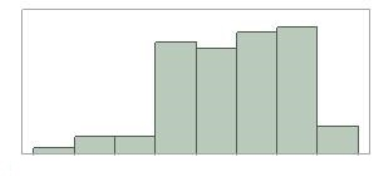
\includegraphics[width=0.98\linewidth]{/Users/lindz/ePort/inst/extdata/KeyFiles/Topic03.Questions_files/image002}\end{marginfigure}\marginnote{

 The values on the horizontal axis are:



a. The number of cars.



*b. The sale prices.



c. The mean sales price for each bin.



d. The mean number of cars for each bin. 

}\vspace{-4cm}\pdfbookmark[2]{T03.C.C.03.1.1.MC.horizontal}{T03.C.C.03.1.1.MC.horizontal} (7) Question "T03.C.C.03.1.1.MC.horizontal" is given on the right. This question was selected from the question set with a frequency of 0.33. The question was administered to 17 out of the total of 50 students. The average score was 0.29 out of 1.

 (Back to the question summary Table \ref{tab:summary_question}.)

\begin{center} \includegraphics[width=.45\linewidth]{Topic03_AB_7_answer} \includegraphics[width=.45\linewidth]{Topic03_AB_7_score} \end{center} 

\begin{center}% latex table generated in R 3.2.2 by xtable 1.8-0 package
% Fri Nov 27 10:29:34 2015
\begin{tabular}{lr}
  \hline
Answer & Count \\ 
  \hline
d &   7 \\ 
  b &   5 \\ 
  a &   4 \\ 
  c &   1 \\ 
   \hline
\end{tabular}
~~~~~~~~% latex table generated in R 3.2.2 by xtable 1.8-0 package
% Fri Nov 27 10:29:34 2015
\begin{tabular}{lr}
  \hline
Summary & Value \\ 
  \hline
Mean & 0.29 \\ 
  Std.dev & 0.47 \\ 
  Min & 0.00 \\ 
  Median & 0.00 \\ 
  Max & 1.00 \\ 
   \hline
\end{tabular}
\end{center}\newpage\marginnote{

 A histogram for the birth weight (in oz.) of a sample of 100 general introductory statistics students is pictured below. 

}



\vspace{4cm}\begin{marginfigure}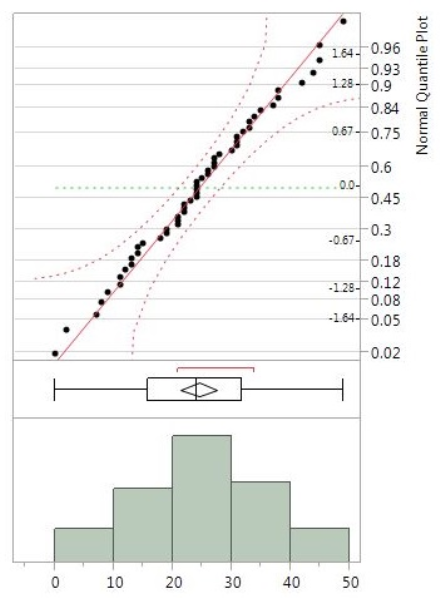
\includegraphics[width=0.98\linewidth]{/Users/lindz/ePort/inst/extdata/KeyFiles/Topic03.Questions_files/image004}\end{marginfigure}\marginnote{

 The values on the horizontal axis are:



a. The number of students.



*b. The birth weights.



c. The mean birth weight for each bin.



d. The mean number of students for each bin. 

}\vspace{-4cm}\pdfbookmark[2]{T03.C.C.03.1.1.MC.horizontal2}{T03.C.C.03.1.1.MC.horizontal2} (8) Question "T03.C.C.03.1.1.MC.horizontal2" is given on the right. This question was selected from the question set with a frequency of 0.33. The question was administered to 16 out of the total of 50 students. The average score was 0.31 out of 1.

 (Back to the question summary Table \ref{tab:summary_question}.)

\begin{center} \includegraphics[width=.45\linewidth]{Topic03_AB_8_answer} \includegraphics[width=.45\linewidth]{Topic03_AB_8_score} \end{center} 

\begin{center}% latex table generated in R 3.2.2 by xtable 1.8-0 package
% Fri Nov 27 10:29:35 2015
\begin{tabular}{lr}
  \hline
Answer & Count \\ 
  \hline
b &   5 \\ 
  c &   4 \\ 
  d &   4 \\ 
  a &   2 \\ 
  Unanswered &   1 \\ 
   \hline
\end{tabular}
~~~~~~~~% latex table generated in R 3.2.2 by xtable 1.8-0 package
% Fri Nov 27 10:29:35 2015
\begin{tabular}{lr}
  \hline
Summary & Value \\ 
  \hline
Mean & 0.31 \\ 
  Std.dev & 0.48 \\ 
  Min & 0.00 \\ 
  Median & 0.00 \\ 
  Max & 1.00 \\ 
   \hline
\end{tabular}
\end{center}\newpage\marginnote{

 A histogram for the number of semester credits hours for a sample of 100 general introductory statistics students is pictured below. 

}



\vspace{5cm}\begin{marginfigure}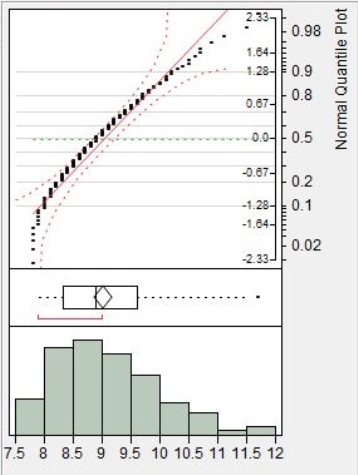
\includegraphics[width=0.98\linewidth]{/Users/lindz/ePort/inst/extdata/KeyFiles/Topic03.Questions_files/image006}\end{marginfigure}\marginnote{

 The values on the horizontal axis are:



a. The number of students.



*b. The number of semester credit hours.



c. The mean number of semester credit hours for each bin.



d. The mean number of students for each bin. 

}\vspace{-5cm}\pdfbookmark[2]{T03.C.C.03.1.1.MC.horizontal3}{T03.C.C.03.1.1.MC.horizontal3} (9) Question "T03.C.C.03.1.1.MC.horizontal3" is given on the right. This question was selected from the question set with a frequency of 0.33. The question was administered to 17 out of the total of 50 students. The average score was 0.53 out of 1.

 (Back to the question summary Table \ref{tab:summary_question}.)

\begin{center} \includegraphics[width=.45\linewidth]{Topic03_AB_9_answer} \includegraphics[width=.45\linewidth]{Topic03_AB_9_score} \end{center} 

\begin{center}% latex table generated in R 3.2.2 by xtable 1.8-0 package
% Fri Nov 27 10:29:35 2015
\begin{tabular}{lr}
  \hline
Answer & Count \\ 
  \hline
b &   9 \\ 
  c &   4 \\ 
  a &   2 \\ 
  d &   2 \\ 
   \hline
\end{tabular}
~~~~~~~~% latex table generated in R 3.2.2 by xtable 1.8-0 package
% Fri Nov 27 10:29:35 2015
\begin{tabular}{lr}
  \hline
Summary & Value \\ 
  \hline
Mean & 0.53 \\ 
  Std.dev & 0.51 \\ 
  Min & 0.00 \\ 
  Median & 1.00 \\ 
  Max & 1.00 \\ 
   \hline
\end{tabular}
\end{center}\newpage\marginnote{

 A histogram for the number of states in the United States visited by a random sample of 100 general introductory statistics students is pictured below. 

}



\vspace{5cm}\begin{marginfigure}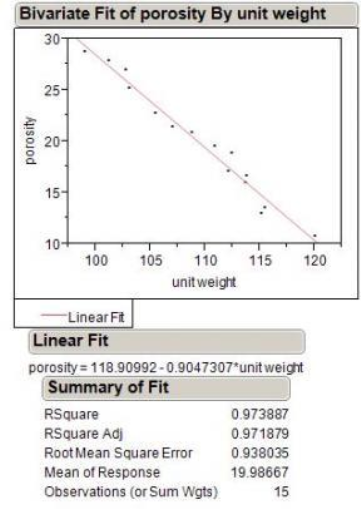
\includegraphics[width=0.98\linewidth]{/Users/lindz/ePort/inst/extdata/KeyFiles/Topic03.Questions_files/image008}\end{marginfigure}\marginnote{

 The values on the vertical axis are:



*a. The number of students.



b. The number of states.



c. The mean number of students for each bin.



d. The mean number of states for each bin. 

}\vspace{-5cm}\pdfbookmark[2]{T03.C.D.03.1.1.MC.vertical}{T03.C.D.03.1.1.MC.vertical} (10) Question "T03.C.D.03.1.1.MC.vertical" is given on the right. This question was selected from the question set with a frequency of 0.33. The question was administered to 21 out of the total of 50 students. The average score was 0.24 out of 1.

 (Back to the question summary Table \ref{tab:summary_question}.)

\begin{center} \includegraphics[width=.45\linewidth]{Topic03_AB_10_answer} \includegraphics[width=.45\linewidth]{Topic03_AB_10_score} \end{center} 

\begin{center}% latex table generated in R 3.2.2 by xtable 1.8-0 package
% Fri Nov 27 10:29:36 2015
\begin{tabular}{lr}
  \hline
Answer & Count \\ 
  \hline
c &   8 \\ 
  a &   5 \\ 
  b &   4 \\ 
  d &   4 \\ 
   \hline
\end{tabular}
~~~~~~~~% latex table generated in R 3.2.2 by xtable 1.8-0 package
% Fri Nov 27 10:29:36 2015
\begin{tabular}{lr}
  \hline
Summary & Value \\ 
  \hline
Mean & 0.24 \\ 
  Std.dev & 0.44 \\ 
  Min & 0.00 \\ 
  Median & 0.00 \\ 
  Max & 1.00 \\ 
   \hline
\end{tabular}
\end{center}\newpage\marginnote{

 A histogram for the population of the 50 states in the United States in 1975 is pictured below. 

}



\vspace{4cm}\begin{marginfigure}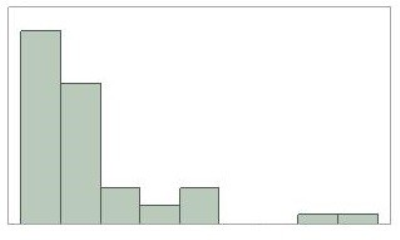
\includegraphics[width=0.98\linewidth]{/Users/lindz/ePort/inst/extdata/KeyFiles/Topic03.Questions_files/image010}\end{marginfigure}\marginnote{

 The values on the vertical axis are:



*a. The number of states.



b. The state population.



c. The mean number of states for each bin.



d. The mean state population for each bin. 

}\vspace{-4cm}\pdfbookmark[2]{T03.C.D.03.1.1.MC.vertical2}{T03.C.D.03.1.1.MC.vertical2} (11) Question "T03.C.D.03.1.1.MC.vertical2" is given on the right. This question was selected from the question set with a frequency of 0.33. The question was administered to 17 out of the total of 50 students. The average score was 0.29 out of 1.

 (Back to the question summary Table \ref{tab:summary_question}.)

\begin{center} \includegraphics[width=.45\linewidth]{Topic03_AB_11_answer} \includegraphics[width=.45\linewidth]{Topic03_AB_11_score} \end{center} 

\begin{center}% latex table generated in R 3.2.2 by xtable 1.8-0 package
% Fri Nov 27 10:29:36 2015
\begin{tabular}{lr}
  \hline
Answer & Count \\ 
  \hline
c &   7 \\ 
  a &   5 \\ 
  b &   2 \\ 
  d &   2 \\ 
  Unanswered &   1 \\ 
   \hline
\end{tabular}
~~~~~~~~% latex table generated in R 3.2.2 by xtable 1.8-0 package
% Fri Nov 27 10:29:36 2015
\begin{tabular}{lr}
  \hline
Summary & Value \\ 
  \hline
Mean & 0.29 \\ 
  Std.dev & 0.47 \\ 
  Min & 0.00 \\ 
  Median & 0.00 \\ 
  Max & 1.00 \\ 
   \hline
\end{tabular}
\end{center}\newpage\marginnote{

 A histogram for the arrival times at the theater before the start of a new movie for 100 people is pictured below. 

}



\vspace{4cm}\begin{marginfigure}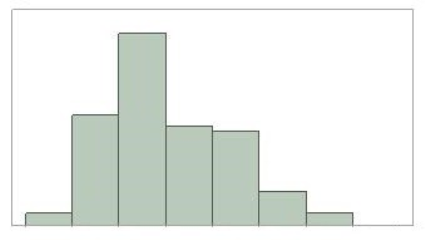
\includegraphics[width=0.98\linewidth]{/Users/lindz/ePort/inst/extdata/KeyFiles/Topic03.Questions_files/image012}\end{marginfigure}\marginnote{

 The values on the vertical axis are:



*a. The number of people.



b. The arrival times.



c. The mean number of people for each bin.



d. The mean arrival times for each bin. 

}\vspace{-4cm}\pdfbookmark[2]{T03.C.D.03.1.1.MC.vertical3}{T03.C.D.03.1.1.MC.vertical3} (12) Question "T03.C.D.03.1.1.MC.vertical3" is given on the right. This question was selected from the question set with a frequency of 0.33. The question was administered to 12 out of the total of 50 students. The average score was 0.17 out of 1.

 (Back to the question summary Table \ref{tab:summary_question}.)

\begin{center} \includegraphics[width=.45\linewidth]{Topic03_AB_12_answer} \includegraphics[width=.45\linewidth]{Topic03_AB_12_score} \end{center} 

\begin{center}% latex table generated in R 3.2.2 by xtable 1.8-0 package
% Fri Nov 27 10:29:37 2015
\begin{tabular}{lr}
  \hline
Answer & Count \\ 
  \hline
c &   7 \\ 
  a &   2 \\ 
  d &   2 \\ 
  b &   1 \\ 
   \hline
\end{tabular}
~~~~~~~~% latex table generated in R 3.2.2 by xtable 1.8-0 package
% Fri Nov 27 10:29:37 2015
\begin{tabular}{lr}
  \hline
Summary & Value \\ 
  \hline
Mean & 0.17 \\ 
  Std.dev & 0.39 \\ 
  Min & 0.00 \\ 
  Median & 0.00 \\ 
  Max & 1.00 \\ 
   \hline
\end{tabular}
\end{center}\newpage\marginnote{

 Below is a histogram of the tips (in dollars) received by a server at a restaurant over a one-week period. 

}



\vspace{4cm}\begin{marginfigure}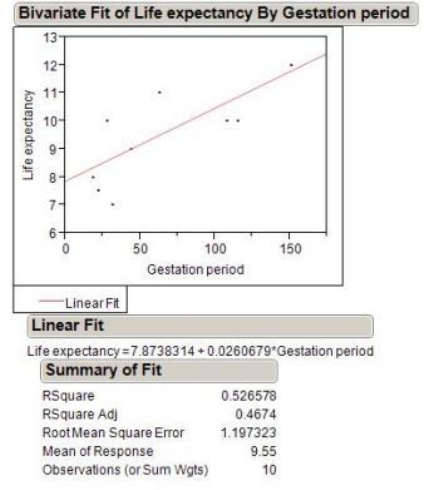
\includegraphics[width=0.98\linewidth]{/Users/lindz/ePort/inst/extdata/KeyFiles/Topic03.Questions_files/image014}\end{marginfigure}\marginnote{

 The tallest bin has a count of 64. This indicates:



a. There were 64 two dollar tips.



b. There were 64 three dollar tips.



c. There were 64 four dollar tips.



*d. There were 64 tips between two and four dollars. 

}\vspace{-4cm}\pdfbookmark[2]{T03.C.E.03.1.1.MC.tips}{T03.C.E.03.1.1.MC.tips} (13) Question "T03.C.E.03.1.1.MC.tips" is given on the right. This question was selected from the question set with a frequency of 0.33. The question was administered to 14 out of the total of 50 students. The average score was 0.36 out of 1.

 (Back to the question summary Table \ref{tab:summary_question}.)

\begin{center} \includegraphics[width=.45\linewidth]{Topic03_AB_13_answer} \includegraphics[width=.45\linewidth]{Topic03_AB_13_score} \end{center} 

\begin{center}% latex table generated in R 3.2.2 by xtable 1.8-0 package
% Fri Nov 27 10:29:37 2015
\begin{tabular}{lr}
  \hline
Answer & Count \\ 
  \hline
d &   5 \\ 
  a &   3 \\ 
  c &   3 \\ 
  b &   2 \\ 
  Unanswered &   1 \\ 
   \hline
\end{tabular}
~~~~~~~~% latex table generated in R 3.2.2 by xtable 1.8-0 package
% Fri Nov 27 10:29:37 2015
\begin{tabular}{lr}
  \hline
Summary & Value \\ 
  \hline
Mean & 0.36 \\ 
  Std.dev & 0.50 \\ 
  Min & 0.00 \\ 
  Median & 0.00 \\ 
  Max & 1.00 \\ 
   \hline
\end{tabular}
\end{center}\newpage\marginnote{

 Below is a histogram of the tips (in dollars) received by a server at a restaurant over a one-week period. 

}



\vspace{4cm}\begin{marginfigure}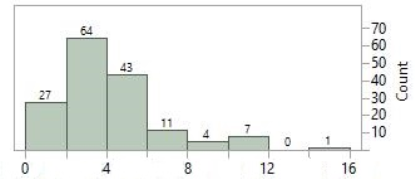
\includegraphics[width=0.98\linewidth]{/Users/lindz/ePort/inst/extdata/KeyFiles/Topic03.Questions_files/image015}\end{marginfigure}\marginnote{

 The second tallest bin has a count of 43. This indicates:



a. There were 43 four dollar tips.



b. There were 43 five dollar tips.



c. There were 43 six dollar tips.



*d. There were 43 tips between four and six dollars. 

}\vspace{-4cm}\pdfbookmark[2]{T03.C.E.03.1.1.MC.tips2}{T03.C.E.03.1.1.MC.tips2} (14) Question "T03.C.E.03.1.1.MC.tips2" is given on the right. This question was selected from the question set with a frequency of 0.33. The question was administered to 15 out of the total of 50 students. The average score was 0.33 out of 1.

 (Back to the question summary Table \ref{tab:summary_question}.)

\begin{center} \includegraphics[width=.45\linewidth]{Topic03_AB_14_answer} \includegraphics[width=.45\linewidth]{Topic03_AB_14_score} \end{center} 

\begin{center}% latex table generated in R 3.2.2 by xtable 1.8-0 package
% Fri Nov 27 10:29:38 2015
\begin{tabular}{lr}
  \hline
Answer & Count \\ 
  \hline
d &   5 \\ 
  a &   4 \\ 
  c &   4 \\ 
  b &   2 \\ 
   \hline
\end{tabular}
~~~~~~~~% latex table generated in R 3.2.2 by xtable 1.8-0 package
% Fri Nov 27 10:29:38 2015
\begin{tabular}{lr}
  \hline
Summary & Value \\ 
  \hline
Mean & 0.33 \\ 
  Std.dev & 0.49 \\ 
  Min & 0.00 \\ 
  Median & 0.00 \\ 
  Max & 1.00 \\ 
   \hline
\end{tabular}
\end{center}\newpage\marginnote{

 Below is a histogram of the tips (in dollars) received by a server at a restaurant over a one-week period. 

}



\vspace{4cm}\begin{marginfigure}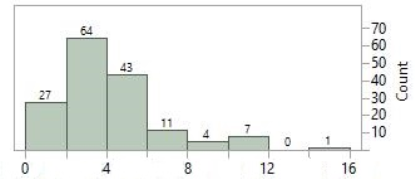
\includegraphics[width=0.98\linewidth]{/Users/lindz/ePort/inst/extdata/KeyFiles/Topic03.Questions_files/image015}\end{marginfigure}\marginnote{

 The fourth tallest bin has a count of 11. This indicates:



a. There were 11 six dollar tips.



b. There were 11 seven dollar tips.



c. There were 11 eight dollar tips.



*d. There were 11 tips between six and eight dollars. 

}\vspace{-4cm}\pdfbookmark[2]{T03.C.E.03.1.1.MC.tips3}{T03.C.E.03.1.1.MC.tips3} (15) Question "T03.C.E.03.1.1.MC.tips3" is given on the right. This question was selected from the question set with a frequency of 0.33. The question was administered to 21 out of the total of 50 students. The average score was 0.33 out of 1.

 (Back to the question summary Table \ref{tab:summary_question}.)

\begin{center} \includegraphics[width=.45\linewidth]{Topic03_AB_15_answer} \includegraphics[width=.45\linewidth]{Topic03_AB_15_score} \end{center} 

\begin{center}% latex table generated in R 3.2.2 by xtable 1.8-0 package
% Fri Nov 27 10:29:38 2015
\begin{tabular}{lr}
  \hline
Answer & Count \\ 
  \hline
d &   7 \\ 
  a &   6 \\ 
  c &   6 \\ 
  b &   2 \\ 
   \hline
\end{tabular}
~~~~~~~~% latex table generated in R 3.2.2 by xtable 1.8-0 package
% Fri Nov 27 10:29:38 2015
\begin{tabular}{lr}
  \hline
Summary & Value \\ 
  \hline
Mean & 0.33 \\ 
  Std.dev & 0.48 \\ 
  Min & 0.00 \\ 
  Median & 0.00 \\ 
  Max & 1.00 \\ 
   \hline
\end{tabular}
\end{center}\newpage\marginnote{

 Below is a histogram for arrival delays of flights for an airline. 

}



\vspace{4cm}\begin{marginfigure}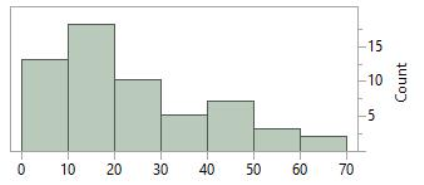
\includegraphics[width=0.98\linewidth]{/Users/lindz/ePort/inst/extdata/KeyFiles/Topic03.Questions_files/image017}\end{marginfigure}\marginnote{

 How many flights were delayed between 20 and 30 minutes?



a. 18



b. 13



*c. 10



d. 5 

}\vspace{-4cm}\pdfbookmark[2]{T03.C.F.04.1.1.MC.flights1}{T03.C.F.04.1.1.MC.flights1} (16) Question "T03.C.F.04.1.1.MC.flights1" is given on the right. This question was selected from the question set with a frequency of 0.25. The question was administered to 16 out of the total of 50 students. The average score was 0.31 out of 1.

 (Back to the question summary Table \ref{tab:summary_question}.)

\begin{center} \includegraphics[width=.45\linewidth]{Topic03_AB_16_answer} \includegraphics[width=.45\linewidth]{Topic03_AB_16_score} \end{center} 

\begin{center}% latex table generated in R 3.2.2 by xtable 1.8-0 package
% Fri Nov 27 10:29:39 2015
\begin{tabular}{lr}
  \hline
Answer & Count \\ 
  \hline
b &   6 \\ 
  c &   5 \\ 
  d &   3 \\ 
  a &   2 \\ 
   \hline
\end{tabular}
~~~~~~~~% latex table generated in R 3.2.2 by xtable 1.8-0 package
% Fri Nov 27 10:29:39 2015
\begin{tabular}{lr}
  \hline
Summary & Value \\ 
  \hline
Mean & 0.31 \\ 
  Std.dev & 0.48 \\ 
  Min & 0.00 \\ 
  Median & 0.00 \\ 
  Max & 1.00 \\ 
   \hline
\end{tabular}
\end{center}\newpage\marginnote{

 Below is a histogram for arrival delays of flights for an airline. 

}



\vspace{4cm}\begin{marginfigure}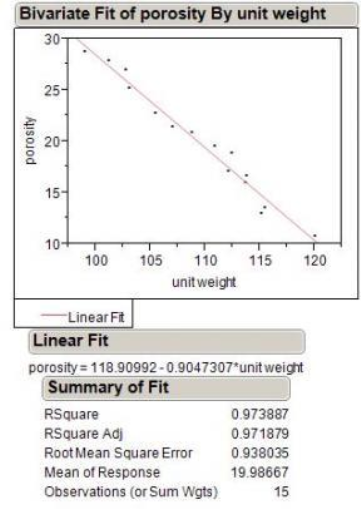
\includegraphics[width=0.98\linewidth]{/Users/lindz/ePort/inst/extdata/KeyFiles/Topic03.Questions_files/image018}\end{marginfigure}\marginnote{

 How many flights were delayed between 10 and 20 minutes?



*a. 18



b. 13



c. 10



d. 5 

}\vspace{-4cm}\pdfbookmark[2]{T03.C.F.04.1.1.MC.flights2}{T03.C.F.04.1.1.MC.flights2} (17) Question "T03.C.F.04.1.1.MC.flights2" is given on the right. This question was selected from the question set with a frequency of 0.25. The question was administered to 13 out of the total of 50 students. The average score was 0.31 out of 1.

 (Back to the question summary Table \ref{tab:summary_question}.)

\begin{center} \includegraphics[width=.45\linewidth]{Topic03_AB_17_answer} \includegraphics[width=.45\linewidth]{Topic03_AB_17_score} \end{center} 

\begin{center}% latex table generated in R 3.2.2 by xtable 1.8-0 package
% Fri Nov 27 10:29:39 2015
\begin{tabular}{lr}
  \hline
Answer & Count \\ 
  \hline
d &   6 \\ 
  a &   4 \\ 
  b &   2 \\ 
  c &   1 \\ 
   \hline
\end{tabular}
~~~~~~~~% latex table generated in R 3.2.2 by xtable 1.8-0 package
% Fri Nov 27 10:29:40 2015
\begin{tabular}{lr}
  \hline
Summary & Value \\ 
  \hline
Mean & 0.31 \\ 
  Std.dev & 0.48 \\ 
  Min & 0.00 \\ 
  Median & 0.00 \\ 
  Max & 1.00 \\ 
   \hline
\end{tabular}
\end{center}\newpage\marginnote{

 Below is a histogram for arrival delays of flights for an airline. 

}



\vspace{4cm}\begin{marginfigure}\includegraphics[width=0.98\linewidth]{/Users/lindz/ePort/inst/extdata/KeyFiles/Topic03.Questions_files/image019}\end{marginfigure}\marginnote{

 How many flights were delayed between 30 and 40 minutes?



a. 18



b. 13



c. 10



*d. 5 

}\vspace{-4cm}\pdfbookmark[2]{T03.C.F.04.1.1.MC.flights3}{T03.C.F.04.1.1.MC.flights3} (18) Question "T03.C.F.04.1.1.MC.flights3" is given on the right. This question was selected from the question set with a frequency of 0.25. The question was administered to 9 out of the total of 50 students. The average score was 0.22 out of 1.

 (Back to the question summary Table \ref{tab:summary_question}.)

\begin{center} \includegraphics[width=.45\linewidth]{Topic03_AB_18_answer} \includegraphics[width=.45\linewidth]{Topic03_AB_18_score} \end{center} 

\begin{center}% latex table generated in R 3.2.2 by xtable 1.8-0 package
% Fri Nov 27 10:29:40 2015
\begin{tabular}{lr}
  \hline
Answer & Count \\ 
  \hline
a &   3 \\ 
  c &   2 \\ 
  d &   2 \\ 
  b &   1 \\ 
  Unanswered &   1 \\ 
   \hline
\end{tabular}
~~~~~~~~% latex table generated in R 3.2.2 by xtable 1.8-0 package
% Fri Nov 27 10:29:40 2015
\begin{tabular}{lr}
  \hline
Summary & Value \\ 
  \hline
Mean & 0.22 \\ 
  Std.dev & 0.44 \\ 
  Min & 0.00 \\ 
  Median & 0.00 \\ 
  Max & 1.00 \\ 
   \hline
\end{tabular}
\end{center}\newpage\marginnote{

 Below is a histogram for arrival delays of flights for an airline. 

}



\vspace{4cm}\begin{marginfigure}\includegraphics[width=0.98\linewidth]{/Users/lindz/ePort/inst/extdata/KeyFiles/Topic03.Questions_files/image020}\end{marginfigure}\marginnote{

 How many flights were delayed between 0 and 10 minutes?



a. 18



*b. 13



c. 10



d. 5 

}\vspace{-4cm}\pdfbookmark[2]{T03.C.F.04.1.1.MC.flights4}{T03.C.F.04.1.1.MC.flights4} (19) Question "T03.C.F.04.1.1.MC.flights4" is given on the right. This question was selected from the question set with a frequency of 0.25. The question was administered to 12 out of the total of 50 students. The average score was 0.25 out of 1.

 (Back to the question summary Table \ref{tab:summary_question}.)

\begin{center} \includegraphics[width=.45\linewidth]{Topic03_AB_19_answer} \includegraphics[width=.45\linewidth]{Topic03_AB_19_score} \end{center} 

\begin{center}% latex table generated in R 3.2.2 by xtable 1.8-0 package
% Fri Nov 27 10:29:40 2015
\begin{tabular}{lr}
  \hline
Answer & Count \\ 
  \hline
c &   4 \\ 
  b &   3 \\ 
  d &   3 \\ 
  a &   2 \\ 
   \hline
\end{tabular}
~~~~~~~~% latex table generated in R 3.2.2 by xtable 1.8-0 package
% Fri Nov 27 10:29:41 2015
\begin{tabular}{lr}
  \hline
Summary & Value \\ 
  \hline
Mean & 0.25 \\ 
  Std.dev & 0.45 \\ 
  Min & 0.00 \\ 
  Median & 0.00 \\ 
  Max & 1.00 \\ 
   \hline
\end{tabular}
\end{center}\newpage\marginnote{

 Below is a histogram for arrival delays of flights for an airline. 

}



\vspace{4cm}\begin{marginfigure}\includegraphics[width=0.98\linewidth]{/Users/lindz/ePort/inst/extdata/KeyFiles/Topic03.Questions_files/image021}\end{marginfigure}\marginnote{

 How many flights were delayed between 0 and 20 minutes?



*a. 31



b. 28



c. 15



d. 12 

}\vspace{-4cm}\pdfbookmark[2]{T03.C.G.04.1.1.MC.flights5}{T03.C.G.04.1.1.MC.flights5} (20) Question "T03.C.G.04.1.1.MC.flights5" is given on the right. This question was selected from the question set with a frequency of 0.25. The question was administered to 13 out of the total of 50 students. The average score was 0.15 out of 1.

 (Back to the question summary Table \ref{tab:summary_question}.)

\begin{center} \includegraphics[width=.45\linewidth]{Topic03_AB_20_answer} \includegraphics[width=.45\linewidth]{Topic03_AB_20_score} \end{center} 

\begin{center}% latex table generated in R 3.2.2 by xtable 1.8-0 package
% Fri Nov 27 10:29:41 2015
\begin{tabular}{lr}
  \hline
Answer & Count \\ 
  \hline
c &   4 \\ 
  d &   4 \\ 
  b &   3 \\ 
  a &   2 \\ 
   \hline
\end{tabular}
~~~~~~~~% latex table generated in R 3.2.2 by xtable 1.8-0 package
% Fri Nov 27 10:29:41 2015
\begin{tabular}{lr}
  \hline
Summary & Value \\ 
  \hline
Mean & 0.15 \\ 
  Std.dev & 0.38 \\ 
  Min & 0.00 \\ 
  Median & 0.00 \\ 
  Max & 1.00 \\ 
   \hline
\end{tabular}
\end{center}\newpage\marginnote{

 Below is a histogram for arrival delays of flights for an airline. 

}



\vspace{4cm}\begin{marginfigure}\includegraphics[width=0.98\linewidth]{/Users/lindz/ePort/inst/extdata/KeyFiles/Topic03.Questions_files/image019}\end{marginfigure}\marginnote{

 How many flights were delayed between 10 and 30 minutes?



a. 31



*b. 28



c. 15



d. 12 

}\vspace{-4cm}\pdfbookmark[2]{T03.C.G.04.1.1.MC.flights6}{T03.C.G.04.1.1.MC.flights6} (21) Question "T03.C.G.04.1.1.MC.flights6" is given on the right. This question was selected from the question set with a frequency of 0.25. The question was administered to 10 out of the total of 50 students. The average score was 0.2 out of 1.

 (Back to the question summary Table \ref{tab:summary_question}.)

\begin{center} \includegraphics[width=.45\linewidth]{Topic03_AB_21_answer} \includegraphics[width=.45\linewidth]{Topic03_AB_21_score} \end{center} 

\begin{center}% latex table generated in R 3.2.2 by xtable 1.8-0 package
% Fri Nov 27 10:29:41 2015
\begin{tabular}{lr}
  \hline
Answer & Count \\ 
  \hline
a &   3 \\ 
  c &   3 \\ 
  b &   2 \\ 
  d &   1 \\ 
  Unanswered &   1 \\ 
   \hline
\end{tabular}
~~~~~~~~% latex table generated in R 3.2.2 by xtable 1.8-0 package
% Fri Nov 27 10:29:42 2015
\begin{tabular}{lr}
  \hline
Summary & Value \\ 
  \hline
Mean & 0.20 \\ 
  Std.dev & 0.42 \\ 
  Min & 0.00 \\ 
  Median & 0.00 \\ 
  Max & 1.00 \\ 
   \hline
\end{tabular}
\end{center}\newpage\marginnote{

 Below is a histogram for arrival delays of flights for an airline. 

}



\vspace{4cm}\begin{marginfigure}\includegraphics[width=0.98\linewidth]{/Users/lindz/ePort/inst/extdata/KeyFiles/Topic03.Questions_files/image021}\end{marginfigure}\marginnote{

 How many flights were delayed between 20 and 40 minutes?



a. 31



b. 28



*c. 15



d. 12 

}\vspace{-4cm}\pdfbookmark[2]{T03.C.G.04.1.1.MC.flights7}{T03.C.G.04.1.1.MC.flights7} (22) Question "T03.C.G.04.1.1.MC.flights7" is given on the right. This question was selected from the question set with a frequency of 0.25. The question was administered to 12 out of the total of 50 students. The average score was 0.08 out of 1.

 (Back to the question summary Table \ref{tab:summary_question}.)

\begin{center} \includegraphics[width=.45\linewidth]{Topic03_AB_22_answer} \includegraphics[width=.45\linewidth]{Topic03_AB_22_score} \end{center} 

\begin{center}% latex table generated in R 3.2.2 by xtable 1.8-0 package
% Fri Nov 27 10:29:42 2015
\begin{tabular}{lr}
  \hline
Answer & Count \\ 
  \hline
b &   5 \\ 
  a &   4 \\ 
  d &   2 \\ 
  c &   1 \\ 
   \hline
\end{tabular}
~~~~~~~~% latex table generated in R 3.2.2 by xtable 1.8-0 package
% Fri Nov 27 10:29:42 2015
\begin{tabular}{lr}
  \hline
Summary & Value \\ 
  \hline
Mean & 0.08 \\ 
  Std.dev & 0.29 \\ 
  Min & 0.00 \\ 
  Median & 0.00 \\ 
  Max & 1.00 \\ 
   \hline
\end{tabular}
\end{center}\newpage\marginnote{

 Below is a histogram for arrival delays of flights for an airline. 

}



\vspace{4cm}\begin{marginfigure}\includegraphics[width=0.98\linewidth]{/Users/lindz/ePort/inst/extdata/KeyFiles/Topic03.Questions_files/image021}\end{marginfigure}\marginnote{

 How many flights were delayed between 30 and 50 minutes?



a. 31



b. 28



c. 15



*d. 12 

}\vspace{-4cm}\pdfbookmark[2]{T03.C.G.04.1.1.MC.flights8}{T03.C.G.04.1.1.MC.flights8} (23) Question "T03.C.G.04.1.1.MC.flights8" is given on the right. This question was selected from the question set with a frequency of 0.25. The question was administered to 15 out of the total of 50 students. The average score was 0.33 out of 1.

 (Back to the question summary Table \ref{tab:summary_question}.)

\begin{center} \includegraphics[width=.45\linewidth]{Topic03_AB_23_answer} \includegraphics[width=.45\linewidth]{Topic03_AB_23_score} \end{center} 

\begin{center}% latex table generated in R 3.2.2 by xtable 1.8-0 package
% Fri Nov 27 10:29:43 2015
\begin{tabular}{lr}
  \hline
Answer & Count \\ 
  \hline
a &   5 \\ 
  d &   5 \\ 
  b &   4 \\ 
  c &   1 \\ 
   \hline
\end{tabular}
~~~~~~~~% latex table generated in R 3.2.2 by xtable 1.8-0 package
% Fri Nov 27 10:29:43 2015
\begin{tabular}{lr}
  \hline
Summary & Value \\ 
  \hline
Mean & 0.33 \\ 
  Std.dev & 0.49 \\ 
  Min & 0.00 \\ 
  Median & 0.00 \\ 
  Max & 1.00 \\ 
   \hline
\end{tabular}
\end{center}\newpage\marginnote{

 Which of the following best describes the shape of the distribution pictured below? 

}



\vspace{4cm}\begin{marginfigure}\includegraphics[width=0.98\linewidth]{/Users/lindz/ePort/inst/extdata/KeyFiles/Topic03.Questions_files/image023}\end{marginfigure}\marginnote{

 *a. Uniform



b. Symmetric and unimodal



c. Skewed left and unimodal



d. Skewed left and bimodal



e. Skewed right and unimodal



f. Skewed right and bimodal 

}\vspace{-4cm}\pdfbookmark[2]{T03.D.H.04.2.1.MC.random1}{T03.D.H.04.2.1.MC.random1} (24) Question "T03.D.H.04.2.1.MC.random1" is given on the right. This question was selected from the question set with a frequency of 0.5. The question was administered to 29 out of the total of 50 students. The average score was 0.31 out of 1.

 (Back to the question summary Table \ref{tab:summary_question}.)

\begin{center} \includegraphics[width=.45\linewidth]{Topic03_AB_24_answer} \includegraphics[width=.45\linewidth]{Topic03_AB_24_score} \end{center} 

\begin{center}% latex table generated in R 3.2.2 by xtable 1.8-0 package
% Fri Nov 27 10:29:43 2015
\begin{tabular}{lr}
  \hline
Answer & Count \\ 
  \hline
a &   9 \\ 
  e &   6 \\ 
  c &   4 \\ 
  f &   4 \\ 
  b &   3 \\ 
  d &   2 \\ 
  Unanswered &   1 \\ 
   \hline
\end{tabular}
~~~~~~~~% latex table generated in R 3.2.2 by xtable 1.8-0 package
% Fri Nov 27 10:29:43 2015
\begin{tabular}{lr}
  \hline
Summary & Value \\ 
  \hline
Mean & 0.31 \\ 
  Std.dev & 0.47 \\ 
  Min & 0.00 \\ 
  Median & 0.00 \\ 
  Max & 1.00 \\ 
   \hline
\end{tabular}
\end{center}\newpage\marginnote{

 Which of the following best describes the shape of the distribution pictured below? 

}



\vspace{4cm}\begin{marginfigure}\includegraphics[width=0.98\linewidth]{/Users/lindz/ePort/inst/extdata/KeyFiles/Topic03.Questions_files/image025}\end{marginfigure}\marginnote{

 a. Uniform



b. Symmetric and unimodal



*c. Skewed left and unimodal



d. Skewed left and bimodal



e. Skewed right and unimodal



f. Skewed right and bimodal 

}\vspace{-4cm}\pdfbookmark[2]{T03.D.H.04.2.1.MC.random2}{T03.D.H.04.2.1.MC.random2} (25) Question "T03.D.H.04.2.1.MC.random2" is given on the right. This question was selected from the question set with a frequency of 0.5. The question was administered to 23 out of the total of 50 students. The average score was 0.39 out of 1.

 (Back to the question summary Table \ref{tab:summary_question}.)

\begin{center} \includegraphics[width=.45\linewidth]{Topic03_AB_25_answer} \includegraphics[width=.45\linewidth]{Topic03_AB_25_score} \end{center} 

\begin{center}% latex table generated in R 3.2.2 by xtable 1.8-0 package
% Fri Nov 27 10:29:44 2015
\begin{tabular}{lr}
  \hline
Answer & Count \\ 
  \hline
c &   9 \\ 
  a &   4 \\ 
  d &   4 \\ 
  b &   3 \\ 
  e &   2 \\ 
  f &   1 \\ 
   \hline
\end{tabular}
~~~~~~~~% latex table generated in R 3.2.2 by xtable 1.8-0 package
% Fri Nov 27 10:29:44 2015
\begin{tabular}{lr}
  \hline
Summary & Value \\ 
  \hline
Mean & 0.39 \\ 
  Std.dev & 0.50 \\ 
  Min & 0.00 \\ 
  Median & 0.00 \\ 
  Max & 1.00 \\ 
   \hline
\end{tabular}
\end{center}\newpage\marginnote{

 Which of the following best describes the shape of the distribution pictured below? 

}



\vspace{4cm}\begin{marginfigure}\includegraphics[width=0.98\linewidth]{/Users/lindz/ePort/inst/extdata/KeyFiles/Topic03.Questions_files/image027}\end{marginfigure}\marginnote{

 a. Uniform



*b. Symmetric and unimodal



c. Skewed left and unimodal



d. Skewed left and bimodal



e. Skewed right and unimodal



f. Skewed right and bimodal 

}\vspace{-4cm}\pdfbookmark[2]{T03.D.H.04.2.1.MC.random3}{T03.D.H.04.2.1.MC.random3} (26) Question "T03.D.H.04.2.1.MC.random3" is given on the right. This question was selected from the question set with a frequency of 0.5. The question was administered to 26 out of the total of 50 students. The average score was 0.23 out of 1.

 (Back to the question summary Table \ref{tab:summary_question}.)

\begin{center} \includegraphics[width=.45\linewidth]{Topic03_AB_26_answer} \includegraphics[width=.45\linewidth]{Topic03_AB_26_score} \end{center} 

\begin{center}% latex table generated in R 3.2.2 by xtable 1.8-0 package
% Fri Nov 27 10:29:44 2015
\begin{tabular}{lr}
  \hline
Answer & Count \\ 
  \hline
b &   6 \\ 
  e &   6 \\ 
  d &   4 \\ 
  f &   4 \\ 
  a &   3 \\ 
  c &   2 \\ 
  Unanswered &   1 \\ 
   \hline
\end{tabular}
~~~~~~~~% latex table generated in R 3.2.2 by xtable 1.8-0 package
% Fri Nov 27 10:29:44 2015
\begin{tabular}{lr}
  \hline
Summary & Value \\ 
  \hline
Mean & 0.23 \\ 
  Std.dev & 0.43 \\ 
  Min & 0.00 \\ 
  Median & 0.00 \\ 
  Max & 1.00 \\ 
   \hline
\end{tabular}
\end{center}\newpage\marginnote{

 Which of the following best describes the shape of the distribution pictured below? 

}



\vspace{4cm}\begin{marginfigure}\includegraphics[width=0.98\linewidth]{/Users/lindz/ePort/inst/extdata/KeyFiles/Topic03.Questions_files/image029}\end{marginfigure}\marginnote{

 a. Uniform



b. Symmetric and unimodal



c. Skewed left and unimodal



d. Skewed left and bimodal



*e. Skewed right and unimodal



f. Skewed right and bimodal 

}\vspace{-4cm}\pdfbookmark[2]{T03.D.H.04.2.1.MC.random4}{T03.D.H.04.2.1.MC.random4} (27) Question "T03.D.H.04.2.1.MC.random4" is given on the right. This question was selected from the question set with a frequency of 0.5. The question was administered to 22 out of the total of 50 students. The average score was 0.27 out of 1.

 (Back to the question summary Table \ref{tab:summary_question}.)

\begin{center} \includegraphics[width=.45\linewidth]{Topic03_AB_27_answer} \includegraphics[width=.45\linewidth]{Topic03_AB_27_score} \end{center} 

\begin{center}% latex table generated in R 3.2.2 by xtable 1.8-0 package
% Fri Nov 27 10:29:45 2015
\begin{tabular}{lr}
  \hline
Answer & Count \\ 
  \hline
b &   7 \\ 
  e &   6 \\ 
  d &   3 \\ 
  f &   3 \\ 
  c &   2 \\ 
  a &   1 \\ 
   \hline
\end{tabular}
~~~~~~~~% latex table generated in R 3.2.2 by xtable 1.8-0 package
% Fri Nov 27 10:29:45 2015
\begin{tabular}{lr}
  \hline
Summary & Value \\ 
  \hline
Mean & 0.27 \\ 
  Std.dev & 0.46 \\ 
  Min & 0.00 \\ 
  Median & 0.00 \\ 
  Max & 1.00 \\ 
   \hline
\end{tabular}
\end{center}\newpage\marginnote{

 A blowhole is a hole in a cliff that produces eruptions of water when the ocean swell hits the cliff. Below is the histogram and stem-and-leaf plot for 40 times (in seconds) between eruptions for the Kiama blowhole in Australia. 

}



\vspace{5cm}\begin{marginfigure}\includegraphics[width=0.98\linewidth]{/Users/lindz/ePort/inst/extdata/KeyFiles/Topic03.Questions_files/image031}\end{marginfigure}\marginnote{

 Which of the following statements does NOT describe the distribution of time between eruptions?



a. There are 24 observations where the time between eruptions is less than 30 seconds.



b. The distribution of the times between eruptions is skewed to the right.



c. The mean time between eruptions is greater than the median time between eruptions.



d. The minimum time between eruptions is 7 seconds.



*e. The median time between eruptions is less than 20 seconds. 

}\vspace{-5cm}\pdfbookmark[2]{T03.E.I.06.3.1.MC.blowhole}{T03.E.I.06.3.1.MC.blowhole} (28) Question "T03.E.I.06.3.1.MC.blowhole" is given on the right. This question was selected from the question set with a frequency of 0.5. The question was administered to 22 out of the total of 50 students. The average score was 0.14 out of 1.

 (Back to the question summary Table \ref{tab:summary_question}.)

\begin{center} \includegraphics[width=.45\linewidth]{Topic03_AB_28_answer} \includegraphics[width=.45\linewidth]{Topic03_AB_28_score} \end{center} 

\begin{center}% latex table generated in R 3.2.2 by xtable 1.8-0 package
% Fri Nov 27 10:29:46 2015
\begin{tabular}{lr}
  \hline
Answer & Count \\ 
  \hline
d &   6 \\ 
  a &   5 \\ 
  b &   5 \\ 
  c &   3 \\ 
  e &   3 \\ 
   \hline
\end{tabular}
~~~~~~~~% latex table generated in R 3.2.2 by xtable 1.8-0 package
% Fri Nov 27 10:29:46 2015
\begin{tabular}{lr}
  \hline
Summary & Value \\ 
  \hline
Mean & 0.14 \\ 
  Std.dev & 0.35 \\ 
  Min & 0.00 \\ 
  Median & 0.00 \\ 
  Max & 1.00 \\ 
   \hline
\end{tabular}
\end{center}\newpage\marginnote{

 Data are obtained on the forced expiratory volume (FEV) of youths in East Boston in the late 1970s. Forced expiratory volume (FEV) is a measure of lung capacity, in liters. The initial measurements in the 1970s provide a baseline value to study the impact of smoking on lung function. The data for this problem are a random sample of 100 FEV values. 

}



\vspace{6cm}\begin{marginfigure}\includegraphics[width=0.98\linewidth]{/Users/lindz/ePort/inst/extdata/KeyFiles/Topic03.Questions_files/image033}\end{marginfigure}\marginnote{

 Which of the following statements does NOT describe the distribution of FEV values?



a. The distribution of FEV values is slightly skewed to the right.



b. The distribution of FEV values is unimodal.



c. The center of the FEV values is between 2.0 and 2.5.



d. The range of the FEV values is from 0.8 to 4.7.



*e. The mean FEV value will be less than the median FEV value. 

}\vspace{-6cm}\pdfbookmark[2]{T03.E.I.06.3.1.MC.FEV}{T03.E.I.06.3.1.MC.FEV} (29) Question "T03.E.I.06.3.1.MC.FEV" is given on the right. This question was selected from the question set with a frequency of 0.5. The question was administered to 26 out of the total of 50 students. The average score was 0.19 out of 1.

 (Back to the question summary Table \ref{tab:summary_question}.)

\begin{center} \includegraphics[width=.45\linewidth]{Topic03_AB_29_answer} \includegraphics[width=.45\linewidth]{Topic03_AB_29_score} \end{center} 

\begin{center}% latex table generated in R 3.2.2 by xtable 1.8-0 package
% Fri Nov 27 10:29:46 2015
\begin{tabular}{lr}
  \hline
Answer & Count \\ 
  \hline
b &   8 \\ 
  d &   5 \\ 
  e &   5 \\ 
  a &   4 \\ 
  c &   4 \\ 
   \hline
\end{tabular}
~~~~~~~~% latex table generated in R 3.2.2 by xtable 1.8-0 package
% Fri Nov 27 10:29:46 2015
\begin{tabular}{lr}
  \hline
Summary & Value \\ 
  \hline
Mean & 0.19 \\ 
  Std.dev & 0.40 \\ 
  Min & 0.00 \\ 
  Median & 0.00 \\ 
  Max & 1.00 \\ 
   \hline
\end{tabular}
\end{center}\newpage\marginnote{

 The sizes of diamonds (in carats) in 48 ladies diamond rings were recorded and the data are shown below. 

}



\vspace{4cm}\begin{marginfigure}\includegraphics[width=0.98\linewidth]{/Users/lindz/ePort/inst/extdata/KeyFiles/Topic03.Questions_files/image035}\end{marginfigure}\marginnote{

 Which of the following statements does NOT describe the distribution of diamond size?



a. The distribution of diamond size is skewed to the right.



b. The mean diamond size will be greater than the median diamond size.



c. The distribution of diamond size is bimodal with the larger mode between 0.15 to 0.2 carats and a smaller mode between 0.25 and 0.3 carats.



d. There are 29 diamonds smaller than 0.2 carats in size.



*e. The distribution of diamond size is unimodal with one mode between 0.15 and 0.2 carats. 

}\vspace{-4cm}\pdfbookmark[2]{T03.E.I.06.3.1.MC.diamonds}{T03.E.I.06.3.1.MC.diamonds} (30) Question "T03.E.I.06.3.1.MC.diamonds" is given on the right. This question was selected from the question set with a frequency of 0.5. The question was administered to 26 out of the total of 50 students. The average score was 0.15 out of 1.

 (Back to the question summary Table \ref{tab:summary_question}.)

\begin{center} \includegraphics[width=.45\linewidth]{Topic03_AB_30_answer} \includegraphics[width=.45\linewidth]{Topic03_AB_30_score} \end{center} 

\begin{center}% latex table generated in R 3.2.2 by xtable 1.8-0 package
% Fri Nov 27 10:29:47 2015
\begin{tabular}{lr}
  \hline
Answer & Count \\ 
  \hline
b &   8 \\ 
  c &   8 \\ 
  a &   4 \\ 
  e &   4 \\ 
  d &   2 \\ 
   \hline
\end{tabular}
~~~~~~~~% latex table generated in R 3.2.2 by xtable 1.8-0 package
% Fri Nov 27 10:29:47 2015
\begin{tabular}{lr}
  \hline
Summary & Value \\ 
  \hline
Mean & 0.15 \\ 
  Std.dev & 0.37 \\ 
  Min & 0.00 \\ 
  Median & 0.00 \\ 
  Max & 1.00 \\ 
   \hline
\end{tabular}
\end{center}\newpage\marginnote{

 A telecommunications equipment manufacturer was receiving complaints about low volume on long distance calls. Amplifiers are used to boost the signal at various points in the long distance lines. The boosting ability of the amplifiers is called “gain.” Amplifiers are designed to have a gain of 10 decibels (dB). This means that a 1 dB input signal would be boosted to a 10 dB output signal. A sample of 120 amplifiers is tested for gain. 

}



\vspace{7cm}\begin{marginfigure}\includegraphics[width=0.98\linewidth]{/Users/lindz/ePort/inst/extdata/KeyFiles/Topic03.Questions_files/image037}\end{marginfigure}\marginnote{

 Which of the following statements does NOT describe the distribution of gain values?



*a. The distribution of amplifier gain values is skewed to the left.



b. The center of amplifier gain values is around 9 dB.



c. The range of amplifier gain values is from 7.8 dB to 11.7 dB.



d. The mean amplifier gain value will be greater than the median amplifier gain value.



e. The distribution of amplifier gain values is unimodal with the mode between 8.5 dB and 9.0 dB. 

}\vspace{-7cm}\pdfbookmark[2]{T03.E.I.06.3.1.MC.amps}{T03.E.I.06.3.1.MC.amps} (31) Question "T03.E.I.06.3.1.MC.amps" is given on the right. This question was selected from the question set with a frequency of 0.5. The question was administered to 30 out of the total of 50 students. The average score was 0.23 out of 1.

 (Back to the question summary Table \ref{tab:summary_question}.)

\begin{center} \includegraphics[width=.45\linewidth]{Topic03_AB_31_answer} \includegraphics[width=.45\linewidth]{Topic03_AB_31_score} \end{center} 

\begin{center}% latex table generated in R 3.2.2 by xtable 1.8-0 package
% Fri Nov 27 10:29:47 2015
\begin{tabular}{lr}
  \hline
Answer & Count \\ 
  \hline
b &   8 \\ 
  a &   7 \\ 
  d &   5 \\ 
  e &   5 \\ 
  c &   4 \\ 
  Unanswered &   1 \\ 
   \hline
\end{tabular}
~~~~~~~~% latex table generated in R 3.2.2 by xtable 1.8-0 package
% Fri Nov 27 10:29:47 2015
\begin{tabular}{lr}
  \hline
Summary & Value \\ 
  \hline
Mean & 0.23 \\ 
  Std.dev & 0.43 \\ 
  Min & 0.00 \\ 
  Median & 0.00 \\ 
  Max & 1.00 \\ 
   \hline
\end{tabular}
\end{center}\newpage\marginnote{

 Below is the distribution of low temperatures (in degrees F) for 52 cities in the U.S. 

}



\vspace{4cm}\begin{marginfigure}\includegraphics[width=0.98\linewidth]{/Users/lindz/ePort/inst/extdata/KeyFiles/Topic03.Questions_files/image039}\end{marginfigure}\marginnote{

 Which of the following statements does NOT describe the distribution of low temperatures?



a. The distribution of low temperatures is roughly symmetric.



b. The distribution of low temperatures is unimodal with the mode between 20 and 30 degrees F.



c. The mean low temperature and the median low temperature are approximately equal.



d. There are five cities with low temperatures between 0 and 10 degrees F.



*e. Less than 10 cities have low temperatures between 30 and 40 degrees F. 

}\vspace{-4cm}\pdfbookmark[2]{T03.E.I.06.3.1.MC.lowtemp}{T03.E.I.06.3.1.MC.lowtemp} (32) Question "T03.E.I.06.3.1.MC.lowtemp" is given on the right. This question was selected from the question set with a frequency of 0.5. The question was administered to 29 out of the total of 50 students. The average score was 0.17 out of 1.

 (Back to the question summary Table \ref{tab:summary_question}.)

\begin{center} \includegraphics[width=.45\linewidth]{Topic03_AB_32_answer} \includegraphics[width=.45\linewidth]{Topic03_AB_32_score} \end{center} 

\begin{center}% latex table generated in R 3.2.2 by xtable 1.8-0 package
% Fri Nov 27 10:29:48 2015
\begin{tabular}{lr}
  \hline
Answer & Count \\ 
  \hline
a &   6 \\ 
  d &   6 \\ 
  b &   5 \\ 
  c &   5 \\ 
  e &   5 \\ 
  Unanswered &   2 \\ 
   \hline
\end{tabular}
~~~~~~~~% latex table generated in R 3.2.2 by xtable 1.8-0 package
% Fri Nov 27 10:29:48 2015
\begin{tabular}{lr}
  \hline
Summary & Value \\ 
  \hline
Mean & 0.17 \\ 
  Std.dev & 0.38 \\ 
  Min & 0.00 \\ 
  Median & 0.00 \\ 
  Max & 1.00 \\ 
   \hline
\end{tabular}
\end{center}\newpage\marginnote{

 A random sample of 120 students was selected from those students who completed a survey in a general introductory statistics course. The survey asked the number of music CDs owned by each of these students. The histogram of the number of music CDs owned by the students is shown below. 

}



\vspace{6cm}\begin{marginfigure}\includegraphics[width=0.98\linewidth]{/Users/lindz/ePort/inst/extdata/KeyFiles/Topic03.Questions_files/image041}\end{marginfigure}\marginnote{

 Which of the following statements does NOT describe the distribution of number of music CDs owned?



a. There are 98 students who own less than 150 music CDs.



b. The mean number of music CDs owned is greater than the median number of music CDs owned.



c. The distribution of music CDs is unimodal with mode between 0 and 50 music CDs.



d. The maximum number of CDs owned is between 600 and 650.



*e. The distribution of music CDs owned is skewed to the left. 

}\vspace{-6cm}\pdfbookmark[2]{T03.E.I.06.3.1.MC.musicCDs}{T03.E.I.06.3.1.MC.musicCDs} (33) Question "T03.E.I.06.3.1.MC.musicCDs" is given on the right. This question was selected from the question set with a frequency of 0.5. The question was administered to 17 out of the total of 50 students. The average score was 0.24 out of 1.

 (Back to the question summary Table \ref{tab:summary_question}.)

\begin{center} \includegraphics[width=.45\linewidth]{Topic03_AB_33_answer} \includegraphics[width=.45\linewidth]{Topic03_AB_33_score} \end{center} 

\begin{center}% latex table generated in R 3.2.2 by xtable 1.8-0 package
% Fri Nov 27 10:29:48 2015
\begin{tabular}{lr}
  \hline
Answer & Count \\ 
  \hline
b &   5 \\ 
  e &   4 \\ 
  a &   3 \\ 
  c &   2 \\ 
  d &   2 \\ 
  Unanswered &   1 \\ 
   \hline
\end{tabular}
~~~~~~~~% latex table generated in R 3.2.2 by xtable 1.8-0 package
% Fri Nov 27 10:29:48 2015
\begin{tabular}{lr}
  \hline
Summary & Value \\ 
  \hline
Mean & 0.24 \\ 
  Std.dev & 0.44 \\ 
  Min & 0.00 \\ 
  Median & 0.00 \\ 
  Max & 1.00 \\ 
   \hline
\end{tabular}
\end{center}\newpage\marginnote{

 A blowhole is a hole in a cliff that produces eruptions of water when the ocean swell hits the cliff. Below are 40 times (in seconds) between eruptions for the Kiama blowhole in Australia. 

}



\vspace{5cm}\begin{marginfigure}\includegraphics[width=0.98\linewidth]{/Users/lindz/ePort/inst/extdata/KeyFiles/Topic03.Questions_files/image042}\end{marginfigure}\marginnote{

 Based on the graphs, are there any apparent outliers in this distribution?



*a. There is one apparent outlier.



b. There are two apparent outliers.



c. There are three apparent outliers.



d. There are no apparent outliers. 

}\vspace{-5cm}\pdfbookmark[2]{T03.F.J.04.1.1.MC.blowhole}{T03.F.J.04.1.1.MC.blowhole} (34) Question "T03.F.J.04.1.1.MC.blowhole" is given on the right. This question was selected from the question set with a frequency of 0.25. The question was administered to 13 out of the total of 50 students. The average score was 0.15 out of 1.

 (Back to the question summary Table \ref{tab:summary_question}.)

\begin{center} \includegraphics[width=.45\linewidth]{Topic03_AB_34_answer} \includegraphics[width=.45\linewidth]{Topic03_AB_34_score} \end{center} 

\begin{center}% latex table generated in R 3.2.2 by xtable 1.8-0 package
% Fri Nov 27 10:29:49 2015
\begin{tabular}{lr}
  \hline
Answer & Count \\ 
  \hline
b &   6 \\ 
  c &   3 \\ 
  a &   2 \\ 
  d &   2 \\ 
   \hline
\end{tabular}
~~~~~~~~% latex table generated in R 3.2.2 by xtable 1.8-0 package
% Fri Nov 27 10:29:49 2015
\begin{tabular}{lr}
  \hline
Summary & Value \\ 
  \hline
Mean & 0.15 \\ 
  Std.dev & 0.38 \\ 
  Min & 0.00 \\ 
  Median & 0.00 \\ 
  Max & 1.00 \\ 
   \hline
\end{tabular}
\end{center}\newpage\marginnote{

 Data are obtained on the forced expiratory volume (FEV) of youths in East Boston in the late 1970s. Forced expiratory volume (FEV) is a measure of lung capacity, in liters. The initial measurements in the 1970s provide a baseline value to study the impact of smoking on lung function. The data for this problem are a random sample of 100 FEV values. 

}



\vspace{6cm}\begin{marginfigure}\includegraphics[width=0.98\linewidth]{/Users/lindz/ePort/inst/extdata/KeyFiles/Topic03.Questions_files/image044}\end{marginfigure}\marginnote{

 Based on the histogram, are there any apparent outliers in the distribution?



a. There is one apparent outlier.



b. There are two apparent outliers.



c. There are three apparent outliers.



*d. There are no apparent outliers. 

}\vspace{-6cm}\pdfbookmark[2]{T03.F.J.04.1.1.MC.FEV}{T03.F.J.04.1.1.MC.FEV} (35) Question "T03.F.J.04.1.1.MC.FEV" is given on the right. This question was selected from the question set with a frequency of 0.25. The question was administered to 13 out of the total of 50 students. The average score was 0.31 out of 1.

 (Back to the question summary Table \ref{tab:summary_question}.)

\begin{center} \includegraphics[width=.45\linewidth]{Topic03_AB_35_answer} \includegraphics[width=.45\linewidth]{Topic03_AB_35_score} \end{center} 

\begin{center}% latex table generated in R 3.2.2 by xtable 1.8-0 package
% Fri Nov 27 10:29:49 2015
\begin{tabular}{lr}
  \hline
Answer & Count \\ 
  \hline
a &   4 \\ 
  c &   4 \\ 
  d &   4 \\ 
  b &   1 \\ 
   \hline
\end{tabular}
~~~~~~~~% latex table generated in R 3.2.2 by xtable 1.8-0 package
% Fri Nov 27 10:29:49 2015
\begin{tabular}{lr}
  \hline
Summary & Value \\ 
  \hline
Mean & 0.31 \\ 
  Std.dev & 0.48 \\ 
  Min & 0.00 \\ 
  Median & 0.00 \\ 
  Max & 1.00 \\ 
   \hline
\end{tabular}
\end{center}\newpage\marginnote{

 A telecommunications equipment manufacturer was getting complaints about low volume on long distance calls. Amplifiers are used to boost the signal at various points in the long distance lines. The boosting ability of the amplifiers is called “gain.” Amplifiers are designed to have a gain of 10 decibels (dB). This means that a 1 dB input signal would be boosted to a 10 dB output signal. 120 amplifiers were randomly chosen and tested for gain. 

}



\vspace{7cm}\begin{marginfigure}\includegraphics[width=0.98\linewidth]{/Users/lindz/ePort/inst/extdata/KeyFiles/Topic03.Questions_files/image046}\end{marginfigure}\marginnote{

 Based on the graphs, are there any apparent outliers?



a. There is one apparent outlier.



b. There are two apparent outliers.



c. There are three apparent outliers.



*d. There are no apparent outliers. 

}\vspace{-7cm}\pdfbookmark[2]{T03.F.J.04.1.1.MC.amps}{T03.F.J.04.1.1.MC.amps} (36) Question "T03.F.J.04.1.1.MC.amps" is given on the right. This question was selected from the question set with a frequency of 0.25. The question was administered to 14 out of the total of 50 students. The average score was 0.5 out of 1.

 (Back to the question summary Table \ref{tab:summary_question}.)

\begin{center} \includegraphics[width=.45\linewidth]{Topic03_AB_36_answer} \includegraphics[width=.45\linewidth]{Topic03_AB_36_score} \end{center} 

\begin{center}% latex table generated in R 3.2.2 by xtable 1.8-0 package
% Fri Nov 27 10:29:50 2015
\begin{tabular}{lr}
  \hline
Answer & Count \\ 
  \hline
d &   7 \\ 
  c &   4 \\ 
  a &   1 \\ 
  b &   1 \\ 
  Unanswered &   1 \\ 
   \hline
\end{tabular}
~~~~~~~~% latex table generated in R 3.2.2 by xtable 1.8-0 package
% Fri Nov 27 10:29:50 2015
\begin{tabular}{lr}
  \hline
Summary & Value \\ 
  \hline
Mean & 0.50 \\ 
  Std.dev & 0.52 \\ 
  Min & 0.00 \\ 
  Median & 0.50 \\ 
  Max & 1.00 \\ 
   \hline
\end{tabular}
\end{center}\newpage\marginnote{

 Based on the graphs below, are there any apparent outliers in this distribution? 

}



\vspace{4cm}\begin{marginfigure}\includegraphics[width=0.98\linewidth]{/Users/lindz/ePort/inst/extdata/KeyFiles/Topic03.Questions_files/image047}\end{marginfigure}\marginnote{

 *a. There is one apparent outlier.



b. There are two apparent outliers.



c. There are three apparent outliers.



d. There are no apparent outliers. 

}\vspace{-4cm}\pdfbookmark[2]{T03.F.J.04.1.1.MC.random2}{T03.F.J.04.1.1.MC.random2} (37) Question "T03.F.J.04.1.1.MC.random2" is given on the right. This question was selected from the question set with a frequency of 0.25. The question was administered to 10 out of the total of 50 students. The average score was 0.4 out of 1.

 (Back to the question summary Table \ref{tab:summary_question}.)

\begin{center} \includegraphics[width=.45\linewidth]{Topic03_AB_37_answer} \includegraphics[width=.45\linewidth]{Topic03_AB_37_score} \end{center} 

\begin{center}% latex table generated in R 3.2.2 by xtable 1.8-0 package
% Fri Nov 27 10:29:50 2015
\begin{tabular}{lr}
  \hline
Answer & Count \\ 
  \hline
a &   4 \\ 
  d &   3 \\ 
  c &   2 \\ 
  b &   1 \\ 
   \hline
\end{tabular}
~~~~~~~~% latex table generated in R 3.2.2 by xtable 1.8-0 package
% Fri Nov 27 10:29:50 2015
\begin{tabular}{lr}
  \hline
Summary & Value \\ 
  \hline
Mean & 0.40 \\ 
  Std.dev & 0.52 \\ 
  Min & 0.00 \\ 
  Median & 0.00 \\ 
  Max & 1.00 \\ 
   \hline
\end{tabular}
\end{center}\newpage\marginnote{

 Using the summary statistics below, which of the following numbers belong in the five number summary? CHOOSE ALL THAT APPLY. 

}



\vspace{5cm}\begin{marginfigure}\includegraphics[width=0.98\linewidth]{/Users/lindz/ePort/inst/extdata/KeyFiles/Topic03.Questions_files/image049}\end{marginfigure}\marginnote{

 *a. 258.7



*b. 281.85



*c. 288.35



*d. 294.125



*e. 318.9



f. 288.59158



g. 9.3119502



h. 277.19



i. 300.2



j. 318.858 

}\vspace{-5cm}\pdfbookmark[2]{T03.G.K.04.1.1.MU.1}{T03.G.K.04.1.1.MU.1} (38) Question "T03.G.K.04.1.1.MU.1" is given on the right. This question was selected from the question set with a frequency of 0.25. The question was administered to 18 out of the total of 50 students. The average score was 0.06 out of 1.

 (Back to the question summary Table \ref{tab:summary_question}.)

\begin{center} \includegraphics[width=.45\linewidth]{Topic03_AB_38_answer} \includegraphics[width=.45\linewidth]{Topic03_AB_38_score} \end{center} 

Glossary for question T03.G.K.04.1.1.MU.1 .

(1) "a,,,,,": a,b,c,d,e,f,g,h,i,j; (2) "a,b,,f,": a,b,e,f,j; (3) "a,b,c,,": a,b,c,d,e; (4) "a,c,,,": a,c,d,f,g; (5) "a,f,,,": a,f,g,h,i; (6) "a,f": a,f; (7) "b,c,,,": b,c,g,i,j; (8) "b,d,,,": b,d,e,f,h; (9) "c": c; (10) "d,,g,,": d,e,g,h,j; (11) "d,,h,,": d,e,h,i,j; (12) "e": e; (13) "f": f; (14) "g,h": g,h; (15) "h": h; (16) "i": i; (17) "Unns": Unanswered

\begin{center}% latex table generated in R 3.2.2 by xtable 1.8-0 package
% Fri Nov 27 10:29:51 2015
\begin{tabular}{lr}
  \hline
Answer & Count \\ 
  \hline
a,,,,, &   2 \\ 
  a,b,,f, &   1 \\ 
  a,b,c,, &   1 \\ 
  a,c,,, &   1 \\ 
  a,f &   1 \\ 
  a,f,,, &   1 \\ 
  b,c,,, &   1 \\ 
  b,d,,, &   1 \\ 
  c &   1 \\ 
  d,,g,, &   1 \\ 
  d,,h,, &   1 \\ 
  e &   1 \\ 
  f &   1 \\ 
  g,h &   1 \\ 
  h &   1 \\ 
  i &   1 \\ 
  Unns &   1 \\ 
   \hline
\end{tabular}
~~~~~~~~% latex table generated in R 3.2.2 by xtable 1.8-0 package
% Fri Nov 27 10:29:51 2015
\begin{tabular}{lr}
  \hline
Summary & Value \\ 
  \hline
Mean & 0.06 \\ 
  Std.dev & 0.24 \\ 
  Min & 0.00 \\ 
  Median & 0.00 \\ 
  Max & 1.00 \\ 
   \hline
\end{tabular}
\end{center}\newpage\marginnote{

 Using the summary statistics below, which of the following numbers belong in the five number summary? CHOOSE ALL THAT APPLY. 

}



\vspace{5cm}\begin{marginfigure}\includegraphics[width=0.98\linewidth]{/Users/lindz/ePort/inst/extdata/KeyFiles/Topic03.Questions_files/image051}\end{marginfigure}\marginnote{

 *a. 2635



*b. 3230



*c. 3406



*d. 3660



*e. 4162



f. 3870.8



g. 2879.6



h. 3425.48



i. 430



j. 1527 

}\vspace{-5cm}\pdfbookmark[2]{T03.G.K.04.1.1.MU.2}{T03.G.K.04.1.1.MU.2} (39) Question "T03.G.K.04.1.1.MU.2" is given on the right. This question was selected from the question set with a frequency of 0.25. The question was administered to 10 out of the total of 50 students. The average score was 0.1 out of 1.

 (Back to the question summary Table \ref{tab:summary_question}.)

\begin{center} \includegraphics[width=.45\linewidth]{Topic03_AB_39_answer} \includegraphics[width=.45\linewidth]{Topic03_AB_39_score} \end{center} 

\begin{center}% latex table generated in R 3.2.2 by xtable 1.8-0 package
% Fri Nov 27 10:29:52 2015
\begin{tabular}{lr}
  \hline
Answer & Count \\ 
  \hline
b,f &   2 \\ 
  a,b,c,d,e &   1 \\ 
  a,g,i &   1 \\ 
  b,c,d,f,h &   1 \\ 
  b,c,d,g,j &   1 \\ 
  c,e,f,g,j &   1 \\ 
  h &   1 \\ 
  j &   1 \\ 
  Unanswered &   1 \\ 
   \hline
\end{tabular}
~~~~~~~~% latex table generated in R 3.2.2 by xtable 1.8-0 package
% Fri Nov 27 10:29:52 2015
\begin{tabular}{lr}
  \hline
Summary & Value \\ 
  \hline
Mean & 0.10 \\ 
  Std.dev & 0.32 \\ 
  Min & 0.00 \\ 
  Median & 0.00 \\ 
  Max & 1.00 \\ 
   \hline
\end{tabular}
\end{center}\newpage\marginnote{

 Using the summary statistics below, which of the following numbers belong in the five number summary? CHOOSE ALL THAT APPLY. 

}



\vspace{5cm}\begin{marginfigure}\includegraphics[width=0.98\linewidth]{/Users/lindz/ePort/inst/extdata/KeyFiles/Topic03.Questions_files/image053}\end{marginfigure}\marginnote{

 *a. 7.8



*b. 8.325



*c. 8.9



*d. 9.6



*e. 11.7



f. 3.9



g. 1.275



h. 9.0275



i. 0.8612052



j. 8 

}\vspace{-5cm}\pdfbookmark[2]{T03.G.K.04.1.1.MU.3}{T03.G.K.04.1.1.MU.3} (40) Question "T03.G.K.04.1.1.MU.3" is given on the right. This question was selected from the question set with a frequency of 0.25. The question was administered to 11 out of the total of 50 students. The average score was 0.09 out of 1.

 (Back to the question summary Table \ref{tab:summary_question}.)

\begin{center} \includegraphics[width=.45\linewidth]{Topic03_AB_40_answer} \includegraphics[width=.45\linewidth]{Topic03_AB_40_score} \end{center} 

Glossary for question T03.G.K.04.1.1.MU.3 .

(1) "a,,,,,,,,,": a,b,c,d,e,f,g,h,i,j; (2) "a,b,,,,,,,": a,b,c,d,e,f,h,i,j; (3) "a,b,c,d,": a,b,c,d,e; (4) "a,b,c,e,": a,b,c,e,i; (5) "a,d,,,": a,d,f,h,i; (6) "b,,f,,": b,e,f,h,j; (7) "b,c,,f,": b,c,e,f,h; (8) "b,c,g,,": b,c,g,h,i; (9) "c,,,": c,e,g,h,i; (10) "e": e; (11) "j": j

\begin{center}% latex table generated in R 3.2.2 by xtable 1.8-0 package
% Fri Nov 27 10:29:52 2015
\begin{tabular}{lr}
  \hline
Answer & Count \\ 
  \hline
a,,,,,,,,, &   1 \\ 
  a,b,,,,,,, &   1 \\ 
  a,b,c,d, &   1 \\ 
  a,b,c,e, &   1 \\ 
  a,d,,, &   1 \\ 
  b,,f,, &   1 \\ 
  b,c,,f, &   1 \\ 
  b,c,g,, &   1 \\ 
  c,,, &   1 \\ 
  e &   1 \\ 
  j &   1 \\ 
   \hline
\end{tabular}
~~~~~~~~% latex table generated in R 3.2.2 by xtable 1.8-0 package
% Fri Nov 27 10:29:52 2015
\begin{tabular}{lr}
  \hline
Summary & Value \\ 
  \hline
Mean & 0.09 \\ 
  Std.dev & 0.30 \\ 
  Min & 0.00 \\ 
  Median & 0.00 \\ 
  Max & 1.00 \\ 
   \hline
\end{tabular}
\end{center}\newpage\marginnote{

 Using the summary statistics below, which of the following numbers belong in the five number summary? CHOOSE ALL THAT APPLY. 

}



\vspace{5cm}\begin{marginfigure}\includegraphics[width=0.98\linewidth]{/Users/lindz/ePort/inst/extdata/KeyFiles/Topic03.Questions_files/image055}\end{marginfigure}\marginnote{

 *a. 0.839



*b. 1.74325



*c. 2.282



*d. 2.83525



*e. 4.683



f. 2.39487



g. 0.8028653



h. 3.844



i. 1.092



j. 3.6974 

}\vspace{-5cm}\pdfbookmark[2]{T03.G.K.04.1.1.MU.4}{T03.G.K.04.1.1.MU.4} (41) Question "T03.G.K.04.1.1.MU.4" is given on the right. This question was selected from the question set with a frequency of 0.25. The question was administered to 11 out of the total of 50 students. The average score was 0 out of 1.

 (Back to the question summary Table \ref{tab:summary_question}.)

\begin{center} \includegraphics[width=.45\linewidth]{Topic03_AB_41_answer} \includegraphics[width=.45\linewidth]{Topic03_AB_41_score} \end{center} 

\begin{center}% latex table generated in R 3.2.2 by xtable 1.8-0 package
% Fri Nov 27 10:29:53 2015
\begin{tabular}{lr}
  \hline
Answer & Count \\ 
  \hline
c &   2 \\ 
  a,b,g,h,i &   1 \\ 
  a,c,d,g,j &   1 \\ 
  a,d,f,h,j &   1 \\ 
  a,e,h,i,j &   1 \\ 
  a,f &   1 \\ 
  b,c,d,e,f &   1 \\ 
  d &   1 \\ 
  e &   1 \\ 
  j &   1 \\ 
   \hline
\end{tabular}
~~~~~~~~% latex table generated in R 3.2.2 by xtable 1.8-0 package
% Fri Nov 27 10:29:53 2015
\begin{tabular}{lr}
  \hline
Summary & Value \\ 
  \hline
Mean & 0.00 \\ 
  Std.dev & 0.00 \\ 
  Min & 0.00 \\ 
  Median & 0.00 \\ 
  Max & 0.00 \\ 
   \hline
\end{tabular}
\end{center}\newpage\marginnote{

 The birth weights (in grams) for each of 18 newborn girls born at a Brisbane, Australia hospital are recorded in the table below. 

}



\vspace{5cm}\begin{marginfigure}\includegraphics[width=0.98\linewidth]{/Users/lindz/ePort/inst/extdata/KeyFiles/Topic03.Questions_files/image057}\end{marginfigure}\marginnote{

 Select the correct five number summary of the birth weights.



*a. 1745, 2576, 3381, 3523, 3866



b. 1745, 2576, 3334, 3511.5, 3866



c. 1745, 2846, 3428, 3523, 3866



d. 1745, 2670.2, 3132.4, 3594.7, 3866 

}\vspace{-5cm}\pdfbookmark[2]{T03.H.L.04.1.1.MC.birthwt}{T03.H.L.04.1.1.MC.birthwt} (42) Question "T03.H.L.04.1.1.MC.birthwt" is given on the right. This question was selected from the question set with a frequency of 0.25. The question was administered to 14 out of the total of 50 students. The average score was 0.07 out of 1.

 (Back to the question summary Table \ref{tab:summary_question}.)

\begin{center} \includegraphics[width=.45\linewidth]{Topic03_AB_42_answer} \includegraphics[width=.45\linewidth]{Topic03_AB_42_score} \end{center} 

\begin{center}% latex table generated in R 3.2.2 by xtable 1.8-0 package
% Fri Nov 27 10:29:53 2015
\begin{tabular}{lr}
  \hline
Answer & Count \\ 
  \hline
d &   7 \\ 
  c &   5 \\ 
  a &   1 \\ 
  Unanswered &   1 \\ 
   \hline
\end{tabular}
~~~~~~~~% latex table generated in R 3.2.2 by xtable 1.8-0 package
% Fri Nov 27 10:29:53 2015
\begin{tabular}{lr}
  \hline
Summary & Value \\ 
  \hline
Mean & 0.07 \\ 
  Std.dev & 0.27 \\ 
  Min & 0.00 \\ 
  Median & 0.00 \\ 
  Max & 1.00 \\ 
   \hline
\end{tabular}
\end{center}\newpage\marginnote{

 As part of a physiology study, participants had their heart rate (in beats per minute) taken by a trained nurse practitioner. Below are heart rates for a sample of 20 males. 

}



\vspace{5cm}\begin{marginfigure}\includegraphics[width=0.98\linewidth]{/Users/lindz/ePort/inst/extdata/KeyFiles/Topic03.Questions_files/image059}\end{marginfigure}\marginnote{

 Select the correct five number summary of the heart rates.



*a. 64, 69.5, 72.5, 75, 82



b. 64, 69, 72, 75, 82



c. 64, 70, 73, 77, 82



d. 64, 69, 72.5, 74, 82 

}\vspace{-5cm}\pdfbookmark[2]{T03.H.L.04.1.1.MC.heartrate}{T03.H.L.04.1.1.MC.heartrate} (43) Question "T03.H.L.04.1.1.MC.heartrate" is given on the right. This question was selected from the question set with a frequency of 0.25. The question was administered to 16 out of the total of 50 students. The average score was 0.25 out of 1.

 (Back to the question summary Table \ref{tab:summary_question}.)

\begin{center} \includegraphics[width=.45\linewidth]{Topic03_AB_43_answer} \includegraphics[width=.45\linewidth]{Topic03_AB_43_score} \end{center} 

\begin{center}% latex table generated in R 3.2.2 by xtable 1.8-0 package
% Fri Nov 27 10:29:54 2015
\begin{tabular}{lr}
  \hline
Answer & Count \\ 
  \hline
c &   5 \\ 
  a &   4 \\ 
  d &   4 \\ 
  b &   3 \\ 
   \hline
\end{tabular}
~~~~~~~~% latex table generated in R 3.2.2 by xtable 1.8-0 package
% Fri Nov 27 10:29:54 2015
\begin{tabular}{lr}
  \hline
Summary & Value \\ 
  \hline
Mean & 0.25 \\ 
  Std.dev & 0.45 \\ 
  Min & 0.00 \\ 
  Median & 0.00 \\ 
  Max & 1.00 \\ 
   \hline
\end{tabular}
\end{center}\newpage\marginnote{

 Babe Ruth is arguably the best player to have ever played Major League Baseball. In his 22 seasons, he broke numerous records both for pitching (which he did early in his career) and for hitting. Below are the number of home runs Babe Ruth hit in his 22 seasons in the league from 1914 - 1935. 

}



\vspace{6cm}\begin{marginfigure}\includegraphics[width=0.98\linewidth]{/Users/lindz/ePort/inst/extdata/KeyFiles/Topic03.Questions_files/image061}\end{marginfigure}\marginnote{

 Select the correct five number summary for the number of home runs Babe Ruth hit per season.



*a. 0, 11, 38, 47, 60



b. 0, 8.5, 35, 46, 60



c. 0, 11, 41, 48, 60



d. 0, 8.5, 38, 46.5, 60 

}\vspace{-6cm}\pdfbookmark[2]{T03.H.L.04.1.1.MC.babe}{T03.H.L.04.1.1.MC.babe} (44) Question "T03.H.L.04.1.1.MC.babe" is given on the right. This question was selected from the question set with a frequency of 0.25. The question was administered to 8 out of the total of 50 students. The average score was 0.5 out of 1.

 (Back to the question summary Table \ref{tab:summary_question}.)

\begin{center} \includegraphics[width=.45\linewidth]{Topic03_AB_44_answer} \includegraphics[width=.45\linewidth]{Topic03_AB_44_score} \end{center} 

\begin{center}% latex table generated in R 3.2.2 by xtable 1.8-0 package
% Fri Nov 27 10:29:54 2015
\begin{tabular}{lr}
  \hline
Answer & Count \\ 
  \hline
a &   4 \\ 
  d &   2 \\ 
  b &   1 \\ 
  c &   1 \\ 
   \hline
\end{tabular}
~~~~~~~~% latex table generated in R 3.2.2 by xtable 1.8-0 package
% Fri Nov 27 10:29:54 2015
\begin{tabular}{lr}
  \hline
Summary & Value \\ 
  \hline
Mean & 0.50 \\ 
  Std.dev & 0.53 \\ 
  Min & 0.00 \\ 
  Median & 0.50 \\ 
  Max & 1.00 \\ 
   \hline
\end{tabular}
\end{center}\newpage\marginnote{

 Below are the high temperatures recorded at an airport in a medium-sized city in the United States for the first 20 days of the month of January 2004. 

}



\vspace{5cm}\begin{marginfigure}\includegraphics[width=0.98\linewidth]{/Users/lindz/ePort/inst/extdata/KeyFiles/Topic03.Questions_files/image063}\end{marginfigure}\marginnote{

 Select the correct five number summary of the high temperatures.



*a. 11, 24.5, 32.5, 39, 60



b. 11, 23, 31, 40, 60



c. 11, 26, 34, 45, 60



d. 11, 24.5, 34, 39, 60 

}\vspace{-5cm}\pdfbookmark[2]{T03.H.L.04.1.1.MC.hightemps}{T03.H.L.04.1.1.MC.hightemps} (45) Question "T03.H.L.04.1.1.MC.hightemps" is given on the right. This question was selected from the question set with a frequency of 0.25. The question was administered to 12 out of the total of 50 students. The average score was 0.33 out of 1.

 (Back to the question summary Table \ref{tab:summary_question}.)

\begin{center} \includegraphics[width=.45\linewidth]{Topic03_AB_45_answer} \includegraphics[width=.45\linewidth]{Topic03_AB_45_score} \end{center} 

\begin{center}% latex table generated in R 3.2.2 by xtable 1.8-0 package
% Fri Nov 27 10:29:55 2015
\begin{tabular}{lr}
  \hline
Answer & Count \\ 
  \hline
a &   4 \\ 
  d &   3 \\ 
  b &   2 \\ 
  Unanswered &   2 \\ 
  c &   1 \\ 
   \hline
\end{tabular}
~~~~~~~~% latex table generated in R 3.2.2 by xtable 1.8-0 package
% Fri Nov 27 10:29:55 2015
\begin{tabular}{lr}
  \hline
Summary & Value \\ 
  \hline
Mean & 0.33 \\ 
  Std.dev & 0.49 \\ 
  Min & 0.00 \\ 
  Median & 0.00 \\ 
  Max & 1.00 \\ 
   \hline
\end{tabular}
\end{center}\newpage\marginnote{

 Fill in the blanks with the correct values: The five number summary for a particular quantitative variable is



Min = 28; Q1 = 37; Median = 43; Q3 = 60; Max = 61 The middle 50\% of observations are between \_\_\_\_\_\_ and \_\_\_\_\_\_. 50\% of observations are less than \_\_\_\_\_\_. The largest 25\% of observations are greater than \_\_\_\_\_\_.



Answers:



a. 37



b. 60



c. 43



d. 60 

}\pdfbookmark[2]{T03.I.M.03.1.4.FB.five1}{T03.I.M.03.1.4.FB.five1} (46) Question "T03.I.M.03.1.4.FB.five1" is given on the right. This question was selected from the question set with a frequency of 0.33. The question was administered to 13 out of the total of 50 students. The average score was 0.92 out of 4.

 (Back to the question summary Table \ref{tab:summary_question}.)

\begin{center} \includegraphics[width=.45\linewidth]{Topic03_AB_46_answer} \includegraphics[width=.45\linewidth]{Topic03_AB_46_score} \end{center} 

Glossary for question T03.I.M.03.1.4.FB.five1 .

(1) "1,2,": 1,2,3,4; (2) "1,4,": 1,4,1,4; (3) "23,5": 23,56,45,67; (4) "2345": 2345`43,345,45,34; (5) "28,6": 28,61,60,61; (6) "34,2": 34,2,324,45; (7) "35,3": 35,36,25,46; (8) "361,": 361,36,64,56; (9) "37,6": 37,60,43,60; (10) "5,6,": 5,6,9,10; (11) "Unns": Unanswered

\begin{center}% latex table generated in R 3.2.2 by xtable 1.8-0 package
% Fri Nov 27 10:29:55 2015
\begin{tabular}{lr}
  \hline
Answer & Count \\ 
  \hline
37,6 &   3 \\ 
  1,2, &   1 \\ 
  1,4, &   1 \\ 
  23,5 &   1 \\ 
  2345 &   1 \\ 
  28,6 &   1 \\ 
  34,2 &   1 \\ 
  35,3 &   1 \\ 
  361, &   1 \\ 
  5,6, &   1 \\ 
  Unns &   1 \\ 
   \hline
\end{tabular}
~~~~~~~~% latex table generated in R 3.2.2 by xtable 1.8-0 package
% Fri Nov 27 10:29:55 2015
\begin{tabular}{lr}
  \hline
Summary & Value \\ 
  \hline
Mean & 0.92 \\ 
  Std.dev & 1.75 \\ 
  Min & 0.00 \\ 
  Median & 0.00 \\ 
  Max & 4.00 \\ 
   \hline
\end{tabular}
\end{center}\newpage\marginnote{

 Fill in the blanks with the correct values: The five number summary for a particular quantitative variable is Min = 32; Q1 = 33; Median = 34; Q3 = 45; Max = 48 The middle 50\% of observations are between \_\_\_\_\_\_ and \_\_\_\_\_\_. 50\% of observations are less than \_\_\_\_\_\_. The largest 25\% of observations are greater than \_\_\_\_\_\_.



Answers:



a. 33



b. 45



c. 34



d. 45 

}\pdfbookmark[2]{T03.I.M.03.1.4.FB.five2}{T03.I.M.03.1.4.FB.five2} (47) Question "T03.I.M.03.1.4.FB.five2" is given on the right. This question was selected from the question set with a frequency of 0.33. The question was administered to 19 out of the total of 50 students. The average score was 1.11 out of 4.

 (Back to the question summary Table \ref{tab:summary_question}.)

\begin{center} \includegraphics[width=.45\linewidth]{Topic03_AB_47_answer} \includegraphics[width=.45\linewidth]{Topic03_AB_47_score} \end{center} 

Glossary for question T03.I.M.03.1.4.FB.five2 .

(1) "-5,-": -5,-7,-3,-2.435; (2) "0\%93": 0000000000000000000,999999999999999999999999,blahblahkdfjsdlkfjsdfjsdkfjslfjsdkfjs,\%\%     \%\% 99  33; (3) "2,4,": 2,4,7,2; (4) "23,1": 23,14,35,23; (5) "33,45": 33,45,34,45; (6) "33,48": 33,48,33,34; (7) "34,2": 34,25,3,25; (8) "34,34": 34,34,34,34; (9) "34,35": 34,35,23,35; (10) "34,4": 34,45,34,45; (11) "36,4": 36,43,42,56; (12) "4,4,": 4,4,4,4; (13) "4,9,": 4,9,9,3; (14) "I,,,": I,am,not,sure; (15) "Unns": Unanswered

\begin{center}% latex table generated in R 3.2.2 by xtable 1.8-0 package
% Fri Nov 27 10:29:56 2015
\begin{tabular}{lr}
  \hline
Answer & Count \\ 
  \hline
33,45 &   4 \\ 
  Unns &   2 \\ 
  -5,- &   1 \\ 
  0\%93 &   1 \\ 
  2,4, &   1 \\ 
  23,1 &   1 \\ 
  33,48 &   1 \\ 
  34,2 &   1 \\ 
  34,34 &   1 \\ 
  34,35 &   1 \\ 
  34,4 &   1 \\ 
  36,4 &   1 \\ 
  4,4, &   1 \\ 
  4,9, &   1 \\ 
  I,,, &   1 \\ 
   \hline
\end{tabular}
~~~~~~~~% latex table generated in R 3.2.2 by xtable 1.8-0 package
% Fri Nov 27 10:29:56 2015
\begin{tabular}{lr}
  \hline
Summary & Value \\ 
  \hline
Mean & 1.11 \\ 
  Std.dev & 1.70 \\ 
  Min & 0.00 \\ 
  Median & 0.00 \\ 
  Max & 4.00 \\ 
   \hline
\end{tabular}
\end{center}\newpage\marginnote{

 Fill in the blanks with the correct values: The five number summary for a particular quantitative variable is



Min = 9; Q1 = 20; Median = 30; Q3 = 34; Max = 40 The middle 50\% of observations are between \_\_\_\_\_\_ and \_\_\_\_\_\_. 50\% of observations are less than \_\_\_\_\_\_. The largest 25\% of observations are greater than \_\_\_\_\_\_.



Answers:



a. 20



b. 34



c. 30



d. 34 

}\pdfbookmark[2]{T03.I.M.03.1.4.FB.five3}{T03.I.M.03.1.4.FB.five3} (48) Question "T03.I.M.03.1.4.FB.five3" is given on the right. This question was selected from the question set with a frequency of 0.33. The question was administered to 18 out of the total of 50 students. The average score was 0.44 out of 4.

 (Back to the question summary Table \ref{tab:summary_question}.)

\begin{center} \includegraphics[width=.45\linewidth]{Topic03_AB_48_answer} \includegraphics[width=.45\linewidth]{Topic03_AB_48_score} \end{center} 

Glossary for question T03.I.M.03.1.4.FB.five3 .

(1) "1000": 1000,2000,1500,1750; (2) "2,5,": 2,5,6,9; (3) "20,3": 20,30,30,20; (4) "24,3": 24,34,123,34; (5) "3,4,": 3,4,23,45; (6) "3,6,": 3,6,9,1; (7) "32,3": 32,35,31,35; (8) "34,34,34,3": 34,34,34,34; (9) "34,34,34,4": 34,34,34,43; (10) "34.5": 34.5,23.2,34.235,3.21; (11) "35,4": 35,45,36,4; (12) "4,8,1": 4,8,1,2; (13) "4,8,6": 4,8,6,1; (14) "4,9,": 4,9,1,9; (15) "40,4": 40,40,40,40; (16) "9,20": 9,20,30,56; (17) "Q1,Q": Q1,Q3,Median,Q3; (18) "U,99": Unanswered,999999999999,AAA,\\5

\begin{center}% latex table generated in R 3.2.2 by xtable 1.8-0 package
% Fri Nov 27 10:29:57 2015
\begin{tabular}{lr}
  \hline
Answer & Count \\ 
  \hline
1000 &   1 \\ 
  2,5, &   1 \\ 
  20,3 &   1 \\ 
  24,3 &   1 \\ 
  3,4, &   1 \\ 
  3,6, &   1 \\ 
  32,3 &   1 \\ 
  34,34,34,3 &   1 \\ 
  34,34,34,4 &   1 \\ 
  34.5 &   1 \\ 
  35,4 &   1 \\ 
  4,8,1 &   1 \\ 
  4,8,6 &   1 \\ 
  4,9, &   1 \\ 
  40,4 &   1 \\ 
  9,20 &   1 \\ 
  Q1,Q &   1 \\ 
  U,99 &   1 \\ 
   \hline
\end{tabular}
~~~~~~~~% latex table generated in R 3.2.2 by xtable 1.8-0 package
% Fri Nov 27 10:29:57 2015
\begin{tabular}{lr}
  \hline
Summary & Value \\ 
  \hline
Mean & 0.44 \\ 
  Std.dev & 0.78 \\ 
  Min & 0.00 \\ 
  Median & 0.00 \\ 
  Max & 2.00 \\ 
   \hline
\end{tabular}
\end{center}\newpage\marginnote{

 A telecommunications equipment manufacturer was getting complaints about low volume on long distance calls. Amplifiers are used to boost the signal at various points in the long distance lines. The boosting ability of the amplifiers is called “gain.” Amplifiers are designed to have a gain of 10 decibels (dB). This means that a 1 dB input signal would be boosted to a 10 dB output signal. A sample of 120 amplifiers is tested for gain. The JMP output for the distribution gain for the 120 amplifiers is given below.



The sample mean amplifier gain, rounded to 2 decimal places, is \_\_\_\_\_\_ dB. The sample standard deviation of the amplifier gains, rounded to 2 decimal places, is \_\_\_\_\_\_ dB. 

}



\vspace{10cm}\begin{marginfigure}\includegraphics[width=0.98\linewidth]{/Users/lindz/ePort/inst/extdata/KeyFiles/Topic03.Questions_files/image065}\end{marginfigure}\marginnote{

 Answers:



a. 9.03



b. 0.86, .86 

}\vspace{-10cm}\pdfbookmark[2]{T03.J.N.04.1.2.FB.amps}{T03.J.N.04.1.2.FB.amps} (49) Question "T03.J.N.04.1.2.FB.amps" is given on the right. This question was selected from the question set with a frequency of 0.25. The question was administered to 11 out of the total of 50 students. The average score was 0.09 out of 2.

 (Back to the question summary Table \ref{tab:summary_question}.)

\begin{center} \includegraphics[width=.45\linewidth]{Topic03_AB_49_answer} \includegraphics[width=.45\linewidth]{Topic03_AB_49_score} \end{center} 

Glossary for question T03.J.N.04.1.2.FB.amps .

(1) "32,3": 32,3.232; (2) "34.2": 34.25,11.25; (3) "34.5": 34.56\%,21.345\%; (4) "4,34": 4,34; (5) "45.7": 45.77,3.34; (6) "8,8": 8,8; (7) "9.03": 9.03,0.86; (8) "ns,k": not sure,don't know; (9) "Unns": Unanswered

\begin{center}% latex table generated in R 3.2.2 by xtable 1.8-0 package
% Fri Nov 27 10:29:57 2015
\begin{tabular}{lr}
  \hline
Answer & Count \\ 
  \hline
Unns &   3 \\ 
  32,3 &   1 \\ 
  34.2 &   1 \\ 
  34.5 &   1 \\ 
  4,34 &   1 \\ 
  45.7 &   1 \\ 
  8,8 &   1 \\ 
  9.03 &   1 \\ 
  ns,k &   1 \\ 
   \hline
\end{tabular}
~~~~~~~~% latex table generated in R 3.2.2 by xtable 1.8-0 package
% Fri Nov 27 10:29:57 2015
\begin{tabular}{lr}
  \hline
Summary & Value \\ 
  \hline
Mean & 0.09 \\ 
  Std.dev & 0.30 \\ 
  Min & 0.00 \\ 
  Median & 0.00 \\ 
  Max & 1.00 \\ 
   \hline
\end{tabular}
\end{center}\newpage\marginnote{

 Data are obtained on the forced expiratory volume (FEV) of youths in East Boston in the late 1970s. Forced expiratory volume (FEV) is a measure of lung capacity, in liters. The initial measurements in the 1970s provide a baseline value to study the impact of smoking on lung function. The data for this problem are a random sample of 100 FEV values. Below is JMP output for the data.



The sample mean FEV value, rounded to 3 decimal places, is \_\_\_\_\_\_. The sample standard deviation of the FEV values, rounded to 3 decimal places, is \_\_\_\_\_\_. 

}



\vspace{9cm}\begin{marginfigure}\includegraphics[width=0.98\linewidth]{/Users/lindz/ePort/inst/extdata/KeyFiles/Topic03.Questions_files/image067}\end{marginfigure}\marginnote{

 Answers:



a. 2.395



b. 0.803, .803 

}\vspace{-9cm}\pdfbookmark[2]{T03.J.N.04.1.2.FB.FEV}{T03.J.N.04.1.2.FB.FEV} (50) Question "T03.J.N.04.1.2.FB.FEV" is given on the right. This question was selected from the question set with a frequency of 0.25. The question was administered to 14 out of the total of 50 students. The average score was 0.04 out of 2.

 (Back to the question summary Table \ref{tab:summary_question}.)

\begin{center} \includegraphics[width=.45\linewidth]{Topic03_AB_50_answer} \includegraphics[width=.45\linewidth]{Topic03_AB_50_score} \end{center} 

\begin{center}% latex table generated in R 3.2.2 by xtable 1.8-0 package
% Fri Nov 27 10:29:58 2015
\begin{tabular}{lr}
  \hline
Answer & Count \\ 
  \hline
1,2 &   1 \\ 
  2.39,0.80 &   1 \\ 
  2.39,0.803 &   1 \\ 
  2.5,324.1 &   1 \\ 
  23,1 &   1 \\ 
  3,0 &   1 \\ 
  3,4 &   1 \\ 
  3,55 &   1 \\ 
  3.25,3.21 &   1 \\ 
  3.3452,32.3 &   1 \\ 
  3.4\%,2.1\% &   1 \\ 
  34,34 &   1 \\ 
  455,464 &   1 \\ 
  Unanswered &   1 \\ 
   \hline
\end{tabular}
~~~~~~~~% latex table generated in R 3.2.2 by xtable 1.8-0 package
% Fri Nov 27 10:29:58 2015
\begin{tabular}{lr}
  \hline
Summary & Value \\ 
  \hline
Mean & 0.04 \\ 
  Std.dev & 0.13 \\ 
  Min & 0.00 \\ 
  Median & 0.00 \\ 
  Max & 0.50 \\ 
   \hline
\end{tabular}
\end{center}\newpage\marginnote{

 The following shows JMP output for the birth weight of male babies (in grams).



The sample mean birth weight for boys, rounded to 2 decimal places, is \_\_\_\_\_\_ g. The sample standard deviation of the birth weights for boys, rounded to 2 decimal places, is \_\_\_\_\_\_ g. 

}



\vspace{6cm}\begin{marginfigure}\includegraphics[width=0.98\linewidth]{/Users/lindz/ePort/inst/extdata/KeyFiles/Topic03.Questions_files/image051}\end{marginfigure}\marginnote{

 Answers:



a. 3425.48



b. 350.26 

}\vspace{-6cm}\pdfbookmark[2]{T03.J.N.04.1.2.FB.birthwt}{T03.J.N.04.1.2.FB.birthwt} (51) Question "T03.J.N.04.1.2.FB.birthwt" is given on the right. This question was selected from the question set with a frequency of 0.25. The question was administered to 12 out of the total of 50 students. The average score was 0.17 out of 2.

 (Back to the question summary Table \ref{tab:summary_question}.)

\begin{center} \includegraphics[width=.45\linewidth]{Topic03_AB_51_answer} \includegraphics[width=.45\linewidth]{Topic03_AB_51_score} \end{center} 

Glossary for question T03.J.N.04.1.2.FB.birthwt .

(1) "2,4": 2,4; (2) "3000": 3000.94,60.34; (3) "3425,": 3425,350; (4) "3425.": 3425.48,350.26; (5) "4,4": 4,4; (6) "4,5": 4,5; (7) "4.56": 4.56,1.45; (8) "8,9": 8,9; (9) "Unns": Unanswered

\begin{center}% latex table generated in R 3.2.2 by xtable 1.8-0 package
% Fri Nov 27 10:29:59 2015
\begin{tabular}{lr}
  \hline
Answer & Count \\ 
  \hline
Unns &   3 \\ 
  3425. &   2 \\ 
  2,4 &   1 \\ 
  3000 &   1 \\ 
  3425, &   1 \\ 
  4,4 &   1 \\ 
  4,5 &   1 \\ 
  4.56 &   1 \\ 
  8,9 &   1 \\ 
   \hline
\end{tabular}
~~~~~~~~% latex table generated in R 3.2.2 by xtable 1.8-0 package
% Fri Nov 27 10:29:59 2015
\begin{tabular}{lr}
  \hline
Summary & Value \\ 
  \hline
Mean & 0.17 \\ 
  Std.dev & 0.39 \\ 
  Min & 0.00 \\ 
  Median & 0.00 \\ 
  Max & 1.00 \\ 
   \hline
\end{tabular}
\end{center}\newpage\marginnote{

 As part of a physiology study, participants had their heart rates (in beats per minute) taken by a trained nurse practitioner.



The sample mean heart rate, rounded to 1 decimal place, is \_\_\_\_\_\_ beats per minute. The sample standard deviation of the heart rates, rounded to 1 decimal place, is \_\_\_\_\_\_ beats per minute. 

}



\vspace{7cm}\begin{marginfigure}\includegraphics[width=0.98\linewidth]{/Users/lindz/ePort/inst/extdata/KeyFiles/Topic03.Questions_files/image069}\end{marginfigure}\marginnote{

 Answers:



a. 72.4



b. 4.7 

}\vspace{-7cm}\pdfbookmark[2]{T03.J.N.04.1.2.FB.heartrate}{T03.J.N.04.1.2.FB.heartrate} (52) Question "T03.J.N.04.1.2.FB.heartrate" is given on the right. This question was selected from the question set with a frequency of 0.25. The question was administered to 13 out of the total of 50 students. The average score was 0.23 out of 2.

 (Back to the question summary Table \ref{tab:summary_question}.)

\begin{center} \includegraphics[width=.45\linewidth]{Topic03_AB_52_answer} \includegraphics[width=.45\linewidth]{Topic03_AB_52_score} \end{center} 

\begin{center}% latex table generated in R 3.2.2 by xtable 1.8-0 package
% Fri Nov 27 10:29:59 2015
\begin{tabular}{lr}
  \hline
Answer & Count \\ 
  \hline
4,9 &   2 \\ 
  72.4,4.7 &   2 \\ 
  3,7 &   1 \\ 
  5,2 &   1 \\ 
  5,4 &   1 \\ 
  67,67 &   1 \\ 
  72.3,4.6 &   1 \\ 
  72.4,4.73 &   1 \\ 
  72.4,4.8 &   1 \\ 
  76,567 &   1 \\ 
  Unanswered &   1 \\ 
   \hline
\end{tabular}
~~~~~~~~% latex table generated in R 3.2.2 by xtable 1.8-0 package
% Fri Nov 27 10:29:59 2015
\begin{tabular}{lr}
  \hline
Summary & Value \\ 
  \hline
Mean & 0.23 \\ 
  Std.dev & 0.39 \\ 
  Min & 0.00 \\ 
  Median & 0.00 \\ 
  Max & 1.00 \\ 
   \hline
\end{tabular}
\end{center}\newpage\marginnote{

 The data below represent measurements on city gas mileage of medium-sized sedans as analyzed by the Environmental Protection Agency. 15, 21, 13, 48, 22, 17, 20, 13, 26, 18 Calculate the mean for the EPA mileage. Round your answer to 1 decimal place. DO NOT include units in your answer.



Correct Answer(s):



a. 21.3 

}\pdfbookmark[2]{T03.K.O.04.1.1.FB.mean1}{T03.K.O.04.1.1.FB.mean1} (53) Question "T03.K.O.04.1.1.FB.mean1" is given on the right. This question was selected from the question set with a frequency of 0.25. The question was administered to 12 out of the total of 50 students. The average score was 0 out of 1.

 (Back to the question summary Table \ref{tab:summary_question}.)

\begin{center} \includegraphics[width=.45\linewidth]{Topic03_AB_53_answer} \includegraphics[width=.45\linewidth]{Topic03_AB_53_score} \end{center} 

\begin{center}% latex table generated in R 3.2.2 by xtable 1.8-0 package
% Fri Nov 27 10:30:00 2015
\begin{tabular}{lr}
  \hline
Answer & Count \\ 
  \hline
13 &   2 \\ 
  4 &   2 \\ 
  12.4 &   1 \\ 
  13.7 &   1 \\ 
  20.3 &   1 \\ 
  23 &   1 \\ 
  26.5 miles &   1 \\ 
  3.5 &   1 \\ 
  45.3 &   1 \\ 
  b4sfdsdf &   1 \\ 
   \hline
\end{tabular}
~~~~~~~~% latex table generated in R 3.2.2 by xtable 1.8-0 package
% Fri Nov 27 10:30:00 2015
\begin{tabular}{lr}
  \hline
Summary & Value \\ 
  \hline
Mean & 0.00 \\ 
  Std.dev & 0.00 \\ 
  Min & 0.00 \\ 
  Median & 0.00 \\ 
  Max & 0.00 \\ 
   \hline
\end{tabular}
\end{center}\newpage\marginnote{

 The data below represent measurements on city gas mileage of medium-sized sedans as analyzed by the Environmental Protection Agency. 17, 23, 19, 35, 15, 15, 25, 14, 22, 23 Calculate the mean for the EPA mileage. Round your answer to 1 decimal place. DO NOT include units in your answer.



Correct Answer(s):



a. 20.8 

}\pdfbookmark[2]{T03.K.O.04.1.1.FB.mean2}{T03.K.O.04.1.1.FB.mean2} (54) Question "T03.K.O.04.1.1.FB.mean2" is given on the right. This question was selected from the question set with a frequency of 0.25. The question was administered to 9 out of the total of 50 students. The average score was 0 out of 1.

 (Back to the question summary Table \ref{tab:summary_question}.)

\begin{center} \includegraphics[width=.45\linewidth]{Topic03_AB_54_answer} \includegraphics[width=.45\linewidth]{Topic03_AB_54_score} \end{center} 

\begin{center}% latex table generated in R 3.2.2 by xtable 1.8-0 package
% Fri Nov 27 10:30:00 2015
\begin{tabular}{lr}
  \hline
Answer & Count \\ 
  \hline
34 &   2 \\ 
  Unanswered &   2 \\ 
  21 &   1 \\ 
  23 &   1 \\ 
  36 &   1 \\ 
  5.6 &   1 \\ 
  8 &   1 \\ 
   \hline
\end{tabular}
~~~~~~~~% latex table generated in R 3.2.2 by xtable 1.8-0 package
% Fri Nov 27 10:30:00 2015
\begin{tabular}{lr}
  \hline
Summary & Value \\ 
  \hline
Mean & 0.00 \\ 
  Std.dev & 0.00 \\ 
  Min & 0.00 \\ 
  Median & 0.00 \\ 
  Max & 0.00 \\ 
   \hline
\end{tabular}
\end{center}\newpage\marginnote{

 The data below represent measurements on city gas mileage of medium-sized sedans as analyzed by the Environmental Protection Agency. 17, 14, 23, 39, 26, 12, 16, 22, 26, 21 Calculate the mean for the EPA mileage. Round your answer to 1 decimal place. DO NOT include units in your answer.



Correct Answer(s):



a. 21.6 

}\pdfbookmark[2]{T03.K.O.04.1.1.FB.mean3}{T03.K.O.04.1.1.FB.mean3} (55) Question "T03.K.O.04.1.1.FB.mean3" is given on the right. This question was selected from the question set with a frequency of 0.25. The question was administered to 15 out of the total of 50 students. The average score was 0 out of 1.

 (Back to the question summary Table \ref{tab:summary_question}.)

\begin{center} \includegraphics[width=.45\linewidth]{Topic03_AB_55_answer} \includegraphics[width=.45\linewidth]{Topic03_AB_55_score} \end{center} 

\begin{center}% latex table generated in R 3.2.2 by xtable 1.8-0 package
% Fri Nov 27 10:30:01 2015
\begin{tabular}{lr}
  \hline
Answer & Count \\ 
  \hline
12 &   2 \\ 
  . &   1 \\ 
  14.3 &   1 \\ 
  2.5 &   1 \\ 
  21 &   1 \\ 
  24 &   1 \\ 
  25.5 &   1 \\ 
  25.7 &   1 \\ 
  254 &   1 \\ 
  32 &   1 \\ 
  34 &   1 \\ 
  39 &   1 \\ 
  56 &   1 \\ 
  Unanswered &   1 \\ 
   \hline
\end{tabular}
~~~~~~~~% latex table generated in R 3.2.2 by xtable 1.8-0 package
% Fri Nov 27 10:30:01 2015
\begin{tabular}{lr}
  \hline
Summary & Value \\ 
  \hline
Mean & 0.00 \\ 
  Std.dev & 0.00 \\ 
  Min & 0.00 \\ 
  Median & 0.00 \\ 
  Max & 0.00 \\ 
   \hline
\end{tabular}
\end{center}\newpage\marginnote{

 The data below represent measurements on city gas mileage of medium-sized sedans as analyzed by the Environmental Protection Agency. 15, 20, 28, 16, 22, 20, 16, 14, 12, 18 Calculate the mean for the EPA mileage. Round your answer to 1 decimal place. DO NOT include units in your answer.



Correct Answer(s):



a. 18.1 

}\pdfbookmark[2]{T03.K.O.04.1.1.FB.mean4}{T03.K.O.04.1.1.FB.mean4} (56) Question "T03.K.O.04.1.1.FB.mean4" is given on the right. This question was selected from the question set with a frequency of 0.25. The question was administered to 14 out of the total of 50 students. The average score was 0 out of 1.

 (Back to the question summary Table \ref{tab:summary_question}.)

\begin{center} \includegraphics[width=.45\linewidth]{Topic03_AB_56_answer} \includegraphics[width=.45\linewidth]{Topic03_AB_56_score} \end{center} 

\begin{center}% latex table generated in R 3.2.2 by xtable 1.8-0 package
% Fri Nov 27 10:30:01 2015
\begin{tabular}{lr}
  \hline
Answer & Count \\ 
  \hline
22 &   3 \\ 
  12 &   2 \\ 
  Unanswered &   2 \\ 
  10 &   1 \\ 
  16.2 &   1 \\ 
  18.5 &   1 \\ 
  20.2 &   1 \\ 
  34 &   1 \\ 
  45 &   1 \\ 
  5 &   1 \\ 
   \hline
\end{tabular}
~~~~~~~~% latex table generated in R 3.2.2 by xtable 1.8-0 package
% Fri Nov 27 10:30:01 2015
\begin{tabular}{lr}
  \hline
Summary & Value \\ 
  \hline
Mean & 0.00 \\ 
  Std.dev & 0.00 \\ 
  Min & 0.00 \\ 
  Median & 0.00 \\ 
  Max & 0.00 \\ 
   \hline
\end{tabular}
\end{center}\newpage\marginnote{

 The data below represent measurements on city gas mileage for large sized sedans as analyzed by the Environmental Protection Agency. 10, 14, 8, 26, 11, 10, 12, 8, 17, 11



The mean of these EPA mileage values is 12.7. Compute the standard deviation for the EPA mileage. Round your final answer to 2 decimal places. DO NOT round any intermediate values and DO NOT include units in your answer.



Correct Answer(s):



a. 5.40



b. 5.39



c. 5.41 

}\pdfbookmark[2]{T03.K.P.04.1.1.FB.sd1}{T03.K.P.04.1.1.FB.sd1} (57) Question "T03.K.P.04.1.1.FB.sd1" is given on the right. This question was selected from the question set with a frequency of 0.25. The question was administered to 8 out of the total of 50 students. The average score was 0 out of 1.

 (Back to the question summary Table \ref{tab:summary_question}.)

\begin{center} \includegraphics[width=.45\linewidth]{Topic03_AB_57_answer} \includegraphics[width=.45\linewidth]{Topic03_AB_57_score} \end{center} 

\begin{center}% latex table generated in R 3.2.2 by xtable 1.8-0 package
% Fri Nov 27 10:30:02 2015
\begin{tabular}{lr}
  \hline
Answer & Count \\ 
  \hline
34 &   2 \\ 
  2.44 &   1 \\ 
  22 &   1 \\ 
  24.56 &   1 \\ 
  25 &   1 \\ 
  4.25 &   1 \\ 
  99 &   1 \\ 
   \hline
\end{tabular}
~~~~~~~~% latex table generated in R 3.2.2 by xtable 1.8-0 package
% Fri Nov 27 10:30:02 2015
\begin{tabular}{lr}
  \hline
Summary & Value \\ 
  \hline
Mean & 0.00 \\ 
  Std.dev & 0.00 \\ 
  Min & 0.00 \\ 
  Median & 0.00 \\ 
  Max & 0.00 \\ 
   \hline
\end{tabular}
\end{center}\newpage\marginnote{

 The data below represent measurements on city gas mileage for large sized sedans as analyzed by the Environmental Protection Agency. 12, 11, 13, 11, 24, 17, 17, 14, 9, 13 The mean of these EPA mileage values is 14.1. Compute the standard deviation for the EPA mileage. Round your final answer to 2 decimal places. DO NOT round any intermediate values and DO NOT include units in your answer.



Correct Answer(s):



a. 4.31



b. 4.32



c. 4.30 

}\pdfbookmark[2]{T03.K.P.04.1.1.FB.sd2}{T03.K.P.04.1.1.FB.sd2} (58) Question "T03.K.P.04.1.1.FB.sd2" is given on the right. This question was selected from the question set with a frequency of 0.25. The question was administered to 13 out of the total of 50 students. The average score was 0 out of 1.

 (Back to the question summary Table \ref{tab:summary_question}.)

\begin{center} \includegraphics[width=.45\linewidth]{Topic03_AB_58_answer} \includegraphics[width=.45\linewidth]{Topic03_AB_58_score} \end{center} 

\begin{center}% latex table generated in R 3.2.2 by xtable 1.8-0 package
% Fri Nov 27 10:30:03 2015
\begin{tabular}{lr}
  \hline
Answer & Count \\ 
  \hline
3 &   2 \\ 
  8 &   2 \\ 
  `4 &   1 \\ 
  11 miles &   1 \\ 
  12 &   1 \\ 
  13 &   1 \\ 
  14 &   1 \\ 
  16 &   1 \\ 
  19 &   1 \\ 
  27.43 &   1 \\ 
  Unanswered &   1 \\ 
   \hline
\end{tabular}
~~~~~~~~% latex table generated in R 3.2.2 by xtable 1.8-0 package
% Fri Nov 27 10:30:03 2015
\begin{tabular}{lr}
  \hline
Summary & Value \\ 
  \hline
Mean & 0.00 \\ 
  Std.dev & 0.00 \\ 
  Min & 0.00 \\ 
  Median & 0.00 \\ 
  Max & 0.00 \\ 
   \hline
\end{tabular}
\end{center}\newpage\marginnote{

 The data below represent measurements on city gas mileage for large sized sedans as analyzed by the Environmental Protection Agency. 14, 13, 14, 26, 15, 9, 11, 13, 15, 17 The mean of these EPA mileage values is 14.7. Compute the standard deviation for the EPA mileage. Round your final answer to 2 decimal places. DO NOT round any intermediate values and DO NOT include units in your answer.



Correct Answer(s):



a. 4.55



b. 4.56



c. 4.54 

}\pdfbookmark[2]{T03.K.P.04.1.1.FB.sd3}{T03.K.P.04.1.1.FB.sd3} (59) Question "T03.K.P.04.1.1.FB.sd3" is given on the right. This question was selected from the question set with a frequency of 0.25. The question was administered to 13 out of the total of 50 students. The average score was 0 out of 1.

 (Back to the question summary Table \ref{tab:summary_question}.)

\begin{center} \includegraphics[width=.45\linewidth]{Topic03_AB_59_answer} \includegraphics[width=.45\linewidth]{Topic03_AB_59_score} \end{center} 

Glossary for question T03.K.P.04.1.1.FB.sd3 .

(1) "11.43": 11.43; (2) "14.3524 miles": 14.3524 miles; (3) "15": 15; (4) "2.35": 2.35; (5) "21": 21; (6) "23": 23; (7) "4.3": 4.3; (8) "4.32": 4.32; (9) "4.33": 4.33; (10) "45": 45; (11) "Unanswered": Unanswered

\begin{center}% latex table generated in R 3.2.2 by xtable 1.8-0 package
% Fri Nov 27 10:30:03 2015
\begin{tabular}{lr}
  \hline
Answer & Count \\ 
  \hline
45 &   2 \\ 
  Unanswered &   2 \\ 
  11.43 &   1 \\ 
  14.3524 miles &   1 \\ 
  15 &   1 \\ 
  2.35 &   1 \\ 
  21 &   1 \\ 
  23 &   1 \\ 
  4.3 &   1 \\ 
  4.32 &   1 \\ 
  4.33 &   1 \\ 
   \hline
\end{tabular}
~~~~~~~~% latex table generated in R 3.2.2 by xtable 1.8-0 package
% Fri Nov 27 10:30:03 2015
\begin{tabular}{lr}
  \hline
Summary & Value \\ 
  \hline
Mean & 0.00 \\ 
  Std.dev & 0.00 \\ 
  Min & 0.00 \\ 
  Median & 0.00 \\ 
  Max & 0.00 \\ 
   \hline
\end{tabular}
\end{center}\newpage\marginnote{

 The data below represent measurements on city gas mileage for large sized sedans as analyzed by the Environmental Protection Agency. 12, 17, 13, 12, 9, 14, 15, 10, 20, 15 The mean of these EPA mileage values is 13.7. Compute the standard deviation for the EPA mileage. Round your final answer to 2 decimal places. DO NOT round any intermediate values and DO NOT include units in your answer.



Correct Answer(s):



a. 3.27



b. 3.28



c. 3.26 

}\pdfbookmark[2]{T03.K.P.04.1.1.FB.sd4}{T03.K.P.04.1.1.FB.sd4} (60) Question "T03.K.P.04.1.1.FB.sd4" is given on the right. This question was selected from the question set with a frequency of 0.25. The question was administered to 16 out of the total of 50 students. The average score was 0 out of 1.

 (Back to the question summary Table \ref{tab:summary_question}.)

\begin{center} \includegraphics[width=.45\linewidth]{Topic03_AB_60_answer} \includegraphics[width=.45\linewidth]{Topic03_AB_60_score} \end{center} 

\begin{center}% latex table generated in R 3.2.2 by xtable 1.8-0 package
% Fri Nov 27 10:30:04 2015
\begin{tabular}{lr}
  \hline
Answer & Count \\ 
  \hline
14 &   3 \\ 
  \~{}\#\$\%\&\verb|^| &   1 \\ 
  17.45 &   1 \\ 
  18 &   1 \\ 
  19 &   1 \\ 
  2 &   1 \\ 
  2.34 &   1 \\ 
  2.35 &   1 \\ 
  23 &   1 \\ 
  23.00 &   1 \\ 
  25 &   1 \\ 
  35 &   1 \\ 
  36 &   1 \\ 
  45.56 &   1 \\ 
   \hline
\end{tabular}
~~~~~~~~% latex table generated in R 3.2.2 by xtable 1.8-0 package
% Fri Nov 27 10:30:04 2015
\begin{tabular}{lr}
  \hline
Summary & Value \\ 
  \hline
Mean & 0.00 \\ 
  Std.dev & 0.00 \\ 
  Min & 0.00 \\ 
  Median & 0.00 \\ 
  Max & 0.00 \\ 
   \hline
\end{tabular}
\end{center}\newpage\marginnote{

 The mean of a quantitative variable



a. measures the 50th percentile of the values of the variable.



*b. measures the balancing point of the values of the variable.



c. is equal to the value of the variable that occurs most often. 

}\pdfbookmark[2]{T03.L.Q.01.1.1.MC.mean}{T03.L.Q.01.1.1.MC.mean} (61) Question "T03.L.Q.01.1.1.MC.mean" is given on the right. This question was selected from the question set with a frequency of 1. The question was administered to 50 out of the total of 50 students. The average score was 0.32 out of 1.

 (Back to the question summary Table \ref{tab:summary_question}.)

\begin{center} \includegraphics[width=.45\linewidth]{Topic03_AB_61_answer} \includegraphics[width=.45\linewidth]{Topic03_AB_61_score} \end{center} 

\begin{center}% latex table generated in R 3.2.2 by xtable 1.8-0 package
% Fri Nov 27 10:30:04 2015
\begin{tabular}{lr}
  \hline
Answer & Count \\ 
  \hline
c &  17 \\ 
  a &  16 \\ 
  b &  16 \\ 
  Unanswered &   1 \\ 
   \hline
\end{tabular}
~~~~~~~~% latex table generated in R 3.2.2 by xtable 1.8-0 package
% Fri Nov 27 10:30:04 2015
\begin{tabular}{lr}
  \hline
Summary & Value \\ 
  \hline
Mean & 0.32 \\ 
  Std.dev & 0.47 \\ 
  Min & 0.00 \\ 
  Median & 0.00 \\ 
  Max & 1.00 \\ 
   \hline
\end{tabular}
\end{center}\newpage\marginnote{

 The standard deviation of a quantitative variable



a. measures the variability between the minimum and maximum values of the variable.



b. measures the variability of the middle 50\% of the values of the variable.



*c. measures the variability of the observations around the mean value.



d. measures the variability of the observations around the median value. 

}\pdfbookmark[2]{T03.L.R.01.1.1.MC.stdev}{T03.L.R.01.1.1.MC.stdev} (62) Question "T03.L.R.01.1.1.MC.stdev" is given on the right. This question was selected from the question set with a frequency of 1. The question was administered to 50 out of the total of 50 students. The average score was 0.3 out of 1.

 (Back to the question summary Table \ref{tab:summary_question}.)

\begin{center} \includegraphics[width=.45\linewidth]{Topic03_AB_62_answer} \includegraphics[width=.45\linewidth]{Topic03_AB_62_score} \end{center} 

\begin{center}% latex table generated in R 3.2.2 by xtable 1.8-0 package
% Fri Nov 27 10:30:06 2015
\begin{tabular}{lr}
  \hline
Answer & Count \\ 
  \hline
d &  16 \\ 
  c &  15 \\ 
  b &  10 \\ 
  a &   8 \\ 
  Unanswered &   1 \\ 
   \hline
\end{tabular}
~~~~~~~~% latex table generated in R 3.2.2 by xtable 1.8-0 package
% Fri Nov 27 10:30:06 2015
\begin{tabular}{lr}
  \hline
Summary & Value \\ 
  \hline
Mean & 0.30 \\ 
  Std.dev & 0.46 \\ 
  Min & 0.00 \\ 
  Median & 0.00 \\ 
  Max & 1.00 \\ 
   \hline
\end{tabular}
\end{center}\newpage\marginnote{

 The distribution of the heights of female students in a general introductory statistics course is unimodal with a mean of 65.03 inches and a standard deviation of 2.76 inches. Based on this information, the distribution of heights of these female students is most likely



*a. Symmetric



b. Skewed Left



c. Skewed Right



d. We don't have enough information to answer the question. 

}\pdfbookmark[2]{T03.L.S.03.1.1.MC.height}{T03.L.S.03.1.1.MC.height} (63) Question "T03.L.S.03.1.1.MC.height" is given on the right. This question was selected from the question set with a frequency of 0.33. The question was administered to 10 out of the total of 50 students. The average score was 0.1 out of 1.

 (Back to the question summary Table \ref{tab:summary_question}.)

\begin{center} \includegraphics[width=.45\linewidth]{Topic03_AB_63_answer} \includegraphics[width=.45\linewidth]{Topic03_AB_63_score} \end{center} 

\begin{center}% latex table generated in R 3.2.2 by xtable 1.8-0 package
% Fri Nov 27 10:30:07 2015
\begin{tabular}{lr}
  \hline
Answer & Count \\ 
  \hline
b &   3 \\ 
  c &   3 \\ 
  d &   3 \\ 
  a &   1 \\ 
   \hline
\end{tabular}
~~~~~~~~% latex table generated in R 3.2.2 by xtable 1.8-0 package
% Fri Nov 27 10:30:07 2015
\begin{tabular}{lr}
  \hline
Summary & Value \\ 
  \hline
Mean & 0.10 \\ 
  Std.dev & 0.32 \\ 
  Min & 0.00 \\ 
  Median & 0.00 \\ 
  Max & 1.00 \\ 
   \hline
\end{tabular}
\end{center}\newpage\marginnote{

 The distribution of the weight of female babies born in a particular hospital over the course of a year is unimodal with a mean of 7.15 pounds and a standard deviation of 0.95 pounds. Based on this information, the distribution of the weight of female babies born in this particular hospital during the course of a year is most likely



*a. Symmetric



b. Skewed Left



c. Skewed Right



d. We don't have enough information to answer the question. 

}\pdfbookmark[2]{T03.L.S.03.1.1.MC.weight}{T03.L.S.03.1.1.MC.weight} (64) Question "T03.L.S.03.1.1.MC.weight" is given on the right. This question was selected from the question set with a frequency of 0.33. The question was administered to 18 out of the total of 50 students. The average score was 0.22 out of 1.

 (Back to the question summary Table \ref{tab:summary_question}.)

\begin{center} \includegraphics[width=.45\linewidth]{Topic03_AB_64_answer} \includegraphics[width=.45\linewidth]{Topic03_AB_64_score} \end{center} 

\begin{center}% latex table generated in R 3.2.2 by xtable 1.8-0 package
% Fri Nov 27 10:30:07 2015
\begin{tabular}{lr}
  \hline
Answer & Count \\ 
  \hline
b &   5 \\ 
  d &   5 \\ 
  a &   4 \\ 
  c &   3 \\ 
  Unanswered &   1 \\ 
   \hline
\end{tabular}
~~~~~~~~% latex table generated in R 3.2.2 by xtable 1.8-0 package
% Fri Nov 27 10:30:07 2015
\begin{tabular}{lr}
  \hline
Summary & Value \\ 
  \hline
Mean & 0.22 \\ 
  Std.dev & 0.43 \\ 
  Min & 0.00 \\ 
  Median & 0.00 \\ 
  Max & 1.00 \\ 
   \hline
\end{tabular}
\end{center}\newpage\marginnote{

 The distribution of the neck size of 250 men is unimodal with a mean of 14.85 inches and a standard deviation of 0.68 inches. Based on this information, the distribution of the neck size of these men is most likely



*a. Symmetric



b. Skewed Left



c. Skewed Right



d. We don't have enough information to answer the question. 

}\pdfbookmark[2]{T03.L.S.03.1.1.MC.neck}{T03.L.S.03.1.1.MC.neck} (65) Question "T03.L.S.03.1.1.MC.neck" is given on the right. This question was selected from the question set with a frequency of 0.33. The question was administered to 22 out of the total of 50 students. The average score was 0.23 out of 1.

 (Back to the question summary Table \ref{tab:summary_question}.)

\begin{center} \includegraphics[width=.45\linewidth]{Topic03_AB_65_answer} \includegraphics[width=.45\linewidth]{Topic03_AB_65_score} \end{center} 

\begin{center}% latex table generated in R 3.2.2 by xtable 1.8-0 package
% Fri Nov 27 10:30:08 2015
\begin{tabular}{lr}
  \hline
Answer & Count \\ 
  \hline
c &   6 \\ 
  d &   6 \\ 
  a &   5 \\ 
  b &   5 \\ 
   \hline
\end{tabular}
~~~~~~~~% latex table generated in R 3.2.2 by xtable 1.8-0 package
% Fri Nov 27 10:30:08 2015
\begin{tabular}{lr}
  \hline
Summary & Value \\ 
  \hline
Mean & 0.23 \\ 
  Std.dev & 0.43 \\ 
  Min & 0.00 \\ 
  Median & 0.00 \\ 
  Max & 1.00 \\ 
   \hline
\end{tabular}
\end{center}\newpage\marginnote{

 The distribution of grades on the first exam in a general introductory statistics course is unimodal with a mean of 82 points out of 100 and a standard deviation of 15 points. Based on this information, the distribution of exam scores is most likely



a. Symmetric



*b. Skewed Left



c. Skewed Right



d. We don't have enough information to answer the question. 

}\pdfbookmark[2]{T03.L.T.03.1.1.MC.grades}{T03.L.T.03.1.1.MC.grades} (66) Question "T03.L.T.03.1.1.MC.grades" is given on the right. This question was selected from the question set with a frequency of 0.33. The question was administered to 15 out of the total of 50 students. The average score was 0.4 out of 1.

 (Back to the question summary Table \ref{tab:summary_question}.)

\begin{center} \includegraphics[width=.45\linewidth]{Topic03_AB_66_answer} \includegraphics[width=.45\linewidth]{Topic03_AB_66_score} \end{center} 

\begin{center}% latex table generated in R 3.2.2 by xtable 1.8-0 package
% Fri Nov 27 10:30:09 2015
\begin{tabular}{lr}
  \hline
Answer & Count \\ 
  \hline
b &   6 \\ 
  c &   5 \\ 
  d &   2 \\ 
  a &   1 \\ 
  Unanswered &   1 \\ 
   \hline
\end{tabular}
~~~~~~~~% latex table generated in R 3.2.2 by xtable 1.8-0 package
% Fri Nov 27 10:30:09 2015
\begin{tabular}{lr}
  \hline
Summary & Value \\ 
  \hline
Mean & 0.40 \\ 
  Std.dev & 0.51 \\ 
  Min & 0.00 \\ 
  Median & 0.00 \\ 
  Max & 1.00 \\ 
   \hline
\end{tabular}
\end{center}\newpage\marginnote{

 The distribution of the distance from the hometowns of students in a general introductory statistics course to campus is unimodal with a mean of 321.4 miles and a standard deviation of 1,111.1 miles. Based on this information, the distribution of this distance is most likely



a. Symmetric



b. Skewed Left



*c. Skewed Right



d. We don't have enough information to answer the question. 

}\pdfbookmark[2]{T03.L.T.03.1.1.MC.distance}{T03.L.T.03.1.1.MC.distance} (67) Question "T03.L.T.03.1.1.MC.distance" is given on the right. This question was selected from the question set with a frequency of 0.33. The question was administered to 17 out of the total of 50 students. The average score was 0.29 out of 1.

 (Back to the question summary Table \ref{tab:summary_question}.)

\begin{center} \includegraphics[width=.45\linewidth]{Topic03_AB_67_answer} \includegraphics[width=.45\linewidth]{Topic03_AB_67_score} \end{center} 

\begin{center}% latex table generated in R 3.2.2 by xtable 1.8-0 package
% Fri Nov 27 10:30:10 2015
\begin{tabular}{lr}
  \hline
Answer & Count \\ 
  \hline
c &   5 \\ 
  a &   4 \\ 
  b &   4 \\ 
  d &   4 \\ 
   \hline
\end{tabular}
~~~~~~~~% latex table generated in R 3.2.2 by xtable 1.8-0 package
% Fri Nov 27 10:30:10 2015
\begin{tabular}{lr}
  \hline
Summary & Value \\ 
  \hline
Mean & 0.29 \\ 
  Std.dev & 0.47 \\ 
  Min & 0.00 \\ 
  Median & 0.00 \\ 
  Max & 1.00 \\ 
   \hline
\end{tabular}
\end{center}\newpage\marginnote{

 The distribution of the number of hours students in a general introductory statistics course spend exercising in a typical week is unimodal with a mean of 3.7 hours and a standard deviation of 4.2 hours. Based on this information, the distribution of the number of hours spent exercising in a typical week is most likely



a. Symmetric



b. Skewed Left



*c. Skewed Right



d. We don't have enough information to answer the question. 

}\pdfbookmark[2]{T03.L.T.03.1.1.MC.exercise}{T03.L.T.03.1.1.MC.exercise} (68) Question "T03.L.T.03.1.1.MC.exercise" is given on the right. This question was selected from the question set with a frequency of 0.33. The question was administered to 18 out of the total of 50 students. The average score was 0.22 out of 1.

 (Back to the question summary Table \ref{tab:summary_question}.)

\begin{center} \includegraphics[width=.45\linewidth]{Topic03_AB_68_answer} \includegraphics[width=.45\linewidth]{Topic03_AB_68_score} \end{center} 

\begin{center}% latex table generated in R 3.2.2 by xtable 1.8-0 package
% Fri Nov 27 10:30:10 2015
\begin{tabular}{lr}
  \hline
Answer & Count \\ 
  \hline
a &   6 \\ 
  d &   6 \\ 
  c &   4 \\ 
  b &   2 \\ 
   \hline
\end{tabular}
~~~~~~~~% latex table generated in R 3.2.2 by xtable 1.8-0 package
% Fri Nov 27 10:30:10 2015
\begin{tabular}{lr}
  \hline
Summary & Value \\ 
  \hline
Mean & 0.22 \\ 
  Std.dev & 0.43 \\ 
  Min & 0.00 \\ 
  Median & 0.00 \\ 
  Max & 1.00 \\ 
   \hline
\end{tabular}
\end{center}\newpage\marginnote{

 Below is the distribution of low temperatures (in degrees F) for 52 cities in the U.S. 

}



\vspace{4cm}\begin{marginfigure}\includegraphics[width=0.98\linewidth]{/Users/lindz/ePort/inst/extdata/KeyFiles/Topic03.Questions_files/image070}\end{marginfigure}\marginnote{

 Based on this information, the mean will be \_\_\_\_\_\_\_\_\_\_\_\_\_ the median.



a. greater than



*b. approximately the same as



c. less than 

}\vspace{-4cm}\pdfbookmark[2]{T03.M.U.02.1.1.MC.lowtemp}{T03.M.U.02.1.1.MC.lowtemp} (69) Question "T03.M.U.02.1.1.MC.lowtemp" is given on the right. This question was selected from the question set with a frequency of 0.5. The question was administered to 31 out of the total of 50 students. The average score was 0.32 out of 1.

 (Back to the question summary Table \ref{tab:summary_question}.)

\begin{center} \includegraphics[width=.45\linewidth]{Topic03_AB_69_answer} \includegraphics[width=.45\linewidth]{Topic03_AB_69_score} \end{center} 

\begin{center}% latex table generated in R 3.2.2 by xtable 1.8-0 package
% Fri Nov 27 10:30:11 2015
\begin{tabular}{lr}
  \hline
Answer & Count \\ 
  \hline
c &  12 \\ 
  b &  10 \\ 
  a &   9 \\ 
   \hline
\end{tabular}
~~~~~~~~% latex table generated in R 3.2.2 by xtable 1.8-0 package
% Fri Nov 27 10:30:11 2015
\begin{tabular}{lr}
  \hline
Summary & Value \\ 
  \hline
Mean & 0.32 \\ 
  Std.dev & 0.48 \\ 
  Min & 0.00 \\ 
  Median & 0.00 \\ 
  Max & 1.00 \\ 
   \hline
\end{tabular}
\end{center}\newpage\marginnote{

 For the distribution pictured below, the mean will be \_\_\_\_\_\_\_\_\_\_\_\_ the median. 

}



\vspace{4cm}\begin{marginfigure}\includegraphics[width=0.98\linewidth]{/Users/lindz/ePort/inst/extdata/KeyFiles/Topic03.Questions_files/image071}\end{marginfigure}\marginnote{

 a. greater than



*b. approximately the same as



c. less than 

}\vspace{-4cm}\pdfbookmark[2]{T03.M.U.02.1.1.MC.hist1}{T03.M.U.02.1.1.MC.hist1} (70) Question "T03.M.U.02.1.1.MC.hist1" is given on the right. This question was selected from the question set with a frequency of 0.5. The question was administered to 19 out of the total of 50 students. The average score was 0.53 out of 1.

 (Back to the question summary Table \ref{tab:summary_question}.)

\begin{center} \includegraphics[width=.45\linewidth]{Topic03_AB_70_answer} \includegraphics[width=.45\linewidth]{Topic03_AB_70_score} \end{center} 

\begin{center}% latex table generated in R 3.2.2 by xtable 1.8-0 package
% Fri Nov 27 10:30:11 2015
\begin{tabular}{lr}
  \hline
Answer & Count \\ 
  \hline
b &  10 \\ 
  a &   7 \\ 
  c &   1 \\ 
  Unanswered &   1 \\ 
   \hline
\end{tabular}
~~~~~~~~% latex table generated in R 3.2.2 by xtable 1.8-0 package
% Fri Nov 27 10:30:11 2015
\begin{tabular}{lr}
  \hline
Summary & Value \\ 
  \hline
Mean & 0.53 \\ 
  Std.dev & 0.51 \\ 
  Min & 0.00 \\ 
  Median & 1.00 \\ 
  Max & 1.00 \\ 
   \hline
\end{tabular}
\end{center}\newpage\marginnote{

 Data are obtained on the forced expiratory volume (FEV) of youths in East Boston in the late 1970s. Forced expiratory volume (FEV) is a measure of lung capacity, in liters. The initial measurements in the 1970s provide a baseline value to study the impact of smoking on lung function. The histogram and stem and leaf plot for a random sample of 100 FEV values are given below. 

}



\vspace{7cm}\begin{marginfigure}\includegraphics[width=0.98\linewidth]{/Users/lindz/ePort/inst/extdata/KeyFiles/Topic03.Questions_files/image072}\end{marginfigure}\marginnote{

 Based on the distribution, the mean will be \_\_\_\_\_\_\_\_\_\_\_\_\_ the median.



*a. greater than



b. less than



c. approximately the same as 

}\vspace{-7cm}\pdfbookmark[2]{T03.M.V.03.1.1.MC.FEV}{T03.M.V.03.1.1.MC.FEV} (71) Question "T03.M.V.03.1.1.MC.FEV" is given on the right. This question was selected from the question set with a frequency of 0.33. The question was administered to 17 out of the total of 50 students. The average score was 0.29 out of 1.

 (Back to the question summary Table \ref{tab:summary_question}.)

\begin{center} \includegraphics[width=.45\linewidth]{Topic03_AB_71_answer} \includegraphics[width=.45\linewidth]{Topic03_AB_71_score} \end{center} 

\begin{center}% latex table generated in R 3.2.2 by xtable 1.8-0 package
% Fri Nov 27 10:30:12 2015
\begin{tabular}{lr}
  \hline
Answer & Count \\ 
  \hline
b &   9 \\ 
  a &   5 \\ 
  c &   3 \\ 
   \hline
\end{tabular}
~~~~~~~~% latex table generated in R 3.2.2 by xtable 1.8-0 package
% Fri Nov 27 10:30:12 2015
\begin{tabular}{lr}
  \hline
Summary & Value \\ 
  \hline
Mean & 0.29 \\ 
  Std.dev & 0.47 \\ 
  Min & 0.00 \\ 
  Median & 0.00 \\ 
  Max & 1.00 \\ 
   \hline
\end{tabular}
\end{center}\newpage\marginnote{

 A telecommunications equipment manufacturer was getting complaints about low volume on long distance calls. Amplifiers are used to boost the signal at various points in the long distance lines. The boosting ability of the amplifiers is called “gain.” Amplifiers are designed to have a gain of 10 decibels (dB). This means that a 1 dB input signal would be boosted to a 10 dB output signal. A sample of 120 amplifiers is tested for gain. 

}



\vspace{7cm}\begin{marginfigure}\includegraphics[width=0.98\linewidth]{/Users/lindz/ePort/inst/extdata/KeyFiles/Topic03.Questions_files/image073}\end{marginfigure}\marginnote{

 Based on the distribution, the mean will be \_\_\_\_\_\_\_\_\_\_\_\_ the median.



*a. greater than



b. less than



c. approximately the same as 

}\vspace{-7cm}\pdfbookmark[2]{T03.M.V.03.1.1.MC.amps}{T03.M.V.03.1.1.MC.amps} (72) Question "T03.M.V.03.1.1.MC.amps" is given on the right. This question was selected from the question set with a frequency of 0.33. The question was administered to 14 out of the total of 50 students. The average score was 0.5 out of 1.

 (Back to the question summary Table \ref{tab:summary_question}.)

\begin{center} \includegraphics[width=.45\linewidth]{Topic03_AB_72_answer} \includegraphics[width=.45\linewidth]{Topic03_AB_72_score} \end{center} 

\begin{center}% latex table generated in R 3.2.2 by xtable 1.8-0 package
% Fri Nov 27 10:30:12 2015
\begin{tabular}{lr}
  \hline
Answer & Count \\ 
  \hline
a &   7 \\ 
  b &   4 \\ 
  c &   2 \\ 
  Unanswered &   1 \\ 
   \hline
\end{tabular}
~~~~~~~~% latex table generated in R 3.2.2 by xtable 1.8-0 package
% Fri Nov 27 10:30:12 2015
\begin{tabular}{lr}
  \hline
Summary & Value \\ 
  \hline
Mean & 0.50 \\ 
  Std.dev & 0.52 \\ 
  Min & 0.00 \\ 
  Median & 0.50 \\ 
  Max & 1.00 \\ 
   \hline
\end{tabular}
\end{center}\newpage\marginnote{

 Below is the distribution of proportion scores on a particular homework assignment in a general introductory statistics course. 

}



\vspace{5cm}\begin{marginfigure}\includegraphics[width=0.98\linewidth]{/Users/lindz/ePort/inst/extdata/KeyFiles/Topic03.Questions_files/image074}\end{marginfigure}\marginnote{

 Based on the distribution, the mean will be \_\_\_\_\_\_\_\_\_\_\_\_ the median.



a. greater than



b. approximately the same as



*c. less than 

}\vspace{-5cm}\pdfbookmark[2]{T03.M.V.03.1.1.MC.HW}{T03.M.V.03.1.1.MC.HW} (73) Question "T03.M.V.03.1.1.MC.HW" is given on the right. This question was selected from the question set with a frequency of 0.33. The question was administered to 19 out of the total of 50 students. The average score was 0.47 out of 1.

 (Back to the question summary Table \ref{tab:summary_question}.)

\begin{center} \includegraphics[width=.45\linewidth]{Topic03_AB_73_answer} \includegraphics[width=.45\linewidth]{Topic03_AB_73_score} \end{center} 

\begin{center}% latex table generated in R 3.2.2 by xtable 1.8-0 package
% Fri Nov 27 10:30:13 2015
\begin{tabular}{lr}
  \hline
Answer & Count \\ 
  \hline
c &   9 \\ 
  b &   6 \\ 
  a &   4 \\ 
   \hline
\end{tabular}
~~~~~~~~% latex table generated in R 3.2.2 by xtable 1.8-0 package
% Fri Nov 27 10:30:13 2015
\begin{tabular}{lr}
  \hline
Summary & Value \\ 
  \hline
Mean & 0.47 \\ 
  Std.dev & 0.51 \\ 
  Min & 0.00 \\ 
  Median & 0.00 \\ 
  Max & 1.00 \\ 
   \hline
\end{tabular}
\end{center}\newpage\marginnote{

 A blowhole is a hole in a cliff that produces eruptions of water when the ocean swell hits the cliff. Below are 40 times (in seconds) between eruptions for the Kiama blowhole in Australia. 

}



\vspace{5cm}\begin{marginfigure}\includegraphics[width=0.98\linewidth]{/Users/lindz/ePort/inst/extdata/KeyFiles/Topic03.Questions_files/image075}\end{marginfigure}\marginnote{

 Choose the correct statement below.



*a. The large outlier affects the value of the mean, but not the value of the median.



b. The large outlier affects the value of the median, but not the value of the mean.



c. The large outlier does not affect the value of the mean or the value of the median.



d. The large outlier affects both the value of the mean and the value of the median. 

}\vspace{-5cm}\pdfbookmark[2]{T03.M.W.03.1.1.MC.blowhole}{T03.M.W.03.1.1.MC.blowhole} (74) Question "T03.M.W.03.1.1.MC.blowhole" is given on the right. This question was selected from the question set with a frequency of 0.33. The question was administered to 14 out of the total of 50 students. The average score was 0.5 out of 1.

 (Back to the question summary Table \ref{tab:summary_question}.)

\begin{center} \includegraphics[width=.45\linewidth]{Topic03_AB_74_answer} \includegraphics[width=.45\linewidth]{Topic03_AB_74_score} \end{center} 

\begin{center}% latex table generated in R 3.2.2 by xtable 1.8-0 package
% Fri Nov 27 10:30:13 2015
\begin{tabular}{lr}
  \hline
Answer & Count \\ 
  \hline
a &   7 \\ 
  b &   3 \\ 
  c &   2 \\ 
  d &   1 \\ 
  Unanswered &   1 \\ 
   \hline
\end{tabular}
~~~~~~~~% latex table generated in R 3.2.2 by xtable 1.8-0 package
% Fri Nov 27 10:30:13 2015
\begin{tabular}{lr}
  \hline
Summary & Value \\ 
  \hline
Mean & 0.50 \\ 
  Std.dev & 0.52 \\ 
  Min & 0.00 \\ 
  Median & 0.50 \\ 
  Max & 1.00 \\ 
   \hline
\end{tabular}
\end{center}\newpage\marginnote{

 A random sample of 120 students was selected from those students who completed a survey in a general introductory statistics course. The survey asked the number of music CDs owned by each of these students. The histogram of the number of music CDs owned by the students is shown below. 

}



\vspace{6cm}\begin{marginfigure}\includegraphics[width=0.98\linewidth]{/Users/lindz/ePort/inst/extdata/KeyFiles/Topic03.Questions_files/image077}\end{marginfigure}\marginnote{

 Choose the correct statement below.



*a. The large outliers affect the value of the mean but not the value of the median.



b. The large outliers affect the value of the median but not the value of the mean.



c. The large outliers affect both the value of the median and the value of the mean.



d. The large outliers do not affect the value of the mean or the value of the median. 

}\vspace{-6cm}\pdfbookmark[2]{T03.M.W.03.1.1.MC.CDs}{T03.M.W.03.1.1.MC.CDs} (75) Question "T03.M.W.03.1.1.MC.CDs" is given on the right. This question was selected from the question set with a frequency of 0.33. The question was administered to 17 out of the total of 50 students. The average score was 0.41 out of 1.

 (Back to the question summary Table \ref{tab:summary_question}.)

\begin{center} \includegraphics[width=.45\linewidth]{Topic03_AB_75_answer} \includegraphics[width=.45\linewidth]{Topic03_AB_75_score} \end{center} 

\begin{center}% latex table generated in R 3.2.2 by xtable 1.8-0 package
% Fri Nov 27 10:30:14 2015
\begin{tabular}{lr}
  \hline
Answer & Count \\ 
  \hline
a &   7 \\ 
  b &   4 \\ 
  c &   3 \\ 
  d &   3 \\ 
   \hline
\end{tabular}
~~~~~~~~% latex table generated in R 3.2.2 by xtable 1.8-0 package
% Fri Nov 27 10:30:14 2015
\begin{tabular}{lr}
  \hline
Summary & Value \\ 
  \hline
Mean & 0.41 \\ 
  Std.dev & 0.51 \\ 
  Min & 0.00 \\ 
  Median & 0.00 \\ 
  Max & 1.00 \\ 
   \hline
\end{tabular}
\end{center}\newpage\marginnote{

 Below is the distribution of proportion scores on a particular homework assignment in a general introductory statistics course. 

}



\vspace{5cm}\begin{marginfigure}\includegraphics[width=0.98\linewidth]{/Users/lindz/ePort/inst/extdata/KeyFiles/Topic03.Questions_files/image074}\end{marginfigure}\marginnote{

 Choose the correct statement below.



*a. The small outlier affects the value of the mean but not the value of the median.



b. The small outlier affects the value of the median but not the value of the mean.



c. The small outlier affects both the value of the median and the value of the mean.



d. The small outlier does not affect the value of the mean or the value of the median. 

}\vspace{-5cm}\pdfbookmark[2]{T03.M.W.03.1.1.MC.HW}{T03.M.W.03.1.1.MC.HW} (76) Question "T03.M.W.03.1.1.MC.HW" is given on the right. This question was selected from the question set with a frequency of 0.33. The question was administered to 19 out of the total of 50 students. The average score was 0.37 out of 1.

 (Back to the question summary Table \ref{tab:summary_question}.)

\begin{center} \includegraphics[width=.45\linewidth]{Topic03_AB_76_answer} \includegraphics[width=.45\linewidth]{Topic03_AB_76_score} \end{center} 

\begin{center}% latex table generated in R 3.2.2 by xtable 1.8-0 package
% Fri Nov 27 10:30:14 2015
\begin{tabular}{lr}
  \hline
Answer & Count \\ 
  \hline
b &   8 \\ 
  a &   7 \\ 
  d &   3 \\ 
  c &   1 \\ 
   \hline
\end{tabular}
~~~~~~~~% latex table generated in R 3.2.2 by xtable 1.8-0 package
% Fri Nov 27 10:30:14 2015
\begin{tabular}{lr}
  \hline
Summary & Value \\ 
  \hline
Mean & 0.37 \\ 
  Std.dev & 0.50 \\ 
  Min & 0.00 \\ 
  Median & 0.00 \\ 
  Max & 1.00 \\ 
   \hline
\end{tabular}
\end{center}\newpage\marginnote{

 A quantitative variable has 10 observations that have a median value of 22 and a mean value of 25. The minimum of the 10 observations was recorded incorrectly and is changed from a value of 5 to a value of 3.



Choose the correct statement below.



*a. The mean value will change, but the median value will stay the same.



b. The median value will change, but the mean value will stay the same.



c. The mean and median values will both change.



d. The mean and median values will both stay the same. 

}\pdfbookmark[2]{T03.M.X.01.1.1.MC.change}{T03.M.X.01.1.1.MC.change} (77) Question "T03.M.X.01.1.1.MC.change" is given on the right. This question was selected from the question set with a frequency of 1. The question was administered to 50 out of the total of 50 students. The average score was 0.22 out of 1.

 (Back to the question summary Table \ref{tab:summary_question}.)

\begin{center} \includegraphics[width=.45\linewidth]{Topic03_AB_77_answer} \includegraphics[width=.45\linewidth]{Topic03_AB_77_score} \end{center} 

\begin{center}% latex table generated in R 3.2.2 by xtable 1.8-0 package
% Fri Nov 27 10:30:15 2015
\begin{tabular}{lr}
  \hline
Answer & Count \\ 
  \hline
b &  13 \\ 
  c &  13 \\ 
  a &  11 \\ 
  d &  11 \\ 
  Unanswered &   2 \\ 
   \hline
\end{tabular}
~~~~~~~~% latex table generated in R 3.2.2 by xtable 1.8-0 package
% Fri Nov 27 10:30:15 2015
\begin{tabular}{lr}
  \hline
Summary & Value \\ 
  \hline
Mean & 0.22 \\ 
  Std.dev & 0.42 \\ 
  Min & 0.00 \\ 
  Median & 0.00 \\ 
  Max & 1.00 \\ 
   \hline
\end{tabular}
\end{center}\newpage\marginnote{

 A quantitative variable has 10 observations that have a range of 8, an IQR of 2.5, and a standard deviation of 3. Five points are added to each of the 10 observations.



Choose the correct statement below.



*a. The values of the range, IQR and standard deviation will all stay the same.



b. The values of the range and IQR will stay the same, but the value of the standard deviation will change.



c. The value of the standard deviation will stay the same, but the values of the range and IQR will change.



d. The values of the range, IQR and standard deviation will all change. 

}\pdfbookmark[2]{T03.N.Y.01.1.1.MC.add}{T03.N.Y.01.1.1.MC.add} (78) Question "T03.N.Y.01.1.1.MC.add" is given on the right. This question was selected from the question set with a frequency of 1. The question was administered to 50 out of the total of 50 students. The average score was 0.18 out of 1.

 (Back to the question summary Table \ref{tab:summary_question}.)

\begin{center} \includegraphics[width=.45\linewidth]{Topic03_AB_78_answer} \includegraphics[width=.45\linewidth]{Topic03_AB_78_score} \end{center} 

\begin{center}% latex table generated in R 3.2.2 by xtable 1.8-0 package
% Fri Nov 27 10:30:15 2015
\begin{tabular}{lr}
  \hline
Answer & Count \\ 
  \hline
c &  15 \\ 
  b &  13 \\ 
  d &  11 \\ 
  a &   9 \\ 
  Unanswered &   2 \\ 
   \hline
\end{tabular}
~~~~~~~~% latex table generated in R 3.2.2 by xtable 1.8-0 package
% Fri Nov 27 10:30:15 2015
\begin{tabular}{lr}
  \hline
Summary & Value \\ 
  \hline
Mean & 0.18 \\ 
  Std.dev & 0.39 \\ 
  Min & 0.00 \\ 
  Median & 0.00 \\ 
  Max & 1.00 \\ 
   \hline
\end{tabular}
\end{center}\newpage\marginnote{

 A blowhole is a hole in a cliff that produces eruptions of water when the ocean swell hits the cliff. Below are 40 times (in seconds) between eruptions for the Kiama blowhole in Australia. 

}



\vspace{5cm}\begin{marginfigure}\includegraphics[width=0.98\linewidth]{/Users/lindz/ePort/inst/extdata/KeyFiles/Topic03.Questions_files/image078}\end{marginfigure}\marginnote{

 Which measure of variability is NOT affected by the large outlier in this distribution?



a. Range



*b. IQR



c. Standard deviation 

}\vspace{-5cm}\pdfbookmark[2]{T03.N.Z.03.1.1.MC.blowhole}{T03.N.Z.03.1.1.MC.blowhole} (79) Question "T03.N.Z.03.1.1.MC.blowhole" is given on the right. This question was selected from the question set with a frequency of 0.33. The question was administered to 18 out of the total of 50 students. The average score was 0.22 out of 1.

 (Back to the question summary Table \ref{tab:summary_question}.)

\begin{center} \includegraphics[width=.45\linewidth]{Topic03_AB_79_answer} \includegraphics[width=.45\linewidth]{Topic03_AB_79_score} \end{center} 

\begin{center}% latex table generated in R 3.2.2 by xtable 1.8-0 package
% Fri Nov 27 10:30:16 2015
\begin{tabular}{lr}
  \hline
Answer & Count \\ 
  \hline
c &   9 \\ 
  a &   5 \\ 
  b &   4 \\ 
   \hline
\end{tabular}
~~~~~~~~% latex table generated in R 3.2.2 by xtable 1.8-0 package
% Fri Nov 27 10:30:16 2015
\begin{tabular}{lr}
  \hline
Summary & Value \\ 
  \hline
Mean & 0.22 \\ 
  Std.dev & 0.43 \\ 
  Min & 0.00 \\ 
  Median & 0.00 \\ 
  Max & 1.00 \\ 
   \hline
\end{tabular}
\end{center}\newpage\marginnote{

 A random sample of 120 students was selected from those students who completed a survey in a general introductory statistics course. The survey asked the number of music CDs owned by each of these students. The histogram of the number of music CDs owned by the students is shown below. 

}



\vspace{6cm}\begin{marginfigure}\includegraphics[width=0.98\linewidth]{/Users/lindz/ePort/inst/extdata/KeyFiles/Topic03.Questions_files/image077}\end{marginfigure}\marginnote{

 Which measure of variability is NOT affected by the large outliers in this distribution?



a. Range



*b. IQR



c. Standard Deviation 

}\vspace{-6cm}\pdfbookmark[2]{T03.N.Z.03.1.1.MC.CDs}{T03.N.Z.03.1.1.MC.CDs} (80) Question "T03.N.Z.03.1.1.MC.CDs" is given on the right. This question was selected from the question set with a frequency of 0.33. The question was administered to 21 out of the total of 50 students. The average score was 0.29 out of 1.

 (Back to the question summary Table \ref{tab:summary_question}.)

\begin{center} \includegraphics[width=.45\linewidth]{Topic03_AB_80_answer} \includegraphics[width=.45\linewidth]{Topic03_AB_80_score} \end{center} 

\begin{center}% latex table generated in R 3.2.2 by xtable 1.8-0 package
% Fri Nov 27 10:30:17 2015
\begin{tabular}{lr}
  \hline
Answer & Count \\ 
  \hline
c &  10 \\ 
  b &   6 \\ 
  a &   4 \\ 
  Unanswered &   1 \\ 
   \hline
\end{tabular}
~~~~~~~~% latex table generated in R 3.2.2 by xtable 1.8-0 package
% Fri Nov 27 10:30:17 2015
\begin{tabular}{lr}
  \hline
Summary & Value \\ 
  \hline
Mean & 0.29 \\ 
  Std.dev & 0.46 \\ 
  Min & 0.00 \\ 
  Median & 0.00 \\ 
  Max & 1.00 \\ 
   \hline
\end{tabular}
\end{center}\newpage\marginnote{

 Below is the distribution of proportion scores on a particular homework assignment in a general introductory statistics course. 

}



\vspace{5cm}\begin{marginfigure}\includegraphics[width=0.98\linewidth]{/Users/lindz/ePort/inst/extdata/KeyFiles/Topic03.Questions_files/image079}\end{marginfigure}\marginnote{

 Which measure of variability is NOT affected by the small outlier in this distribution?



a. Range



*b. IQR



c. Standard Deviation 

}\vspace{-5cm}\pdfbookmark[2]{T03.N.Z.03.1.1.MC.HW}{T03.N.Z.03.1.1.MC.HW} (81) Question "T03.N.Z.03.1.1.MC.HW" is given on the right. This question was selected from the question set with a frequency of 0.33. The question was administered to 11 out of the total of 50 students. The average score was 0.27 out of 1.

 (Back to the question summary Table \ref{tab:summary_question}.)

\begin{center} \includegraphics[width=.45\linewidth]{Topic03_AB_81_answer} \includegraphics[width=.45\linewidth]{Topic03_AB_81_score} \end{center} 

\begin{center}% latex table generated in R 3.2.2 by xtable 1.8-0 package
% Fri Nov 27 10:30:18 2015
\begin{tabular}{lr}
  \hline
Answer & Count \\ 
  \hline
a &   5 \\ 
  b &   3 \\ 
  c &   3 \\ 
   \hline
\end{tabular}
~~~~~~~~% latex table generated in R 3.2.2 by xtable 1.8-0 package
% Fri Nov 27 10:30:18 2015
\begin{tabular}{lr}
  \hline
Summary & Value \\ 
  \hline
Mean & 0.27 \\ 
  Std.dev & 0.47 \\ 
  Min & 0.00 \\ 
  Median & 0.00 \\ 
  Max & 1.00 \\ 
   \hline
\end{tabular}
\end{center}\newpage\marginnote{

 Below is the distribution of low temperatures (in degrees F) for 52 cities in the U.S. 

}



\vspace{4cm}\begin{marginfigure}\includegraphics[width=0.98\linewidth]{/Users/lindz/ePort/inst/extdata/KeyFiles/Topic03.Questions_files/image081}\end{marginfigure}\marginnote{

 Which numerical summaries are most appropriate for this distribution?



*a. mean and standard deviation



b. five number summary



c. median and standard deviation



d. mean and range 

}\vspace{-4cm}\pdfbookmark[2]{T03.O.AA.02.1.1.MC.lowtemp}{T03.O.AA.02.1.1.MC.lowtemp} (82) Question "T03.O.AA.02.1.1.MC.lowtemp" is given on the right. This question was selected from the question set with a frequency of 0.5. The question was administered to 27 out of the total of 50 students. The average score was 0.26 out of 1.

 (Back to the question summary Table \ref{tab:summary_question}.)

\begin{center} \includegraphics[width=.45\linewidth]{Topic03_AB_82_answer} \includegraphics[width=.45\linewidth]{Topic03_AB_82_score} \end{center} 

\begin{center}% latex table generated in R 3.2.2 by xtable 1.8-0 package
% Fri Nov 27 10:30:19 2015
\begin{tabular}{lr}
  \hline
Answer & Count \\ 
  \hline
c &   8 \\ 
  a &   7 \\ 
  b &   7 \\ 
  d &   5 \\ 
   \hline
\end{tabular}
~~~~~~~~% latex table generated in R 3.2.2 by xtable 1.8-0 package
% Fri Nov 27 10:30:19 2015
\begin{tabular}{lr}
  \hline
Summary & Value \\ 
  \hline
Mean & 0.26 \\ 
  Std.dev & 0.45 \\ 
  Min & 0.00 \\ 
  Median & 0.00 \\ 
  Max & 1.00 \\ 
   \hline
\end{tabular}
\end{center}\newpage\marginnote{

 Which numerical summaries are most appropriate for the distribution pictured below? 

}



\vspace{4cm}\begin{marginfigure}\includegraphics[width=0.98\linewidth]{/Users/lindz/ePort/inst/extdata/KeyFiles/Topic03.Questions_files/image082}\end{marginfigure}\marginnote{

 *a. mean and standard deviation



b. five number summary



c. median and standard deviation



d. mean and range 

}\vspace{-4cm}\pdfbookmark[2]{T03.O.AA.02.1.1.MC.random3}{T03.O.AA.02.1.1.MC.random3} (83) Question "T03.O.AA.02.1.1.MC.random3" is given on the right. This question was selected from the question set with a frequency of 0.5. The question was administered to 23 out of the total of 50 students. The average score was 0.57 out of 1.

 (Back to the question summary Table \ref{tab:summary_question}.)

\begin{center} \includegraphics[width=.45\linewidth]{Topic03_AB_83_answer} \includegraphics[width=.45\linewidth]{Topic03_AB_83_score} \end{center} 

\begin{center}% latex table generated in R 3.2.2 by xtable 1.8-0 package
% Fri Nov 27 10:30:22 2015
\begin{tabular}{lr}
  \hline
Answer & Count \\ 
  \hline
a &  13 \\ 
  d &   4 \\ 
  c &   3 \\ 
  b &   2 \\ 
  Unanswered &   1 \\ 
   \hline
\end{tabular}
~~~~~~~~% latex table generated in R 3.2.2 by xtable 1.8-0 package
% Fri Nov 27 10:30:22 2015
\begin{tabular}{lr}
  \hline
Summary & Value \\ 
  \hline
Mean & 0.57 \\ 
  Std.dev & 0.51 \\ 
  Min & 0.00 \\ 
  Median & 1.00 \\ 
  Max & 1.00 \\ 
   \hline
\end{tabular}
\end{center}\newpage\marginnote{

 Data are obtained on the forced expiratory volume (FEV) of youths in East Boston in the late 1970s. Forced expiratory volume (FEV) is a measure of lung capacity, in liters. The initial measurements in the 1970s provide a baseline value to study the impact of smoking on lung function. The data for this problem are a random sample of 100 FEV values. 

}



\vspace{6cm}\begin{marginfigure}\includegraphics[width=0.98\linewidth]{/Users/lindz/ePort/inst/extdata/KeyFiles/Topic03.Questions_files/image083}\end{marginfigure}\marginnote{

 Which numerical summaries are most appropriate for this distribution?



a. mean and standard deviation



*b. five number summary



c. mean and range



d. median and standard deviation 

}\vspace{-6cm}\pdfbookmark[2]{T03.O.AB.03.1.1.MC.FEV}{T03.O.AB.03.1.1.MC.FEV} (84) Question "T03.O.AB.03.1.1.MC.FEV" is given on the right. This question was selected from the question set with a frequency of 0.33. The question was administered to 20 out of the total of 50 students. The average score was 0.25 out of 1.

 (Back to the question summary Table \ref{tab:summary_question}.)

\begin{center} \includegraphics[width=.45\linewidth]{Topic03_AB_84_answer} \includegraphics[width=.45\linewidth]{Topic03_AB_84_score} \end{center} 

\begin{center}% latex table generated in R 3.2.2 by xtable 1.8-0 package
% Fri Nov 27 10:30:22 2015
\begin{tabular}{lr}
  \hline
Answer & Count \\ 
  \hline
c &   6 \\ 
  b &   5 \\ 
  a &   4 \\ 
  d &   4 \\ 
  Unanswered &   1 \\ 
   \hline
\end{tabular}
~~~~~~~~% latex table generated in R 3.2.2 by xtable 1.8-0 package
% Fri Nov 27 10:30:22 2015
\begin{tabular}{lr}
  \hline
Summary & Value \\ 
  \hline
Mean & 0.25 \\ 
  Std.dev & 0.44 \\ 
  Min & 0.00 \\ 
  Median & 0.00 \\ 
  Max & 1.00 \\ 
   \hline
\end{tabular}
\end{center}\newpage\marginnote{

 A blowhole is a hole in a cliff that produces eruptions of water when the ocean swell hits the cliff. Below are 40 times (in seconds) between eruptions for the Kiama blowhole in Australia. 

}



\vspace{5cm}\begin{marginfigure}\includegraphics[width=0.98\linewidth]{/Users/lindz/ePort/inst/extdata/KeyFiles/Topic03.Questions_files/image075}\end{marginfigure}\marginnote{

 Which numerical summaries are most appropriate for this distribution?



a. mean and standard deviation



*b. five number summary



c. mean and range



d. median and standard deviation 

}\vspace{-5cm}\pdfbookmark[2]{T03.O.AB.03.1.1.MC.blowhole}{T03.O.AB.03.1.1.MC.blowhole} (85) Question "T03.O.AB.03.1.1.MC.blowhole" is given on the right. This question was selected from the question set with a frequency of 0.33. The question was administered to 14 out of the total of 50 students. The average score was 0.21 out of 1.

 (Back to the question summary Table \ref{tab:summary_question}.)

\begin{center} \includegraphics[width=.45\linewidth]{Topic03_AB_85_answer} \includegraphics[width=.45\linewidth]{Topic03_AB_85_score} \end{center} 

\begin{center}% latex table generated in R 3.2.2 by xtable 1.8-0 package
% Fri Nov 27 10:30:24 2015
\begin{tabular}{lr}
  \hline
Answer & Count \\ 
  \hline
a &   5 \\ 
  d &   5 \\ 
  b &   3 \\ 
  c &   1 \\ 
   \hline
\end{tabular}
~~~~~~~~% latex table generated in R 3.2.2 by xtable 1.8-0 package
% Fri Nov 27 10:30:24 2015
\begin{tabular}{lr}
  \hline
Summary & Value \\ 
  \hline
Mean & 0.21 \\ 
  Std.dev & 0.43 \\ 
  Min & 0.00 \\ 
  Median & 0.00 \\ 
  Max & 1.00 \\ 
   \hline
\end{tabular}
\end{center}\newpage\marginnote{

 Which numerical summaries are most appropriate for the distribution pictured below? 

}



\vspace{4cm}\begin{marginfigure}\includegraphics[width=0.98\linewidth]{/Users/lindz/ePort/inst/extdata/KeyFiles/Topic03.Questions_files/image074}\end{marginfigure}\marginnote{

 a. mean and standard deviation



*b. five number summary



c. mean and range



d. median and standard deviation 

}\vspace{-4cm}\pdfbookmark[2]{T03.O.AB.03.1.1.MC.random2}{T03.O.AB.03.1.1.MC.random2} (86) Question "T03.O.AB.03.1.1.MC.random2" is given on the right. This question was selected from the question set with a frequency of 0.33. The question was administered to 16 out of the total of 50 students. The average score was 0.44 out of 1.

 (Back to the question summary Table \ref{tab:summary_question}.)

\begin{center} \includegraphics[width=.45\linewidth]{Topic03_AB_86_answer} \includegraphics[width=.45\linewidth]{Topic03_AB_86_score} \end{center} 

\begin{center}% latex table generated in R 3.2.2 by xtable 1.8-0 package
% Fri Nov 27 10:30:25 2015
\begin{tabular}{lr}
  \hline
Answer & Count \\ 
  \hline
b &   7 \\ 
  d &   6 \\ 
  a &   2 \\ 
  c &   1 \\ 
   \hline
\end{tabular}
~~~~~~~~% latex table generated in R 3.2.2 by xtable 1.8-0 package
% Fri Nov 27 10:30:25 2015
\begin{tabular}{lr}
  \hline
Summary & Value \\ 
  \hline
Mean & 0.44 \\ 
  Std.dev & 0.51 \\ 
  Min & 0.00 \\ 
  Median & 0.00 \\ 
  Max & 1.00 \\ 
   \hline
\end{tabular}
\end{center}\newpage

\end{document}
